\documentclass[twoside]{book}
\usepackage{geometry}
\usepackage{puzzles}



\geometry%{top=0.9in, bottom=0.9in,left=0.9in, right=0.9in, paperwidth=6in, paperheight=9in}
{top=0.9in, bottom=0.9in,inner=0.9in, outer=0.7in, paperwidth=6in, paperheight=9in}


\def\thetitle{Математические игры ума}
\def\theauthor{Питер Уинклер (перевод и редакция К. А. Кнопа, А. М. Петрунина и А. В. Устинова)}

\hypersetup{
pdftitle={\thetitle},
pdfauthor={\theauthor},
pdfsubject={Математика}}


\makeindex[title=Указатель головоломок,intoc]

\makeatletter
\newcommand{\rindex}[2][\imki@jobname]{%
  \index[#1]{\detokenize{#2}}%
}
\makeatother


\begin{document}
%\pagestyle{empty}

\title{\thetitle}
\author{Питер Уинклер\\
\\
Перевод и редакция
К. А. Кнопа,\\ А. М. Петрунина и А. В. Устинова
}
\date{}
\maketitle

\thispagestyle{empty}

Предварительное издание, предназначенное исключительно для отлова ляпов. 

Исправления слать по адресу 
\url{petrunin@math.psu.edu}.

\vfill

\pagebreak

Настоящими авторами этого сборника являются те, кто присылал мне задачи --- люди со всей планеты, включая многих читателей моей предыдущей книжки, а также новых знакомых и товарищей по работе из Новой Англии.
Я особо признателен учредителям профессуры имени Альберта Брэдли в Дартмутском колледже.
%Albert Bradley Third Century Professorship in the Sciences at Dartmouth.

Однако то из написанного, что я могу посвятить, посвящается моим родителям,
\begin{center}
Бернарду и Мирьям Уинклерам,
\end{center}
которые, должно быть, мечтали видеть своего первенца полезным членом общества, а он на их глазах превращался в математика.

\thispagestyle{empty}
\chapter{Предисловие}

\setlength{\epigraphwidth}{.6\textwidth}
\epigraph{Математика "--- не церемониальный марш по гладкой дороге, а путешествие по незнакомой местности, где исследователи часто рискуют заблудиться.
}{У. С. Энглин
%https://biography.wikireading.ru/57144
}

Эта книга для тех кто любит математику, головоломки и сложные задачи;
для тех кому математический мир кажется упорядоченным логичным и интуитивно понятным, и тех кто готов убедиться в обратном!

Чтобы оценить и решить головоломку, нужно знать математику --- 
иногда требуется знать, что такое точка, прямая, что такое простое число, какова вероятность выпадения двух шестёрок подряд. Однако всего этого не достаточно, самое главное, нужно понимать, что такое \emph{доказательство}.

Вам не пригодится продвинутая математики.
Не потребуются компьютер, калькулятор и учебник по матану,
а вот переключатель сообразительности надо будет поставить на «вкл».
Иной раз окажется, что чем больше курсов по математике вы брали, тем меньше у вас шансов найти решение,
а иногда вы прочтёте и даже поймёте ответ, но не сможете в него поверить.

Сами головоломки приходят со всех уголков мира от людей из самых разных слоёв.
С момента появления моего предыдущего задачника, мне стали присылать ещё больше головоломок, и новых, и старых.
Меня удивило и обрадовало, что к моменту написания этих слов, новая коллекция, качественно и количественно достигла того же уровня, для которого раньше требовалось около двадцати лет.

Есть некоторые отличия с предыдущим задачником.
Теперь задачи должны больше удивлять.
На самом деле некоторые из них взяты из моей статьи «Семь математических головоломок, которые кажутся не правильно услышанными» \cite{winkler-7} для на конференции «Gathering for Gard\-ner VII».
Теперь я уделил больше внимания поиску источников.
В результате кое-где информация о происхождении головоломки может оказаться действительно верной.
Однако, за исключением головоломок собственного сочинения, я могу лишь засвидетельствовать свои «благие намеренья».
По указанию некоторых читателей, я старался больше уделять внимания тому, как догадаться до решения,
но, увы, во многих случаях не смог это сделать достаточно убедительно, а иногда и вовсе не знал как это сделать.

Формулировки головоломок и их решения мои собственные --- на мне ответственность за ошибки и неоднозначности,
а они будут.

Головоломки этой книги должны быть красивы и развлекательны,
иметь простые, изящные решения, которые не просто найти,
иллюстрировать какую-то математическую идею,
и при этом не требовать продвинутой математики.
Прежде всего, я отбирал задачи, которые ломают интуицию и стимулируют мышление.
Но все ли задачи соответствуют всем этим критериям? --- ни в коем случае.
Однако здесь можно найти настоящие шедевры, каждый из которых с лихвой окупит мизерную цену самой книжки.
Взгляните на
«Кривые на картофелинах», стр. \pageref{Кривые на картофелинах}, или
«Рулетку для ротозеев», стр. \pageref{Рулетка для ротозеев}, или
«Любовь в Клептопии», стр. \pageref{Любовь в Клептопии}, или
«Черви и вода», стр. \pageref{Черви и вода}, или
«Дефективный кодовый замок», стр. \pageref{Дефективный кодовый замок}, или
«Имена в ящиках», стр. \pageref{Имена в ящиках}, или
«Хамелеоны», стр. \pageref{Хамел»еоны}, или
«Единообразие бубликов», стр. \pageref{Единообразие бубликов}, или
«Надёжные мигалки», стр. \pageref{Надёжные мигалки}, или
«Красные и синие игральные кости», стр. \pageref{Красные и синие игральные кости}, или
«Уже упал?», стр. \pageref{Уже упал?}, или
«Элис на окружности», стр. \pageref{Элис на окружности}, или
«Монеты на столе», стр. \pageref{Монеты на столе}, или
«Ящик в ящике», стр. \pageref{Ящик в ящике}, или
«Вменяемые мыслители», стр. \pageref{Вменяемые мыслители}, или
«Лемминг на шахматной доске», стр. \pageref{Лемминг на шахматной доске}, или
«Шляпы и бесконечность», стр. \pageref{Шляпы и бесконечность}, или
«Кирпичная стена», стр. \pageref{Кирпичная стена}, или
«Торт-мороженое», стр. \pageref{Торт-мороженое}, или
«Три тени кривой», стр. \pageref{Три тени кривой}, или
«Сложенный многоугольник», стр. \pageref{Сложенный многоугольник}, или...

Немного о формате книги.
Для удобства головоломки грубо классифицированы по областям математики и
разбиты на главы.
Решения представлены в конце каждой главы (кроме последней);
это сделано, в надежде, что читатель успеет подумать прежде чем смотреть на решение --- я не хотел, чтобы это было слишком легко.
Информация о происхождении и источнике каждой головоломки представлена вместе с решением.

Эти головоломки сложные.
Решением любой из них можно гордиться, и в некоторых случаях можно гордится о пониманием решения.

Всего наилучшего, и, как говорят в мире механических головоломок, счастливого разгадывания!

\rightline{Питер Уинклер}

\chapter{Разминка}


\setlength{\epigraphwidth}{.80\textwidth}
\epigraph{Мозг (сущ.) --- приспособление, которым думают, что думают.}{--- Амброз Бирс (1842---1914), Словарь Сатаны}

Начнём с нескольких довольно простых задач для разминки мозга.
Для них почти не потребуется математики, только чуть-чуть логического мышления.

\subsection*{Половина роста}\rindex{Половина роста}


В среднем, в каком возрасте ребёнок достигает половины роста, до которого он дорастёт, когда вырастет?

\subsection*{Шарики в мешочках}\rindex{Шарики в мешочках}

Сколько понадобится шариков, чтобы разложить в 15 мешочков так,
чтобы во всех мешочках было разное число шариков?

\subsection*{Степени двойки}\rindex{Степени двойки}

Сколько людей составляют \emph{дважды две пары двойняшек}?

\subsection*{Катящийся карандаш}\rindex{Катящийся карандаш}

Карандаш с пятиугольным сечением имеет надпись на одной из пяти граней.
Предположим, что наш карандаш катится по столу.
С~какой вероятностью он остановится надписью вверх?

\subsection*{Портрет}\rindex{Портрет}

Посетитель указывает на портрет и спрашивает, кто это. 
«Братьев и сестёр у меня нет,» --- отвечает хозяин, --- «но отец этого человека --- сын моего отца».
Кто изображён на картине?

\begin{addedbytheeditors}
По-русски эта загадка существует даже в стихах.\\ 
\quad В семье я рос один на свете,\\
\quad И это правда, до конца.\\
\quad Отец того, кто на портрете, ---\\
\quad Сын моего отца.
\end{addedbytheeditors}

\subsection*{Странная последовательность}\rindex{Странная последовательность}

Каким должен быть следующий символ в этой последовательности?

\begin{figure}[h!]
\centering
\includegraphics[scale=0.5]{pics/ZYXW}
\end{figure}

\subsection*{Параметр языка}\rindex{Параметр языка}

Для испанского, иврита и польского он равен 1.
Для немецкого и английского --- 7.
Для французского --- 14.
Чему он равен для русского?

\subsection*{Вниманию параскаведекатриафобов}\rindex{Вниманию параскаведекатриафобов}

Правда ли, что 13-е число месяца выпадет на пятницу чаще,
чем на любой другой день недели,
или так только кажется?

\medskip

Теперь пойдут задачи посерьёзнее.

\subsection*{Честная игра}\rindex{Честная игра}

Как сделать равновероятный выбор 50 на 50, подбрасывая гнутую монету?

\subsection*{Кривые на картофелинах}\rindex{Кривые на картофелинах}\label{Кривые на картофелинах}

Даны две картофелины.
Докажите, что на их поверхностях можно нарисовать по замкнутой кривой так, чтобы обе кривые были идентичны как кривые в трёхмерном пространстве.

\medskip

Завершим разминку тремя вероятностными задачами; в них придётся считать.

\subsection*{Победа на Уимблдоне}\rindex{Победа на Уимблдоне}

Временно получив магические способности, вы дошли до финала одиночного разряда Уимблдонского турнира и играете с Сереной Уильямс или Роджером Федерером.
Однако ваши способности не могут продлиться весь матч.
При каком счёте им лучше всего исчезнуть, чтобы максимизировать ваши шансы на победу?

\begin{addedbytheeditors}
Про задачу можно думать так: 
\textit{Есть возможность наколдовать себе произвольный промежуточный счёт игры и далее играть по-честному.
Какой счёт следует наколдовать чтобы максимизировать шансы на победу?}\pr
\end{addedbytheeditors}



\subsection*{Макаронные циклы}\rindex{Макаронные циклы}

100 концов 50-и сваренных длинных макаронин произвольно разбиты на пары и соединены вместе.
Сколько в среднем получится циклов?

\subsection*{Рулетка для ротозеев}\rindex{Рулетка для ротозеев}\label{Рулетка для ротозеев}

Элвин приехал в Лас-Вегас на математическую конференцию и оказался в казино.
У него есть немного времени перед докладом и 105 долларов в кармане.
Он подошёл к рулетке, увидел, что на колесе 38 чисел (0, 00 и от 1 до 36).
Если поставить 1 доллар на какое-то число, то выигрываешь с вероятностью 1/38, получая 36 долларов (взамен своего доллара, который в любом случае забирает казино).
В противном случае он просто теряет свой доллар.

Элвин решил сделать ровно 105 таких однодолларовых ставок, 
у него как раз хватит на это время.
Оцените вероятность того, что Элвин окажется в плюсе.
Скажем, превысит ли эта вероятность 10\%?

\section*{Источники и решения}

\subsubsection*{Половина роста}

Родители маленьких детей знают ответ: два года!
(То есть между вторым и третьим днём рождения.)
Да, человечек растёт очень нелинейно.

Задача предложена Джеффом Стейфом из Университета Чалмерса в Швеции.

\subsubsection*{Шарики в мешочках}

Потребуется четырнадцать шариков.
Положите пустой мешочек в мешочек с одним шариком, 
далее второй мешочек в третий, с ещё одним шариком, затем третий в четвёртый, с ещё одним шариком, и так далее.
Таким образом в $i$-м мешочке будет $i-1$ шарик (и $i-1$ мешочков).

Если вы не догадались засовывать мешочки в мешочки, или решили, что так нечестно, то вам понадобится $0 + 1 \z+ \z\dots \z+ 14 \z= 15 \times 7 \z= 105$ шариков.

Задача предложена Диком Плотцем из Провиденса, штат Род-Айленд.

\subsubsection*{Степени двойки}

Ответ восемь.
Четвёрка слов «дважды», «две», «пары» и «двойняшка» может натолкнуть на мысль, что должно получиться $2^4 \z= 16$.
Но двойняшка — это всего один человек.

Классическая загадка.

\subsubsection*{Катящийся карандаш}

Мой коллега Лори Снелл подловил меня на этой задачке.
А вы попались?
Похоже, что ответ должен быть $\tfrac15$, но поскольку $5$ нечётно, карандаш будет лежать гранью вниз и ребром вверх.
Таким образом, ответ $0$ или, если хотите, $\tfrac25$, в зависимости от вашего толкования термина \emph{вверх}, но уж всяко не $\tfrac15$.

Эта головоломка приведена в провокационной книге Чамонта Ванга \cite{58}.

\subsubsection*{Портрет}

Это древняя загадка;
она приводится в классической книге Рэймонда Смаллиана \cite{55}.

«Сын моего отца» может означать лишь самого хозяина, поскольку у него нет ни братьев, ни сестёр.
Значит, на портрете — сын хозяина.

\subsubsection*{Странная последовательность}

Эту загадку переслал мне Кит Кохон, юрист из Агентства по охране окружающей среды.
Это конец алфавита в обратном порядке, то есть ZYXW, но буква Z повёрнута на 90° (вправо или влево), и каждая последующая буква повёрнута на дополнительные 90°.
Следующей должна стоять повёрнутая буква V, то есть < или >.

\subsubsection*{Параметр языка}

Ответ: 1 (один).
Эта загадка слегка математическая;
её придумала Тина Кэрролл, аспирантка Технологического института Джорджии. 
Каждое число — это первое многосложное натуральное число в данном языке.

\begin{addedbytheeditors}
В оригинале вопрос был про английский.
Сверившись с веб-страницей \cite{numerals}, можно найти этот параметр для других языков;
например он равен 2 для татарского, 3 для баскского, 4 для эстонского, 5 для айнского, 6 для (северно)китайского. \pr
\end{addedbytheeditors}

%7  --- юкатекский
%8  --- ???
%9  --- ???
%10 --- чеченский и дзонг-кэ
%%% неправда, в чеченском 11:  https://ru.wiktionary.org/wiki/%D1%86%D1%85%D1%8C%D0%B0%D0%B9%D1%82%D1%82%D0%B0
%11 --- ???
%12 --- ???
%13 --- ???
%14 --- французкий
%15 --- ???

\subsubsection*{Вниманию параскаведекатриафобов}

Удивительно, но правда.
Насколько мне известно, это обнаружил Банкрофт Браун (как и автор этих строк, профессор математики Дартмутского колледжа), который привёл свои расчёты в журнале American Mathematical Monthly \cite{11}.
На это мне указал мой нынешний коллега Дана Уильямс.

Нетрудно проверить, что из 4800 месяцев в 400-летнем цикле григорианского календаря 13-е число выпадает на пятницу 688 раз.
Воскресенье и среда приходятся по 687 раз, понедельник и вторник по 685, а четверг и суббота только по 684.
При подсчёте нужно помнить, что годы, кратные 100, не являются високосными, если только (как 2000 год) они не делятся на 400.

Происхождение суеверия относительно пятницы 13-го обычно связывают с датой приказа французского короля Филиппа IV (Филипп Красивый) о разгроме ордена тамплиеров.

Потренировавшись, можно выучиться определять день недели любой даты в истории, даже учитывая прошлые календарные сложности
(по крайней мере, на это способен такой человек, как глубокоуважаемый Джон Конвей из Принстонского университета).
Для более ленивых смертных, ориентированных на настоящее время, полезно помнить, что в любом году
04.04, 06.06, 08.08, 10.10, 12.12, 09.05, 05.09, 07.11, 11.07 и последний день февраля выпадают на один и тот же день недели.
(Это ещё легче запомнить, если вы играете в крэпс ежедневно с 9 до 5.)
В 2007 году, этот день --- среда;
перед невисокосным годом он сдвигается на один, и на два перед високосным.



\subsubsection*{Честная игра}

Подбросьте гнутую монету \emph{дважды} в надежде получить орёл и решку.
В случае, если сначала выпал орёл, считаем, что выпал «ОРЁЛ»;
если сначала выпала решка, считаем, что «РЕШКА».
Если выпадут две решки или два орла, то опыт придётся повторить.

Мне напомнил об этой головоломке Тамаш Ленгель из Маккалестерского колледжа;
её решение приписывается великолепному математику и пионеру информатики  Джону фон Нейману и иногда называется «трюком фон Неймана».
Оно основано на том, что даже если монета гнутая, последующие броски являются (по крайней мере, должны быть) независимыми событиями.
Конечно же придётся предположить, что гнутая монета может приземлиться на любую сторону!

Вышеупомянутую схему можно улучшить, уменьшив среднее число бросков.
Например, получив орёл-орёл при первой паре бросков и решку-решку при второй, можно считать результат «ОРЛОМ» (тогда конечно же решку-решку, за которой следует орёл-орёл, надо считать «РЕШКОЙ»).
Возможны и другие улучшения.
Статья Шербана Наку и Юваля Переса \cite{44} выдавливает последнюю каплю из минимизации ожидаемого числа бросков, независимо от вероятностей получения орла и решки.

В последние годы вопрос извлечения «честных» %безпристрастных???
случайных битов из ненадёжных случайных источников становится важным в теории вычислений, --- ему посвящены многие исследования, в которых достигнуты существенные прорывы.

\begin{addedbytheeditors}
Говорят, что слово «параскаведекатриафобия» было придумано доктором Дональдом Досси, который говорил своим пациентам буквально следующее: «Когда вы научитесь произносить его, вы излечитесь!».
\end{addedbytheeditors}

\subsubsection*{Кривые на картофелинах}

{\sloppy

Рассмотрите пересечение картофелин!
Другими словами, представьте, что каждая картофелина это призрак, и воткните одну в другую.
Пересечение их поверхностей будет кривой на каждой из них; эти кривые и следует нарисовать.

}

Эту милую головоломку можно найти (среди прочего) в книге \cite{5}.

\begin{addedbytheeditors}
Несмотря на столь простое решение, точная математическая формулировка задачи остаётся неясной.

Пересечение поверхностей картофелин может быть фракталом, не содержащим замкнутых кривых, даже если сами поверхности гладкие.
В случае, если поверхности гладкие, картофелины легко расположить так, чтобы пересечение было гладкой замкнутой кривой.
(Для этого можно воспользоваться леммой Сарда.)
То же можно сделать и при более слабых предположениях.

Однако без дополнительных предположений вопрос остаётся открытым \cite{agol};
то есть неизвестно, \emph{содержат ли две произвольные вложенные сферы в евклидовом пространстве пару конгруэнтных замкнутых кривых}. 
Похоже, что вопрос открыт даже если обе вложенные сферы имеют конечную площадь.
Это предположение кажется разумным, ведь как отметил Пер Александерсон,
«Я стараюсь не покупать картофель с бесконечной площадью поверхности --- его слишком долго чистить.»\pr
\end{addedbytheeditors}

\subsubsection*{Победа на Уимблдоне}

Кажется очевидным, что лучше всего выиграть два сета (для победы в мужском финале требуется выиграть три сета из пяти), а в третьем сете --- вести 5:0 по
геймам и вести со счётом 40-0 в шестом гейме.
(Возможно, вы предпочтёте подавать в шестом гейме, но если ваша подача так же плоха, как моя, то лучше, чтоб подавал соперник --- тогда можно молиться о его двойной ошибке, которая принесёт вам победу).

Но не так быстро!
Такой счёт даст вам три шанса, но можно добыть шесть --- три на вашей подаче и ещё три на подаче Роджера.
Как и раньше, вы выиграли два первых сета, но в третьем получили 6:6 по геймам и ведёте 6:0 на тай-брейке.

Амит Чакрабарти из Дартмута предложил ещё одно улучшение, основанное на том, что по традиции полный счёт теннисного матча включает в себя счёт всех сетов, а при результате гейма 6:6 в него включается также и счёт тай-брейка. Тогда можно запросить, например, чтобы счёт был 6-0, 6-6 (9999-9997), 6-6 (6-0).
Идея (этически спорная, конечно) состоит в том, что пока работала магия, ваш соперник настолько устал в тай-брейке второго сета, что теперь с большей вероятностью оплошает в одном из шести предстоящих матч-пойнтов.

\begin{addedbytheeditors}
Примечания для не знающих правил тенниса.
Матч-пойнт --- ситуация, когда выигрыш всего одного очка приводит к завершению матча.
Тай-брейк --- розыгрыш партии, который
случается при счёте 6:6 в решающем сете, --- он играется до 7 очков или до преимущества
одного из игроков в 2 очка (то есть 7:6 ещё не победа на тай-брейке, для победы нужно 8:6, 9:7 и так далее).
Смена подающего на тай-брейке происходит через две подачи, начиная со второй.
При счёте 6:0 сначала будет ещё одна ваша подача (один матч-пойнт), потом две подачи Роджера (ещё два матч-пойнта), снова две ваши (+2) --- и даже если в этот момент уже будет 6:5, то следующая подача Роджера всё равно будет шестым подряд матч-пойнтом.\pr
\end{addedbytheeditors}

\subsubsection*{Макаронные циклы}

Эта старинная задача пришла ко мне от коллеги из Дартмутского колледжа, Даны Уильямса.
Другой её вариант --- задача про гадание по травинкам, описанная в книге Мартина Гарднера \cite[p. 198]{26}.%
\footnote{См. также \cite{meshalkin,bavrin-fribus}. \pr}
Нужно вычислить вероятность создания цикла на каждом соединении концов.
Тогда, из \emph{линейности матожидания}, можно заключить, что ожидаемое число циклов это сумма полученных вероятностей.

При соединении $i$-го конца берётся конец цепи, и из оставшихся $101 - 2i$ концов лишь один из них (противоположный конец этой цепи) приводит к циклу.
Следовательно, вероятность того, что ваше $i$-е соединение добавит цикл, равна $1/(101 - 2i)$, поэтому ожидаемое общее число циклов равно 
\[1/99 + 1/97 + 1/95 +\dots + 1/3 + 1/1 = 2{,}93777485\dots\]
--- меньше трёх циклов!

Если у нас $n$ макаронин и $n$ большое число, то матожидание числа циклов близко к половине $n$-го гармонического числа --- примерно половина натурального логарифма $n$.

\subsubsection*{Рулетка для ротозеев}

Я услышал эту историю от Элвина Берлекэмпа на конференции «Gathering for Gardner VII».
Позже она появилась в замечательном разделе головоломок журнала Emissary \cite[весна/осень 2006 года]{3}.

Игра в рулетку очень выгодна для казино (американский вариант ещё выгодней европейского, в котором нет двойного зеро).
Ясно, что если повторять невыгодную ставку достаточно долго, то скорее всего окажешься в проигрыше.
Средний убыток каждой однодолларовой ставки составляет $1 - (1/38) \times 36 = 1/19$ доллара, то есть примерно 5~центов.

Однако 105 долларов это не так уж много!
Элвину достаточно выиграть три раза, чтобы оказаться в плюсе.
В этом случае он получит 108 долларов за свои 105.
Вероятность того, что он никогда не выиграет, составляет $(37/38)^{105} \sim 0{,}0608$;
выиграет ровно раз, $105 \times (1/38) \times (37/38)^{104} \z\sim 0{,}1725$;
и два раза, $105 \times (104/2) \times (1/38)^2 \times (37/38)^{103} \sim 0{,}2425$.
Таким образом, вероятность оказаться в плюсе равна единице минус сумма этих трёх значений, то есть $0{,}5242$ --- больше половины!

Конечно же? это не значит, что Элвин может дурачить Лас-Вегас.
Ведь когда ему \emph{не} удастся получить три победы (а это случится приблизительно в 48\% случаев!), он потеряет как минимум 33 доллара, то есть намного больше, чем получит при трёх выигрышах.
\emph{В среднем} Элвин потеряет $105 \times (1/19) \sim 5{,}53$ долларов.

Рассмотрим более жёсткий вариант этой задачи.
Предположим, что у Элвина есть 255 долларов (а ему нужно 256 для регистрации на конференции).
Тогда лучше всего сделать ставку в 1, затем 2, затем 4, 8, 16, 32, 64 и, наконец, 128 долларов на красное (или чёрное).
Первый раз, когда он выигрывает, он получает в два раза больше своей ставки и прекращает игру с 256 долларами, ровно то, что ему нужно.
Он потерпит неудачу только если проиграет все свои $8$ ставок (и все свои деньги), что произойдёт с вероятностью всего $(20/38)^8 < 0{,}006$.

Проделайте это сами, если не страшно потерять 255 долларов.
Так можно посетить казино и в 99\% случаев остаться в плюсе.
Ну а потом лучше бросить играть в азартные игры, настоятельно рекомендую.

\chapter{Растяжки для воображения}


\setlength{\epigraphwidth}{.80\textwidth}
\epigraph{Не стоит доверять глазам, когда воображение напряжено.
}{--- Марк Твен (1835---1910), Янки при дворе короля Артура}

Следующие головоломки потребуют от вас разработки \emph{плана},
и иногда придётся напрячь воображение!

\subsection*{Любовь в Клептопии}

Ян и Мария влюбились (по интернету), и Ян хочет послать ей по почте кольцо.
Но они живут в Клептопии, стране где все, что отправляется по почте, будет украдено, если только оно не отправлено в запертом ящике.
У Яна и Марии много замков, но ни у кого из них нет ключа к другому.
Как безопасно переслать кольцо?

\subsection*{Черви и вода}

Лори хочет чтоб черви перестали забираются к ней на кровать.
Для этого она поставила ножки кровати в ведра с водой;
поскольку черви не умеют плавать, они не могут добраться до кровати по полу.
Но теперь они ползут вверх по стенам и по потолку, и падают на кровать сверху.
Фу!

Как остановить червей?

\parit{Комментарий:}
Можно попробовать соорудить навесную конструкция над кроватью.
Для того чтобы предотвратить падение червей на навес и их длалнейшее проползание по навесу и падение на кровать, возможно, стоит сделать желоб вокруг навеса и наполнить его водой.
Но ведь тогда черви смогут упасть на край желоба.
Хм...

\subsection*{Инспектор страусиных яиц}

В преддверии рекламной кампании страусиной ферме нужно проверить свои яйца на прочность.
В мировой практике, прочность яйца определяют по самому высокому этажу в Эмпайр-стейт-билдинге откуда его можно сбросить так чтоб оно не разбилось.

Официальный инспектор фирмы, Оскар, понимает, что если он возьмет с собой в Нью-Йорк только одно яйцо,
то для определения прочности придется (возможно) бросить его с \emph{каждого} из 101 этажа здания, начиная с первого.
А что если он возьмет \emph{два} яйца?
Сколько бросков ему потребуется в худшем случае?

\subsection*{Опасная картина}

Требуется повесить картину на шнур прикрепленный к раме.
Если это сделать как обычно, перекинув нить через два гвоздя как показано на рисунке, и один из гвоздей выскочит, то картина останется висеть на другом гвозде (хотя и накренится).

Можно ли повесить картину так, чтобы она упала, если выскочит любой из двух гвоздей?

\begin{figure}[h!]
\centering
\includegraphics[scale=0.5]{pics/kartina1}
\caption{Эта картина останется висеть если выскочит один гвоздь.}
\end{figure}

\subsection*{Дефективный кодовый замок}

Кодовый замок имеет три крутильных диска, каждый из которых пронумерован от 1 до 8.
У замка есть дефект, чтобы его открыть, достаточно правильно выставить только два числа.
Какое минимальное количество (трёхзначных) комбинаций вам нужно проверить, чтобы точно открыть замок?

\parit{Комментарий:}
Есть много способов проделать это с $64$ тестовыми комбинациями, например, вы можете перебрать все возможные варианты первых двух дисков, или вы можете проверить все комбинации, сумма значений которых кратна 8.
Однако каждая тройная комбинация охватывает $22$ возможных случая, а всего существует только $8^3 = 512$ возможных комбинаций, поэтому в теории вам может удалиться сделать всего $\lceil 512/22 \rceil = 24$ тестовые комбинации.
Значит истина где-то между $24$ и $64$, вопрос где?

\subsection*{Альтернативные кости}

Можете ли вы создать две разные игральные кости так, чтобы их суммы вели себя так же, как пара обычных костей?
То есть должно быть два способа выбросить 3, шесть способов выбросить 7, один способ выбросить 12 и так далее. Каждая кость должна иметь шесть граней, и на каждой грани должно быть указано положительное целое число.

\subsection*{Совпадение монет}

Сонни и Шер играют в следующую игру.
В каждом раунде бросается честная монета.
Перед бросанием монеты Сонни и Шер одновременно объявляют свои предположения о результате броска монеты.
Они выигрывают раунд, если оба угадали правильно.
Цель --- максимизировать долю выигранных раундов, когда игра идет в течение многих раундов.

Пока что ответ очевиден --- 50\%: Сонни и Шер договариваются о последовательности предположений (например, они решают всегда говорить «орел»).
Очевидно они не могут добиться лучшего.

Однако перед началом игры игрокам сообщается, что прямо перед первым броском Шер получит результаты всех бросков монеты заранее!
Теперь у нее есть возможность обсудить стратегию с Сонни, но как только она получит информацию о броске монеты, дальнейшей возможности передачи информации не будет.
Возожно ли дотянуть долю выигрышей скажем до 70\%?

\subsection*{Имена в коробках}

Имена 100 заключенных помещают в 100 деревянных коробок, по одному имени в коробке;
коробки расставляются в комнате на столе.
Поочередно заключенных проводят в комнату;
каждый разрешается заглянуть не более чем в 50 коробок,
затем он должен покинуть комнату, оставив её в точно том же состоянии как раньше,
дальнейшее общение с другими невозможно.

У заключенных есть возможности спланировать свою стратегию заранее, и им это понадобится --- если хотя бы один заключенный не найдет свое собственное имя, то казнят всех.
Найдите стратегию, вероятность успеха которой превысит 30\%.

Комментарий: Если каждый заключенный откроет случайный набор из 50 коробок, то вероятность выжить составляет незавидные $(\tfrac12)^{100}\approx 0{,}0000000000000000000000000000008$.
Но они могли бы поступить и хуже --- если все откроют в одни и те же 50 коробок, то их шансы упадут до нуля. Но если тридцать процентов кажутся недостижимыми, то да --- вы правильно поняли задачу!

\section*{Источники и решения}

\subsubsection*{Любовь в Клептопии}

Эта головоломка приводится в книге Саймона Сингха \cite{singh};
я узнал её от Кэролайн Калдербэнк, дочке пары математиков Ингрид Добеки и Роба Калдербэнка.
В решении, которое она имела в виду, Ян отправляет Марии коробку с кольцом в ней и одним из его замков на ней. По получении Мария прикрепляет свой собственный замок к коробке и отправляет назад с обоими замками на ней.
Когда Ян получает коробку, он снимает свой замок и отправляет коробку опять Марии; вуаля!

Это решение не просто игра;
идея является фундаментальной в обмене ключами шифрования в протоколе Диффи — Хеллмана, историческим прорывом в криптографии.

В зависимости от предположений, возможны и другие решения.
Моё любимое было предложено компанией участников на конференции
«Ga\-the\-ring for Gardner VII», включая оригамиста Роберта Лэнга.
Для этого Ян должен найти замок, ключ которого имеет большое отверстие, или по крайней мере, отверстие, которое может быть достаточно увеличено сверлением, чтобы ключ мог быть нацеплен за душку другого замка.
Ян использует этот второй замок, с упомянутым ключом на его дужке, чтобы запереть маленькую пустую коробку, которую он отправляет Марии.
По прошествии времени достаточном для пересылки (или возможно, после электронного подтверждения от Марии), он отправляет кольцо в другой коробке, запертой первым замком.
Когда Мария получает коробку с кольцом, она открывает её ключом прикреплённым к первой коробочке, и получает кольцо.

\subsubsection*{Черви и вода}

Это скорее инженерная головоломка, чем математическая.
Она пришла ко мне от Балинта Вирага из Массачусетского технологического института.

Лори действительно может защититься от червей свесив с потолка большой навес, выходящий далеко за кровать.
Но навес должен загибаться внутрь под себя по краям, создавая кольцевой жёлоб, заполненный водой.
(Поперечного разрез навеса показан на рис. \ref{pic:chervi}.)

\begin{figure}[h!]
\centering
\includegraphics[scale=0.5]{pics/chervi}
\label{pic:chervi}
\caption{Поперечный разрез Лори в защищённой от червей кровати.}
\end{figure}

Если у червей нет способа проникнуть в спальню сверху, то Лори может защититься, обведя комнату по краю жёлобом с водой.

\subsubsection*{Инспектор страусиных яиц}

Вариант этой задачи появился в замечательной книге Джозефа Д. Э. Конхаузера, Дэна Веллмана и Стэна Вагона \cite{konhauser-velleman-wagon}.

Часто полезно считать данное число (в нашем случае 102) переменной, даже если в конечном счёте нас интересует лишь одно значение.
Пусть $f(k)$ --- максимальное число этажей, которые можно проверить не более чем за $k$ бросков, имея в начале два яйца.
Таким образом, $f(1) = 1$ (прочность яйца может быть $0$ или $1$).
Предположим, что Оскару разрешено сделать $k$ бросков, и он делает первый с $n$-го этажа.
Если яйцо разбилось, то Оскару придётся бросить единственное оставшееся яйцо с 1-го этажа, затем с 2-го и так далее до $(n-1)$-го в худшем случае;
так что $n = k$ это наилучший вариант.
Если яйцо пережило падение с $k$-го этажа, то придётся проверить все этажи выше оставшимися $k-1$ броском (используя два яйца).
Следовательно, $f(k - 1) + k$ это максимальное число этажей, которые можно обработать,
и мы получили рекурсию $f(k) = f(k - 1) + k$.

Прямым вычислением получаем, что $f(2) = 3$, $f(3) = 6$, $f(5) = 10$ и так далее; в общем случае $f(k)$ равно сумме чисел от $1$ до $k$.
Поскольку таких чисел $k$, а их среднее равно $(k + 1)/2$, их сумма (иногда называемая «$k$-ым треугольным числом»), составляет $k(k + 1)/2$.
Первое значение $f(k)$, достигающее 102, это $f(14) = 14 \times 15/2 = 105$, то есть в худшем случае Оскару понадобится $14$ бросков.
Рекурсия указывает и на то как это сделать;
в нашем случае, трёхэтажный запас позволяет Оскару сбросить первое яйцо с одиннадцатого, двенадцатого, тринадцатого или четырнадцатого этажа.
Любой другой вариант может потребовать лишнего броска.

Давайте посмотрим, что происходит с тремя яйцами.
Определим $g(k)$ как максимальное число этажей, которые можно обработать $k$ бросками, начиная с трёх яиц.
Теперь Оскару нужно обработать $g(k \z- 1)$ этажей выше уровня первого броска, если яйцо переживёт падение;
или же $f(k - 1)$ этажей ниже этого уровня (тот же $f$, что и выше), потому что теперь у него лишь два яйца.
Получаем новую рекурсию: $g(k) = g(k-1) + 1 + (k - 1)k/2$, что даёт $g(2) = 3$ (пока без улучшений), но $g(3) = 7$.
В общем случае, получаем $g(k)=k(k^2+5)/6$ и наименьшее значение $k$, для которого 
$g(k)\ge 102$, равно $9$.
То есть, если у Оскара есть три яйца,
то ему потребуется максимум девять бросков чтоб обработать Эмпайр-стейт-билдинг.

В общем случае, если $k$ велико, то число этажей которые можно обработать имея в начале $m$ яиц равно $k^m/m!$ плюс члены низших порядков.
Отсюда следует, что с $m$ яйцами и небоскрёбом в $n$ этажей, где  $n$ намного больше $m$, число бросков, необходимых в худшем случае, будет около $(m!\times n)^{1/m}$.

\subsubsection*{Опасная картина}

Эту интересную головоломку предложил Джулио Дженовезе, аспирант в Дартмуте, который узнал её из нескольких источников в Европе.

Один из способов повесить картину показан на рис. \ref{pic:kartina2}, с зазором, чтобы можно было в нём разобраться.
Это решение требует прохождения нити через первый гвоздь,
далее идёт петля вокруг второго,
идём назад через первый гвоздь, и затем снова петля через второй гвоздь, но на этот раз с половинным поворотом.


\begin{figure}[h!]
\centering
\includegraphics[scale=1]{pics/kartina2}
\label{pic:kartina2}
\caption{Эта картина упадёт если выскочит любой из двух гвоздей.}
\end{figure}

Существуют также некоторые нетопологические решения: например, можно сдавить петлю нити между двумя близко расположенными гвоздями, предполагая, что ширина головки гвоздя не намного больше диаметра нити.
Но зачем полагаться на трение, когда можно использовать математику?

\begin{addedbytheeditors}
Попробуйте повесить картину на $n$ гвоздей так, чтобы она упала если выскочит любой из них.
Может помочь знание свободной группы с $n$ образующими.
\end{addedbytheeditors}

\subsubsection*{Дефективный кодовый замок}

Эту шедевр комбинаторики достался мне от Амит Чакрабарти из Дартмута;
он был предложен Восточной Германией для Международную математическую олимпиаду 1988 года.

Задачи такого рода лучше решать геометрически.
Пространство всех комбинаций представляет собой комбинаторный куб $8 \times 8 \times 8$.
Каждый раз, когда мы проверяем точку куба, мы вычёркиваем все точки на трёх её координатных линиях.

Представив задачу таким способом, вы вероятно увидите, что лучший способ вычеркнуть все точки это брать все тестовые точки в двух противоположных осьмушках $4 \times 4 \times 4$ нашего куба.
Так вы придёте к следующему решению.

Давайте проверим все комбинации с числами из $\{1, 2, 3, 4\}$, сумма которых кратна $4$.
Их всего шестнадцать, так как если вы выбираете числа на первых двух (или любых двух) дисках, то число на третьем определяется однозначно.
Теперь попробуем те же комбинации, добавив $(4,4,4)$, то есть, добавив $4$ к каждому из трёх чисел;
их ещё $16$, и мы утверждаем, что вместе эти $32$ комбинации вычёркивают все.

Проверка довольно лёгкая.
Правильная комбинация должна иметь либо два (или более) числа из $\{1, 2, 3, 4\}$, либо два или более числа из  $\{5, 6, 7, 8\}$.
В первом случае, существует единственное положение третьего диска (это число в правильной комбинации может не входить в $\{1, 2, 3, 4\}$), так что полученная тройка среди первых $16$ тестовых комбинаций.
Второй случай аналогичен.

А вот способ Амита (есть и другие) объясняющий, что нельзя обойтись $31$-й или менее тестовой комбинацией.
Предположим, что $S$ --- это покрытие, и $|S| = 31$.
Пусть $S_i = \{\,(x, y, z) \z\in S : z = i\,\}$ будет $i$-м уровнем $S$.

Рассмотрим три множества:
$A=\{1, 2, 3\}$,
$B = \{4, 5, 6, 7, 8\}$,
и $C \z= \{2, 3, 4, 5, 6, 7, 8\}$.
По крайней мере, один уровень $S$ должен содержать три или меньше точек;
можно считать, что это $S_1$, и $|S_1| = 3$.
(Если $|S_1| \le 2$, то дойти до противоречия ещё проще.)
Точки $S_1$ должны лежать в некотором $3 \times 3 \times 1$ подкубе;
можно считать, что они лежат в $A \times A \times {1}$.

Заметим, что $25$ точек в $B \times B \times \{0\}$ должны быть вычеркнуты точками, не входящими в $S_1$.
Ни какие две из них не могут быть вычеркнуты одной точкой в $S$.
Следовательно, $S - S_1$ имеет подмножество $T$ размером $25$, которое лежит в подкубе $B \times B \times C$.
Теперь рассмотрим множество $P = \{\,(x, y, z) : z \in C, (x, y, 1) \notin S_1 , (x, y) \notin B \times B\,\}$.
Легко подсчитать, что $|P| = (64-3-25) \times 7 = 252$.
Точки в $P$ не вычёркиваются $S_1$, и каждая точка в $T$ может вычеркнуть не более $3 + 3 = 6$ точек в $P$. Следовательно, есть по крайней мере $252 - 6 \times 25 = 102$ точки в $P$, которые должны быть вычеркнуты точками в $S - S_1 - T$.

Однако осталось всего $|S - S_1 - T | = 31 - 3 - 25 = 3$ тестовых точек, и каждая из них вычёркивает ровно $22$ точки.
Поскольку $22 \times 3 = 66 \z< 102$, приходим к противоречию. 

\subsubsection*{Альтернативные кубики}

Эта задача настолько известна, что её решение имеет собственное имя: «кубики Шихермана».
В заметке Мартина Гарднера 1978 года \cite{gardner1978} или в ego книге \cite{gardner1989} можно узнать об их открытии полковником Джорджем Шихерманом, сейчас проживающим в Уэйсайд, Нью-Джерси.
Единственная пара кубиков Шихермана имеет метки $\{1, 3, 4, 5, 6, 8\}$ и $\{1, 2, 2, 3, 3, 4\}$.

Возможно, вы отыскали этот ответ перебором, и это вполне подходящий способ решения.
Однако есть и другой способ, иллюстрирующий мощный математический инструмент --- \emph{производящие функции}.

Идея в том, чтоб сопоставить кубику многочлен от переменной $x$, в котором коэффициентом при $x^k$ равен числу граней кубика с меткой $k$.
Обычный кубик, например, будет соответствовать многочлену $f(x) = x \z+ x^2 \z+ x^3 \z+ x^4 \z+ x^5 \z+ x^6$.

Ключевое наблюдение заключается в том, что результат броска двух (или более) кубиков представлен произведением их многочленов.
Например, если мы бросаем два обычных кубика, то коэффициент $x^{10}$ в произведении (то есть в $f(x)^2$) есть число способов выбора двух членов из $f(x)$, произведение которых равно $x^{10}$ ---
это $x^4 \times x^6$, $x^5 \times x^5$ и $x^6 \times x^4$; они представляют три способа получить сумму $10$.

Следовательно, если $g(x)$ и $h(x)$ --- многочлены, наших кубиков, то $g(x) \times h(x) = f(x)^2$.
Многочлены, как и числа, имеют единственные разложения на простые сомножители;
многочлен $f(x)$ разлагается как $x(x + 1)(x^2 + x + 1)(x^2 - x + 1)$.
Чтобы получить произведение $g(x)$ и $h(x)$ равное $f(x)^2$, нам нужно взять каждый из этих $4$ сомножителей и добавить по одной его копии в $g(x)$ и в $h(x)$, или же две его копии в один либо в другой.
Но есть ограничения:
полученные многочлены $g(x)$ и $h(x)$ не могут иметь свободных членов (это бы означало, что некоторые стороны помечены нулём);
не допускаютая отрицательные коеффициенты;
также сумма коеффициентов в каждом из этих многочленов должна равняться 6.


Единственный решение (кроме $g(x) = h(x) = f(x)$) это
\[g(x)
=
x(x + 1)(x^2 + x + 1)
=
x + 2x^2 + 2x^3 + x^4\]
и
\[h(x)
=
x(x + 1)(x^2 + x + 1)(x^2 - x + 1)^2
=
x + x^3 + x^4 + x^5 + x^6 + x^8,\]
или наоборот.

Мы всё ещё использовали перебор, но таким методом можно решать задачи посложнее.
Во-первых, можно придумать альтернативы для пары восьмигранных игральных костей, пронумерованных от $1$ до $8$ (есть три альтернативных варианта), или для бросания трёх обычных кубиков (много способов).

Читателям, которые хотят поглубже изучить эту тему, стоит обратиться к отличной статье Джо Галлиана и Дейва Русина \cite{gallian-rusin}.


\subsubsection*{Совпадение монет}

Эту задачу предложил мне Одед Регев, из Техниона, в Израиле.
Сонни и Шер могут выигрывать в более чем 2/3 времени.
Для этого разделим последовательность бросков на блоки по три.
Перед каждым блоком Шер \emph{оповещает} Сонни, будет ли в следующем блоке в основном орлы или решки;
если первое, Сонни говорит «ООО» в этом блоке; если второе, то «РРР».

Но как Шер передать эту информацию?
Чаще всего Сонни ошибается (в точности) раз в блоке.
Перед этим броском, Шер говорит «О», сообщая, что в следующем блоке будут в основном орлы, и «Р» в противном случае.
Для двух других бросков в текущей тройке Шер даёт правильный ответ (вместе с Сонни), гарантируя две из трёх побед.
Если случится, что Сонни может угадать все три броска в текущей тройке,
то один раз --- скажем на последнем броске, Шер говорит действует, как описано выше, даже если это стоит им потери одной победы.
Таким образом, после первого блока Сонни и Шер будут набирать две победы из трёх, когда блок состоит из двух орлов и одной решки или двух решек и одного орла.
Когда блок состоит полностью из орлов или полностью из решек (что происходит с вероятностью 1/4), они получают две победы из трёх в половине случаев и три из трёх в остальной половине.
Значит доля успеха составит $3/4 \times 2/3 + 1/4 \times 5/6 = 17/24 > 70.8\%$.
Обратите внимание, что даже в наихудшем случае (например, если последовательные орлы и решки выбираются противником, а не случайны), этот метод гарантирует долю успеха хотя бы $2/3$.

Оливье Госснер, Пенелопа Эрнандес и Абрахам Нейман [32] доказали, что с более сложными версиями этой схемы Сонни и Шер могут приблизиться к любой доле успеха равной $x$, где $x$ --- единственное решение уравнения
\[-x \log_2 x - (1 - x) \log_2 (1 - x) + (1 - x) \log_2 3 = 1,\]
и лучшего добиться нельзя.
Более того, это утверждение остаётся верным независимо от того, случайны ли броски монеты или нет!
Поскольку это значение $x$ составляет около $0{,}8016$, Сонни и Шер могут на самом деле добиться победы более чем в $80\%$ случаев, даже когда оппонент играет против них.

\subsubsection*{Имена в коробках}

У этой головоломки короткая, но увлекательная история.
Она придумана датским специалистом по информатике Петером Бро Милтерсеном, версия появилась в статье, написанной им и Анной Галь [21], получившей приз???.
Однако Милтерсен не знал  решения, пока его коллега Свен Скиум не указал ему на это во время обеда.
В конечном итоге головоломка дошла до меня (в несколько усложнной форме) через Дорит Ахаронов.

Чтобы её решить, заключённые должны сначала договориться о случайном соответствии ящиков со своими именами.
(Это сделает невозможным разложить имена в ящиках таким образом, чтобы помешать протоколу, описанному ниже.)
Попадая в комнату, каждый заключённый проверяет свой собственный ящик (то есть ящик, с которому соответсвует его имя).
Затем он заглядывает в ящик, соответствующий имени, которое он только что нашёл,
затем в ящик, соответствующий имени, найденному во втором ящике, и так далее, пока он не найдёт своё собственное имя или не откроет 50 ящиков.

Вот такая стратегия, но почему она работает?
Соответствие, между именем владельца ящика и именем найденном в его ящике, представляет собой перестановку из 100 имён, выбранную равномерно случайным образом из набора всех таких перестановок.
Каждый заключённый идёт по циклу перестановки, начиная со своего имени.
Если цикл не длиннее 50, то он находит своё имя.
Если перестановка не имеет длинней 50, то это сработает для всех, и заключённые будут спасены.

Вероятность того, что равномерно случайная перестановка чисел от $1$ до $2n$ не содержит ни одного цикла длиной более $n$, по крайней мере, $1$ минус натуральный логарифм от $2$, что составляет около $30,6853\%$.

Чтобы увидеть это, положим $n < k \le 2n$ и сосчитаем перестановки, имеющие цикл $C$ длиной ровно $k$.
Есть $\binom{2n}k$ способов выбрать имена в этом цикле, $(k - 1)!$ способов упорядочить их в $C$
и $(2n - k)!$ вариантов перестановки остальных имён;
произведение этих чисел равно $(2n)!/k$.
Поскольку в данной перестановке может существовать не более одного $k$-цикла, вероятность того, что такой существует, точно равна $1/k$.
Значит вероятность отсутствия длинного цикла равна
\[1-\frac{1}{n}-\frac{1}{n+1}-\dots-\frac{1}{2n}=1-H_{2n}-H_n\]
где $H_m$ --- сумма обратных чисел первых $m$ положительных целых чисел, что приблизительно равно $\ln m$.
Таким образом, наша вероятность будет близка к $1 - \ln 2n + \ln n = 1 - \ln 2$ на самом длеле всегда чуть больше этого значения.
Для $n = 50$ мы получаем, что заключённые выживают с вероятностью $31,1827821\%$.
Недавно Юджин  Кертин и Макс Варшауэр [13] показали, что это решение нельзя улучшить.

Ламберт Брайт и Рори Ларсон, а также независимо Ричард Стэнли из Массачусетского технологического института, предложили следующую вариацию.
Предположим, что каждый заключённый должен заглянуть в \emph{не менее} чем 50 ящиков, и требование для выживания заключается в том, чтобы каждый заключённый \emph{не} нашёл собственное имя?
Несмотря на то, что цель полностью противоположна, похоже, что у заключённых нету лучшего варианта чем как следовать точно той же стратегии.
Однако теперь они выживают лишь если каждый цикл длиннее $50$, а это происходит только при наличии единственного большого цикла длины $100$ --- шансы составляют ровно $1$ к $100$.
Не очень обнадёживает, но всё же лучше, чем $1$ к $2^{100}$.

Заметим, что у заключённых будут те же шансы если каждому потребуется заглянуть в $99$ ящиков --- снова они следуют стратегии и выигрывают когда случайная перестановка является циклом.
В этом случае сразу очевидно, что лучшей стратегии нет.
Ведь у самый первый заключённый, чтобы он не делал, выживет с вероятност $1\%$.
Забавно, что, если следовать этой стратегии, то как только повезло первому заключённому, так автоматически везёт всем остальным!

\chapter{Числовые загадки}


\setlength{\epigraphwidth}{.85\textwidth}
\epigraph{У творца вселенной таинственный образ действий.
Но он использует десятичную систему счисления и любит круглые
числа.
}{--- Скотт Адамс (1957---)}


Свойства чисел --- странная и прекрасная штука, и неудивительно, что на них основано много замечательных головоломок; иногда они даже помогают нам кое-что понять о самих числах.

\subsection*{Строки и столбцы}

Докажите, что если упорядочить каждую строку матрицы, а затем каждый столбец, то строки останутся упорядоченными!

\subsection*{Нежелательное раскрытие}

Дано алгебраическое выражение с переменными, сложением, умножением и скобками.
Вы рекурсивно раскрываете скобки, используя распределительный закон умножения.
Как убедиться, что этот процесс не будет продолжаться вечно?

\parit{Примечания.}
Может показаться, что число скобок должно уменьшаться.
Однако если раскрыть первые скобки в
\[(x + y)(s(u + v) + t),\]
то получим выражение
\[x(s(u + v) + t) + y(s(u + v) + t),\]
с б\'{о}льшим числом скобок.

\subsection*{Хамелеоны}\label{Хамелеоны}

На острове живут 20 красных, 18 синих и 16 зелёных хамелеонов.
Если встречаются два хамелеона разных цветов, то каждый из них меняет свой цвет на оставшийся третий.
Может ли случиться так, что через некоторое время все хамелеоны будут одного цвета? 

\subsection*{Отсутствующая цифра}

Число $2^{29}$ состоит из $9$ различных цифр; какая цифра отсутствует?

\subsection*{Очень честное разбиение}

Можно ли разбить целые числа от $1$ до $16$ на два набора одинакового размера так,
чтобы у них были равные суммы, равные суммы квадратов и равные суммы кубов?

\subsection*{Восстановление чисел}
Для каких положительных целых чисел $n$ верно следующее: зная все $\binom n2$ попарных сумм $n$ различных положительных целых чисел, всегда можно однозначно восстановить сами числа?


\subsection*{Уравнение ирисок}

$n$ детей стоят кружком и каждый держит несколько ирисок.
Учитель даёт дополнительную ириску каждому ребёнку, у которого их нечётное число,
затем каждый ребёнок передаёт половину своих ирисок ребёнку слева от себя.
Эта пара процедур повторяется, до тех пор пока они уже ничего не меняют.
Докажите, что этот процесс на самом деле завершится, и у всех детей станет по одинаковому (чётному) числу ирисок.

\subsection*{Девяносто девятая цифра}

Какая цифра стоит на 99-м месте после запятой в десятичном разложении числа 
$(1+\sqrt2)^{500}$?

\subsection*{Подмножества с ограничениями}

Каково максимальное число целых чисел от $1$ до $30$, произведение любой пары которых не является полным квадратом?
А что если (вместо этого) ни одно число не кратно другому?
Или, ни у какой пары нет общего делителя (отличного от 1)?

\subsection*{Единообразие бубликов}\label{Единообразие бубликов}

Чёртова дюжина (то есть 13 штук) бубликов обладают таким свойством: любую дюжину из них можно разделить на две кучки по шесть, которые в точности уравновесят друг друга на весах.
Докажите, что все 13 бубликов одинакового веса.

\medskip

Следующая головоломка сложней большинства остальных;
она включена по особой причине.

\subsection*{Юбилейная головоломка}

Поскольку ряд $1 - 1 + 1 - 1 + 1 - \dots$ не сходится,  функция 
$f(x)\z=x-x^2+x^4-x^8+x^{16}-x^{32}+\dots$ не определена при $x=1$.
Однако $f(x)$ сходится при всех положительных вещественных чисел $x<1$.
Сходится ли $f(x)$ при $x$ стремящимся к 1 снизу?

\subsection*{Надёжные мигалки}\label{Надёжные мигалки}

Две обычные мигалки мигают одновременно в момент времени $0$
и мигают дальше; при этом у них вместе \emph{в среднем} получается по одному миганию в минуту.
Известно, что они больше никогда не мигнут одновременно (или, что то же самое, отношение их частот иррационально).

Докажите, что после первой минуты (во временном интервале между $0{:}00$ и $0{:}01$) в каждом интервале между $t$ и $t + 1$ минутой будет ровно одно мигание ($t$ --- натуральное число).

\subsection*{Красные и синие игральные кости}\label{Красные и синие игральные кости}

У нас есть два набора (красный и синий) из $n$ игральных костей с $n$ гранями на каждой;
на гранях каждой кости стоят числа от $1$ до~$n$.
Мы бросили все $2n$ костей одновременно.
Докажите, что можно выбрать непустое подмножество красных и непустое подмножество синих костей с одинаковой суммой!

\section*{Источники и решения}

Это классическая теорема, простая и удивительная; о ней мне напомнил Дэн Ромик, сейчас он в Иерусалимском университете.
В третьем томе «Искусство программирования» \cite{} Дональд Кнут проследил историю этого результата до сноски в книге 1955 года Германа Бёрнера \cite{}.
Бриджет Теннер, студентка знаменитого комбинаторика Ричарда Стэнли из Массачусетского технологического института, недавно обобщила эту теорему \cite{}.
Теорему Бёрнера --- одна из задач, где таинственность и очевидность чередуются при каждой попытке найти решение.

Предположим, что матрица имеет $m$ строк и $n$ столбцов.
Положим, что $a_{ij}$ --- значение $i$-й строке и $j$-м столбце матрицы
после упорядочивания каждой строки (будем считать, что самые маленькие значения находятся слева).
После упорядочивания через $b_{ij}$ значение в той же клетке матрицы.

Нам нужно показать, что $b_{ij} \le b_{ik}$ если $j < k$.
Заметим, что $b_{ik}$ это $i$-й наименьший элемент в старом столбце $\{a_{1k}, a_{2k}, \dots, a_{mk}\}$.
Далее, $a_{i'j}\le a_{i'k}$ поскольку $a_{i'j}$ стоит левее $a_{i'k}$ в той же строке.
В частности, для всякого $a_{i'k}\le b_{ik}$ получаем, что $a_{i'j}\le b_{ik}$.
Мы получили как минимум $i$ элементов из старого $j$-го столбца, которые не превосходят $b_{ik}$.
Значит $i$-й наименьший элемент в старом $j$-м столбце не больше $b_{ik}$;
то есть, $b_{ij} \le b_{ik}$ --- конец доказательства.

Но не кажется ли более убедительным разобрать конкретный пример?
Решайте сами.

\subsection*{Нежелательное раскрытие}

Эта любопытная головоломка была передана мне Ричардом Липтоном из Колледжа вычислительной техники в Джорджии.
Выражение можно проанализировать с точки зрения глубины деревьев, но есть более простой способ:
установите все переменные равными 2!
Поскольку применение закона дистрибутивности не меняет значения выражения,
получаем ограничение на длину любого выражения которое можно получить из него раскрывая скобки.

\subsection*{Хамелеоны}

Борис Шейн, алгебраист из Университета Арканзаса, прислал мне эту головоломку; она может быть довольно древней.
Мне известен случай когда её дали ученику восьмого класса в Харькове,
и ещё другой, когда её дали выпускнику Гарварда, проходившему собеседование в крупной финансовой фирме;
оба с ней справились!

Главное увидеть, что после каждой встречи пары хамелеонов разница между числом особей любых двух цветов не меняется по модулю~3.
Обозначим через $N_R$ количество красных хамелеонов,
а также $N_B$ и $N_G$ аналогично для синих и зеленых хамелеонов;
мы утверждаем, что, например, $N_R - N_B$ имеет одинаковый остаток от деления на~3 после каждой встречи двух хамелеонов, как и до этого.
Это легко проверить, рассмотрев все случаи.
Таким образом, эти различия остаются одинаковыми по модулю 3 навсегда, и поскольку в данной колонии ни одно из этих различий не равно нулю по модулю 3, нам никогда не удастся получить две популяции одного цвета нулевой.

С другой стороны, если разница между числом особей двух цветов (скажем, $N_R - N_B$) является положительным кратным $3$, то можно уменьшить эту разницу, заставив красного хамелеона встретиться с зеленым (или, если зеленых нет, сначала заставив красного встретиться с синим).
Повторяя это, мы добьёмся того, что $N_R = N_B$.
Затем пусть красные встречаются со синими, пока не останутся только зеленые хамелеоны.
Собрав все воедино и отметив, что если две разницы кратны $3$, то третья также должна быть кратной $3$, мы видим, что
\begin{itemize}
\item если все три различия кратны 3, то любой цвет может захватить колонию;
\item если только одна из разниц кратна 3, то оставшийся цвет --- единственный, который может захватить колонию; и наконец,
\item если ни одно из различий не кратно 3, как в данной задаче, то колония не сможет стать монохроматической и останется таковой до тех пор, пока не вмешаются другие обстоятельства (например, рождение или смерть).
\end{itemize}

Эта головоломка была предложена осенью 1984 года на Турнире городов (с числами 13, 15 и 17), как Задача 5 как базовом варианте для старших, так и сложном варианте для младшей.
Турнир городов, из котором вы увидите больше головоломок позже, был основан в 1980 году Николаем Константиновым из Москвы.
В то время уже начинал дуть ветер перемен и начиналась перестройка и гласность, и соревнования по математике были затронуты так же, как и другие аспекты советской жизни.
Константинов был недоволен переменами, ушел из Центрального жюри и организовал турнир среди маленьких городов в сельской России.
Он собрал вокруг себя ядро выдающихся математиков, и успех турнира в конечном итоге привел к тому, что Москва сама стала одним из «городов».
Эта группа также основала Независимый университет Москвы в 1993 году.
Позже эта организация превратилась в МЦНМО.

Турнир пришёл в Польшу и Болгарию, а в 1989 году --- в Австралию, благодаря усилиям Питера Тейлора из Университета Канберры.
В настоящее время Тейлор является исполнительным директором Австралийского математического фонда, под чьим патронатом он выпустил пять книг о турнире.

В 1990 году Энди Лиу привез Турнир в Канаду.
С тех пор он распространился по всему миру, с участниками из Соединенных Штатов, Западной Европы, Азии и Южной Америки.
Английский вариант и решения подготавливаются Андреем Сторожевым и Энди Лиу.

\begin{addedbytheeditors}
\textbf{Редакторам:} Вроде история тургора не соответствует действительности.
\end{addedbytheeditors}

\subsection*{Отсутствующая цифра}

Эту забавную загадку подобрали из колонки головоломок Берлекэмпа и Бюлера в журнале Emissary [3], весна/осень 2006 года,
а они услышали её от теоретика чисел Хендрика Ленстры.
Конечно же можно загуглить "\texttt{2\^{}29}" и увидеть число, а можно ли решить эту задачу в уме, без головной боли?

Ну возможно, вы помните технику из начальной школы, называемую вычетом девяток, когда вы складываете цифры и получаете значение числа по модулю 9 (то есть остаток от деления на 9).
Иногда называемая индуской проверкой или арабской проверкой, она использует факт, что $10 \equiv 1 \pmod 9$, следовательно, $10n \equiv 1n \equiv 1 \pmod 9$ для любого $n$.
Если обозначить через $x^*$ сумму цифр числа $x$, то получим $(xy)^* \equiv x^* y^* \pmod 9$ для любых $x$ и $y$.
В частности, $(2n)^* \equiv 2n \pmod 9$.
Остатки от деления степеней числа $2$ на $9$ начинаются с $2$, $4$, $8$, $7$, $5$, $1$, а затем повторяются; так как $29 \equiv 5 \pmod 6$, $2n \pmod 9 \equiv$ пятое число в этой серии, которое равно $5$.
Теперь сумма всех цифр равна $10 \times 4.5 = 45 \equiv 0 \pmod 9$, поэтому пропущенная цифра должна быть $4$.

И действительно, $2^29 = 536\,870\,912$.

\chapter{Приключения муравья Элиса}


\setlength{\epigraphwidth}{.67\textwidth}
\epigraph{Пойди к муравью, ленивец, посмотри на действия его и будь мудрым.
}{--- Притчи Соломона 6:6-8} 

Муравьи, даже в одномерном мире, привлекают любителей головоломок и математиков.
Я приведу десяток головоломок (все авторские, если не сказано обратное) про моего любимого муравья Элиса
(см. рис. \ref{pic:alice1}).
Каждая головоломка иллюстрирует какую-то математическую идею.

\begin{figure}[ht!]
\centering
\includegraphics[scale=.7]{pics/alice1}
\caption{Муравей Элис, собственной персоной.}
\label{pic:alice1}
\end{figure}

Начнём с классической муравьиной головоломки.

\subsection*{Уже упал?}\rindex{Уже упал?}\label{Уже упал?}

На метровом стержне случайным образом расставлены двадцать пять муравьёв; наш Элис стоит тринадцатым с западного конца.
Каждый муравей равновероятно повёрнут на восток или на запад.
Муравьи начинают маршировать (куда смотрят) со скоростью 1 см/сек;
при встрече, они меняют направление движения.
Сколько времени потребуется ждать, чтоб Элис точно упал?

\subsection*{Элис на окружности}\rindex{Элис на окружности}\label{Элис на окружности}

Теперь Элис один из 24 муравьёв, случайно расставленных на окружности метровой длины.
Каждый муравей случайно повёрнут по или против часовой стрелки и движется со скоростью 1 см/сек.
Как и раньше, при встрече муравьи разворачиваются.
Какова вероятность того, что через 100 секунд наш Элис окажется точно там, где начал?

\subsection*{Какой конец?}\rindex{Какой конец?}

Муравьи опять на стержне.
Какова вероятность того, что Элис упадёт с того конца, на который смотрел вначале?

\subsection*{Кто последний?}\rindex{Кто последний?}

А какова вероятность того, что Элис упадёт последним?

\subsection*{Число столкновений}\rindex{Число столкновений}

Во время всего процесса, каково ожидаемое (то есть среднее) число столкновений муравьёв?

\subsection*{Помятость Элиса}\rindex{Помятость Элиса}

Каково ожидаемое число столкновений у самого Элиса?

\subsection*{Страховой рейтинг Элиса}\rindex{Страховой рейтинг Элиса}

Какова вероятность того, что у Элиса больше столкновений, чем у любого другого муравья?

\subsection*{Насморк}\rindex{Насморк}

Элис подхватил насморк, который мгновенно передаётся от муравья к муравью при столкновении.
Сколько муравьёв заразятся в среднем, прежде чем все упадут?

\subsection*{Элис посредине}\rindex{Элис посредине}

Теперь новый эксперимент.
Элис стоит точно посредине метрового стержня; 12 муравьёв расставлены случайным образом к западу от него, и ещё 12 к востоку.
Как и раньше, каждый муравей случайно повёрнут на восток или на запад и движется туда, куда смотрит, со скоростью 1 см/сек, меняя направление при встрече лоб в лоб.
Однако на этот раз муравьи не падают ---
на концах стержня они разворачиваются и идут назад.
Через сто секунд муравьи застыли на месте.
На какое максимальное расстояние Элис сможет отойти от своего начального положения?

\subsection*{Новое место Элиса}\rindex{Новое место Элиса}

На стержне теперь только 24 муравья:
12 на западной половине смотрят на восток,
остальные на восточной половине смотрят на запад.
Элис --- пятый с западного конца.
Муравьи движутся как обычно, разворачиваясь при столкновениях и падая с концов.
Что требуется знать об их начальной конфигурации, чтобы сказать, где очутится Элис через 63 секунды?

\section*{Источники и решения}

\subsubsection*{Падение Элиса}

Насколько мне известно, первая публикация этой замечательной головоломки состоялась в веб-колонке «Math Fun Facts» Фрэнсиса Су из Колледжа Харви Мадда;
Фрэнсис припоминает, что услышал её в Европе от некого Феликса Варди, кого он не смог найти.
После этого головоломка появилась в журнале Emissary \cite[Весна/Осень 2003]{berlekamp-buhle}.

Дэн Амир, бывший ректор Тель-Авивского университета, увидел головоломку в Emissary и предложил её тель-авивскому математику Ноге Алону, который принёс её в Принстонский Институт перспективных исследований;
я же услышал её от Ави Вигдерсона из этого института в конце 2003 года.

Ключ к этой и последующим головоломкам в том, что если бы муравьи были взаимозаменяемы, то было бы без разницы, проходят они сквозь друг друга или разворачиваются при встрече.
Тогда каждый муравей просто идет прямо и должен упасть в течение 100 секунд.
Поскольку через 100 секунд все муравьи упали, то упал и Элис.

Если хочется избежать анонимности муравьев, то можно думать, что каждый из них несёт флажок.
При встрече они обмениваются флажками и разворачиваются.
Таким образом, каждый муравей всегда несёт один флажок, и флажки проходят мимо друг друга.
Если со стержня исчезли все флажки, то исчезли и муравьи.

Если начать с муравья, стоящего лицом на восток на западном конце шеста, то легко сделать так, чтоб Элис через 100 секунд понёс его флажок к восточному конецу.
Поэтому 100 секунд ожидания необходимы и достаточны.

\subsubsection*{Элис на окружности}

Как и раньше, будем думать, что муравьи несут по флажку, и обмениваются ими при встрече.
Тогда каждый флажок проходит полный круг за заданный период времени, заканчивая там, где начал.
При этом циклический порядок муравьёв не меняется, и значит (в большинстве случаев) произошёл циклический сдвиг.
То есть каждый муравей сдвинулся на определённое число позиций, скажем $k$, по часовой стрелке.
В частности, если Элис вернулся на своё место, то вернулись и все остальные.

Заметим, что если изначально $m$ муравьев смотрят по часовой стрелке, то в любой момент времени $m$ муравьев идут по часовой стрелке, а $24 - m$ против.
Ведь при каждом столкновении муравей, движущийся по часовой стрелке, становится движущимся против часовой стрелки, и наоборот;
про это можно думать как сохранение момента импульса!
В любом случае, за время всего эксперимента один муравей сдвинуться в среднем на $100(2m - 24)/24$ сантиметра по часовой стрелке.
Значит, каждый вернётся на своё место тогда и только тогда, когда $2m - 24$ кратно $24$; то есть, если $m = 0$, $24$ или $12$.

Первые два варианта (когда все муравьи изначально смотрят в одном направлении) имеют незначительную вероятность, но вклад последнего составляют внушительные $16,1180377\%$.

Чтобы быть совсем точными, у нас есть $2^{24}=16\,777\,216$ вариантов выбрать направления из которых  $\binom{24}0+\binom{24}{12}+\binom{24}{24}=1+1+2\,704\,156$ возвращают Элисa на место.
Это дает вероятность $2\,704\,158/16\,777\,216 \z\sim 0{,}161180377$.

\subsubsection*{Какой конец?}

Заметим, что число муравьев, падающих с восточного конца стержня, такое же, как число муравьев, смотрящих на восток в начале.
Действительно, число муравьев, смотрящих на восток, никогда не меняется.???
(Также вы можете думать об упавших со стержня флагах).
В любом случае, если $k$ муравьев выпадают с восточного конца, то именно это делают $k$ самых восточных муравьев, поскольку сохраняется порядок муравьёв на стержне.

Воспользовавшись симметрией, можно предположить, что в начале Элис смотрит на восток.
Как мы уже знаем, он упадёт с восточного конца тогда, когда число муравьев, смотрящих на восток, составляет как минимум $13$. Это означает, что $12$ или более из оставшихся $24$ смотрят на восток.
Вероятность того, что $13$ или более из $24$ муравьев смотрят на восток, такая же, как вероятность того, что $11$ или менее смотрят на восток, поэтому вероятность события, которое нас интересует, равна половинке плюс половине вероятности того, что ровно 12 из
24 муравьев смотрят на восток.

Последняя составляет $\binom{24}{12}/2^{24}$, что дает $0{,}161180258$;
следовательно, ответ составляет $0{,}580590129\dots$ --- немного больше чем 58\%.

\subsubsection*{Кто последний?}

Можно предположить (снова используя симметрию), что Элис падает с восточного конца,
а значит и $12$ муравьев к востоку от него делают то же самое.
Если он падает последним, то 12 муравьев к западу от Элис упадут с западного конца.
То есть изначально 12 флажков, а значит, 12 муравьев, смотрят на запад. Это происходит с вероятностью $\binom{25}{12}/2^{24}$, то есть примерно в $31\%$ случаев.

Однако и в этом случае Элис не обязательно падает последним; примерно в половине случаев эта честь достаётся его западному соседу.
Таким образом, интересующая нас вероятность будет около $15.5\%$.

Но не стоит довольствоваться приближением, когде можно найти точный ответ.
Время, которое каждый флаг обречен провести на стержне, независимо и равномерно случайно между $0$ и $100$ секундами.
Таким образом, вероятность того, что самый долгоживущий флажок это один из 13 восточно-направленных флажков, составляет $13/25$.
Отсюда следует, что правильное значение составляет $13/25 \z\times\binom{25}{12}/2^{24}$, а это равно уже знакомому нам $\binom{24}{12}/2^{24}\sim 0{,}161180258$.

\subsubsection*{Число столкновений}

Каждый флажок сойдётся со всеми флажками перед ним направленных к нему;
для флажка в середине, это в среднем $6$ из $12$.
Таким образом, средний флаг сталкивается с шестью другими; следовательно, в среднем происходит $25 \times 6 = 150$ столкновений.
При этом каждое столкновение считается дважды, поэтому ответ составляет $75$.

Альтернативный и немного более строгий способ вычисления:
Какова вероятность того, что два флага столнутся?
Независимо от их местоположения, это происходит только если они смотрят друг на друга, таким образом, с вероятностью $\tfrac14$.
По линейности матожидания, число столкновений равно $\binom{25}2 \times \tfrac14 = 25 \times 24 /8 = 75$.

Максимальное число столкновений достигается, если все муравьи направлены к Элис (центральному муравью), в котором случае все $13$ флагов, смотрящих на Элис, сталкиваются с $12$ флагами, смотрящими в другую сторону, всего $12 \times 13 = 156$ столкновений.

Наименьшее возможное число столкновений, конечно, равно нулю, но это происходит с вероятностью только $26/225 \sim 0{,}000000774860382$.


\subsubsection*{Помятость Элиса}

Легко подсчитать столкновения флажка Элиса.
Пусть Элис изначально смотрит на восток, в среднем будет $6$ (из $12$) флагов перед Элисом, смотрят на запад.
Следовательно, в среднем  флажок Элиса столкнётся с шестью другими флагажками.

Но Элис не всегда несет свой исходный флаг, и ожидается, что у Элиса будет гораздо больше, чем шесть столкновений в среднем.
Почему?
Потому что в среднем у муравья шесть столкновений ($75 \times 2/25$), а Элис, стоя посредине, должен сталкиваться чаще.

Теперь, любой данный муравей сталкивается только со своими двумя соседями, и чередует их (поскольку его направление чередуется между столкновениями).
Последнее столкновение муравья будет с его западным соседом, если он в конечном итоге свалится с восточного конца, и с его восточным соседом, если он свалится с западного конца.

Давайте предположим, что изначально $k$ муравьев смотрят на запад.
Поскольку их флаги идут с западного конца стержня, $k$ муравьев на западе в конечном итоге сваливаются с западного конца.
Каждый муравей, который изначально смотрел на запад, имеет одинаковое число столкновений с каждой стороны;
те, кто смотрел на восток, имеют на одно столкновение больше на восточной стороне.
Таким образом, число столкновений между муравьем  номер $j$ (считая с запада) и муравьем 
$j+1$ равно числу муравьев, смотрящих на восток, среди муравьев от $1$ до $j$ --- при условии, что $<j<k$.

В силу симметрии можно предположить, что $k$ находится между $13$ и $25$ (то есть Элис сваливается с западного конца).
Тогда число столкновений между Элис и его западным соседом точно равно числу муравьев, смотрящих на восток, к западу от Элис; обозначим это число как $x$.
Общее число столкновений, испытываемых Элис, затем будет равно $2x$ или $2x+1$, в зависимости от того, смотрела ли она сама на запад или на восток в начале.

Априори математическое ожидание $\mathbb{E}[x]$ для $x$ равно $6$, так как западнее Элис находится $12$ муравьев, каждый из которых может смотреть в любом направлении.
Однако мы только что предположили (чорт!), что больше половины муравьев смотрят на запад.
Обратите внимание, что, поскольку ожидаемое число муравьев, смотрящих на восток, к востоку от Элис также равно $\mathbb{E}[x]$, число $2\mathbb{E}[x+1]$, которое мы ищем, является именно общим ожидаемым числом муравьев, смотрящих на восток, учитывая, что они в меньшинстве.

Предположим, что муравьи были распределены по направлениям в алфавитном порядке, а последним был муравей Зельда.
Существует...способа сделать такое распределение, чтобы получить большинство западных направлений;
из них ... приведут к $12$ муравьям, смотрящим на восток, среди первых $12$.
В этих случаях Зельда вынуждена смотреть на запад;
в остальных случаях она с равной вероятностью смотрит на запад или на восток. Следовательно, вероятность того, что она смотрит на восток, составляет 
$0{,}419409871$

Поскольку вероятность того, что Зельда смотрит на восток, не отличается от вероятности любого другого муравья, мы можем умножить это на $25$, чтобы получить ожидаемое число муравьев, смотрящих на восток, примерно $10{,}4852468$.
Именно это и является средним числом столкновений, которые переживает Элис.

\subsubsection*{Страховой рейтинг Элиса}

Предположим, что самые западные $k$ муравьев падают с западного конца,
а остальные с восточного.
Мы уже видели в предыдущем решении, что если $c_i$ --- число столкновений между муравьём $i$ (считая с западного конца) и муравьём $i + 1$, то $c_i$ остается тем же или увеличивается на $1$ до $i = k$; после этого остается тем же или уменьшается на $1$.
В частности, $c_i=c_{i-1}$ ровно тогда, когда муравей $i$ смотрит (изначально) в том we направлении, с которого on упадёт.

Число столкновений, переживаемых муравьем $i$, равно $c_{i-1}+c_{i}$. Значит, чтобы Элис выиграл в игре столкновений, нужно, чтобы $c_{11}+c_{12}<c_{12}+c_{13}>c_{13}+c_{14}$, а это означает, что  $c_{11}<c_{13}$ и $c_{12}>c_{14}$.
Это может произойти только если $c_{11}<c_{12}=c_{13}>c_{14}$, а значит что $k = 12$ или $13$, что Элис смотрит в том направлении, с которого падает,
и что оба его соседа смотрят в противоположные стороны от тех концов, с которых они падают.
Похоже, что вероятность 
\[(\binom{25}{12}+\binom{25}{12})/2^{25}\cdot (\tfrac12)^3\sim 3.87452543\%,\]
однако события не совсем независимы.

Предположим, что Элис смотрит на восток, его восточный сосед --- Эд, а западный сосед --- Уилл.
Затем Эд, как и Элис, будет падать с восточного конца и, следовательно, изначально должен был смотреть на запад (вероятность $1/2$).
Уилл будет одним из $12$ муравьев, падающих с западного конца и, следовательно, изначально смотрел на восток (вероятность $1/2$).
Из оставшиеся 22 муравьёв половина должна смотреть на запад, а половина на восток (вероятность $\binom{22}{11}/2$), поэтому точный ответ составляет 
\[(\tfrac12)^2\cdot\binom{22}{11}/2^{25}\sim 4{,}20470238\%.\]

\subsubsection*{Насморк}

Эта головоломка чисто комбинаторная, как и многие другие головоломки про Элиса.
В частности, хоть может показаться иначе, она никак не связана с длиной стержня.
Может показаться, что более короткий стержень может позволить некоторым муравьям выбраться с него до того, как они успеют заразиться, но как только муравей направляется к концу и перед ним нет других муравьев, его дни столкновений заканчиваются.

Вероятно, самый простой способ сделать необходимый расчет --- это представить, что заражаются не муравьи, а флаги. Мы можем предположить, что Элис смотрит на восток; тогда все флаги, направленные на запад впереди нее, пересекают ее флаг и заражаются, в то время как флаги, направленные на восток впереди нее, остаются не зараженными.
Тем временем флаги, направленные на запад, после пересечения с флагом Элис, заражают все флаги, направленные на восток позади Элис, в то время как флаги, направленные на запад позади Элис, уходят.

Поскольку в среднем впереди Элис находится 6 флагов, направленных на запад, и 6 флагов, направленных на восток, показалось, что это дает в среднем 13 зараженных флагов (включая флаг Элис) и, таким образом, 13 зараженных муравьев.

Однако есть небольшая ошибка: если впереди Элис нет муравьев, смотрящих на запад, тогда нет флага, чтобы пересечь флаг Элис и заразить флаги, направленные на восток, позади нее. Это происходит с вероятностью $1/2^{12}$ и уменьшает ожидаемое число зараженных с $7$ (Элис плюс в среднем 6 флагов, направленных на восток, позади нее) до 1 (только Элис) в этом случае.
Таким образом, правильный ответ не $13$, а $13 - 6/2^{12} \sim 12{,}9985352$ зараженных муравьёв в среднем.

\subsubsection*{Элис посредине}

Эту головоломку предоставил Джон Гилфорд из Agilent Inc.
Стэну Вагону, который в какой-то момент осенью 2003 года сделал ее "Проблемой недели" в колледже Макалестер. Я услышал об этом от Элвина Берлекэмпа на Общих математических собраниях в Финиксе в январе 2004 года.
Именно там главный персонаж этой главы получил свое имя;
я думаю, что у Элвина действительно есть тетя Алиса.
Меня лично повлияло присутствие на конференции Алисы Питерс из A K Peters, Ltd., издателя этой книги.

Предположим, как обычно, что каждый муравей несет флаг, и флаги обмениваются, когда два муравья встречаются. Затем каждый флаг проходит ровно один метр, один раз отскакивая от конца стержня и заканчивая свой путь на позиции, симметричной его начальной позиции. В частности, флаг Элис заканчивает свой путь снова в центре. Но будет ли Элис его нести?

Действительно, будет, потому что муравьи остаются в своем исходном порядке.
$12$ флагов, изначально на западной стороне стержня, теперь находятся на восточной стороне, и наоборот, так что флаг Элис снова является $13$-м флагом, и сама Элис все еще является $13$-м муравьем.

Таким образом, Элис оказывается там, где начала; другими словами, максимальное расстояние, на котором она может находиться от своей начальной точки, равно нулю.

\subsubsection*{Новое место Элиса}

Это вариация головоломки, созданной Ногой Алоном и Одедом Маргалитом из Тель-Авивского университета, которую передал мне Нога.

Пусть ... будут начальными позициями $12$ муравьев, обращенных на запад, пронумерованных с запада на восток; позиции измеряются в сантиметрах от западного конца стержня.
Позиция Элис тогда будет...
Пусть k будет таким, что флаги, начинающиеся с, остаются на стержне, заканчиваясь, следовательно, в точках

Муравьи, конечно же, остаются в порядке.
Поскольку k флагов сбрасываются, двигаясь на запад, Элис уходит с стержня, если $k\ge 5$.
В противном случае она становится $(5-k)$-м оставшимся муравьем, считая с западного конца, что помещает ее в позицию ..
Таким образом, все, что вам нужно знать, это позиция пятого муравья к востоку от Элис, т.е. $17$-го муравья с западного конца.
Элис окажется на $63$ см к западу от этой точки; если эта точка уже находится менее чем в $63$ см от западного конца, она сваливается с стержня.

\begin{figure}[h!]
\centering
\includegraphics[scale=1]{pics/alice2}
\label{pic:alice2}
\caption{Элис прощается.}
\end{figure}

\chapter{Многословное отступление: Игра HIPE}

You could leave it out, or keep it in English,
but the best option would be to redo the game
in Russian! To do that, I'd suggest getting a good
computer wordlist (e.g., a list of Scrabble-eligible
Russian words), and write a program that checks
for rare substrings.
Then pick out the ones that are particularly clever or amusing, and you'll have
a great list of Russian HIPEs. 

Of course it is possible that, since spelling in
Russian is more reliable than in English, the game of
HIPE doesn't work as well in Russian.
But why not
give it a try?

---Pete

\chapter{2D и 3D}

\setlength{\epigraphwidth}{.83\textwidth}
\epigraph{Математики давно считают унизительным заниматься задачами элементарной геометрией в размерностях два и три, несмотря на то что именно такая математика имеет практическую ценность.}{Бранко Грюнбаум и Джеффри Шепард,\\ Handbook of Applicable Mathematics}

Для многих из нас первое знакомство с теоремами и доказательствами происходит в старших классах школы, когда мы изучаем евклидову планиметрию.
Но головоломки, которые вы собираетесь решать, находятся далеко, очень далеко от «Начал» Евклида;
они проверят насколько далеко вы проникли в мир двух и трёх измерений.

\section*{Источники и решения}

\subsubsection*{Монеты на столе}

Эта интересная головоломка досталась мне от специалиста по информатике Гая Киндлера во время замечательного года проведённого нами в Институте перспективных исследований Принстона.

\begin{figure}[t!]
\centering
\includegraphics[scale=1]{pics/coin1}
\caption{Нельзя добавить новую монету без перекрытия со старыми.}
\label{pic:coin1}
\end{figure}

\begin{figure}[b!]
\centering
\includegraphics[scale=1]{pics/coin2}
\caption{Стол покрыт удвоенными монетами.}
\label{pic:coin2}
\end{figure}

Для начала заметим, что если у каждой из исходных монет удвоить радиус (скажем, с $1$ до $2$), то как видно на рисунках \ref{pic:coin1} и \ref{pic:coin2}, покроется весь стол.
Почему?
Ну, если точка $P$ не покрыта, то она лежит на расстоянии $2$ или более от центра любой монеты, так что  к исходной конфигурации можно добавить (маленькую) монету, с центром в $P$.

Дело будет сделано, если найти способ покрыть каждую большую монету четырьмя маленькими.
Однако это невозможно.

Тем не менее, нужным свойством обладает \emph{сам} прямоугольник --- его можно разбить на четыре уменьшенные копии самого себя.
Итак, давайте сожмём вдвое всю картинку (рис. \ref{pic:coin2}, где большие монеты покрывают весь стол) и воспользуемся четырьмя её копиями (как на рис. \ref{pic:coin3}).
Так мы покроем весь исходный стол!


\begin{figure}[t!]
\centering
\includegraphics[scale=1]{pics/coin3}
\caption{Четыре уменьшенные стола покрывают стол целиком.}
\label{pic:coin3}
\end{figure}

\medskip

Это красивое, но на первый взгляд грубое рассуждение даёт (как ни странно) наилучшую оценку --- замените $4$ на что-то меньшее, скажем, $3{,}99$, и утверждение перестанет быть верным.

Чтобы понять это, рассмотрим предельный случай, когда стол очень большой, а монет так много, что граничные эффекты пренебрежимо малы.
Заменим стол на пол ванной комнаты, покрытый мозаикой в виде пчелиных сот;
то есть каждая плитка это правильный шестиугольник диаметра (скажем) 2.
Поскольку каждую плитку можно разбить на шесть равносторонних треугольников со стороной 1 и, значит, площади $\sqrt{3}/4$, а значит сама плитка имеет площадь $6\times\sqrt{3}/4=3\times\sqrt{3}/2$.

\begin{figure}[t!]
\centering
\includegraphics[scale=1]{pics/coin4}
\caption{Пкрытие описанными кругами правильных шестиугольников.}
\label{pic:coin4}
\end{figure}

\begin{figure}[b!]
\centering
\includegraphics[scale=1]{pics/coin5}
\caption{Разряженная конфигурация.}
\label{pic:coin5}
\end{figure}

Весь пол можно покрыть, положив на каждую плитку монету, граничная окружность которой описана вокруг плитки (см. рис. \ref{pic:coin4}).

Тогда каждая монета имеет радиус $1$ и, следовательно, площадь~$\pi$.
Если площадь всего пола $A$ то, игнорируя граничные эффекты, общая площадь монет будет $\pi A/(3\sqrt{3}/2)\sim 1{,}2092\times A$.

Теперь давайте разберёмся, насколько разрежённо можно расположить монеты на полу, чтобы нельзя было добавить новую монету без перекрытия со старыми.
Воспользуемся той же плиткой, но на этот раз покроем только треть плиток (рис. \ref{pic:coin5}).
В середину каждой такой плитки положим по монете с радиусом чуть больше радиуса вписанной в шестиугольник окружности. 
Это не позволит добавить ещё монет.
Какова же площадь всех этих монет?

Ну, радиус монеты чуть больше высоты одного из шести равносторонних треугольников, составляющих шестиугольник — а именно, $\sqrt{3}/2$.
Следовательно, площадь монеты чуть превысит $\pi \z\times (\sqrt{3}/2)^2 \z= 3\pi/4$.

Отсюда следует, что общую площадь монет на полу можно сделать произвольно близкой к $(1/3) \times (3\pi/4) \times A/(3\sqrt{3}/2) = \pi A/(6 \sqrt{3}) \z\sim 0{,}3023 \times A$, а это ровно четверть того, что было раньше!

\medskip

Заметьте, что в результате мы доказали не только утверждение головоломки, но ещё два экстремальных свойства кругов на плоскости.
Первое говорит, что нет лучшего способа покрыть плоскость единичными кругами, чем описать плитки шестиугольной мозаики, как мы сделали выше.
Второе, что нет более разряженной конфигурации монет \emph{без} возможности добавить лишнюю, чем помещать на каждой третьей плитке круг, чуть больший, чем вписанный, опять же как мы проделали выше.

Если вам эти свойства очевидны, то подумайте о следующем ещё более очевидном утверждении: самая плотная упаковка единичных кругов на  плоскости получается из кругов, вписанных в каждый шестиугольник пчелиных сот.
Это было доказано только в 1972 году великим венгерским геометром Ласло Фейеш Тотом (1915---2005)!

\begin{addedbytheeditors}
Доказательства всех трёх последних утверждений приводятся в замечательной книжке Фейеша Тота \cite[III §3]{tot}.
Конечно же все они были доказаны до публикации немецкого оригинала книги в 1953 году, а никак не в 1972 году!
\end{addedbytheeditors}

\subsubsection*{Четыре точки с двумя расстояниями}

Эта замечательная головоломка сгодится для болтовни за обедом;
она появилась как Задача 3a (предложенная Ш. Дж. Эйнхорном и И. Дж. Шёнбергом) в разделе головоломок журнала «Pi Mu Epsilon» за 1985 год \cite{16}.
Позже её поместили на первой странице книги Ноба Ёсигахары \cite{61};
там она приписывалась Дику Хессу.

Я заметил, что очень мало людей находят все шесть конфигураций;
кажется, что почти каждый упирается в какой-то барьер или совершает ошибку, пропуская одну из них.
При этом непредсказуемо, \emph{какую} именно; один из испытуемых упустил квадрат!

\begin{figure}[h!]
\centering
\includegraphics[scale=1]{pics/2dist}
\caption{Все шесть вариантов.}
\label{pic:2dist}
\end{figure}

Все конфигурации показаны на рис. \ref{pic:2dist}.
Последняя из них (трапеция) образована четырьмя из пяти вершин правильного пятиугольника.


\subsubsection*{Преступница и собака}

К этой интересной задаче о побеге привлёк моё внимание Жулио Дженовезе;
она появилась в книге Мартина Гарднера \cite{24}.

Будем считать, что круг имеет единичный радиус.
Представим, что преступница бегает в меньшем концентрическом круге радиуса $r$, где $r < \tfrac14$.
Тогда она сможет попасть в точку круга, которая находится на максимальном расстоянии от собаки (см. рис. \ref{pic:dog});
это потому, что длина окружности меньшего круга составляет меньше четверти длины забора.

Если $r$ достаточно близко к $\tfrac14$, то теперь преступница может бежать прямо к забору.
Это расстояние чуть больше чем $3/4$, а собаке придётся преодолеть половину окружности поля, что составляет $\pi$.
Так как $\pi > 3$, это более чем в четыре раза превышает путь преступницы.

\begin{figure}[h!]
\centering
\includegraphics[scale=1]{pics/dog}
\caption{Точка из которой преступница бежит к забору.}
\label{pic:dog}
\end{figure}

Преимущество собаки в скорости можно увеличить с $4$ до $4{,}6033388$; при этом лучшая стратегия обеих сторон приведёт к тому, что они финишируют одновременно.
На сайте головоломок IBM «Ponder This» \cite[май 2001]{ponder-this} можно найти более подробную информацию.

\subsubsection*{Теннисная загадка}

На этот недочёт указал Дик Хесс --- знаток головоломок и тенниса.
На рис. \ref{pic:tenis} показан след мяча; это ошибка при подаче --- мяч падает за пределы намеченной служебной коробки, но он не является ни длинным, ни широким.
Это не работает при использовании электронных систем контроля.
Интересно узнать, а часто ли такая подача бывает ошибочно засчитана.

\begin{addedbytheeditors}
\textbf{Редакторам:} Кто-то должен это переписать --- я задачу не понял.
\end{addedbytheeditors}

\begin{figure}[ht!]
\centering
\includegraphics[scale=1]{pics/tenis}
\caption{Кто должен увидеть эту ошибку при подаче?}
\label{pic:tenis}
\end{figure}

\subsubsection*{Двойное покрытие прямыми}


Некоторых читателей это разочарует, но ответ да (если принимать аксиому выбора) и есть уйма способов это сделать. % ??? может таких больше чонтинуума?
Однако доказательство требует трансфинитной индукции (!), не оставляя места геометрии.
Задачу (и её решение) мне подбросил физик Сеня Шлосман, который не знает её происхождения.

Данное решение мне нравится как пример простого применения мощного инструмента.
Идея в следующем: мы начинаем с трёх пересекающихся прямых, так что у нас уже есть три направления.
Пусть $\kappa$ --- наименьший ординал мощности континуум (тоже, что множество точек на прямой, точек на плоскости или углов на плоскости).
Посмотрим на множество ординалов ниже $\kappa$.
Каждый из них либо последовательный ординал (как, например, $17$, $188$ или $\omega + 1$), либо предельный ординал (как, например, $\omega$, первый бесконечный ординал);
и у каждого мощность строго меньше континуума.
Мощность ординалов ниже $\kappa$ --- это континуум, поэтому можно пометить все точки плоскости этими ординалами. Теперь точки плоскости образуют \emph{вполне упорядоченное} множество, то есть каждое непустое подмножество содержит точку с наименьшей меткой.


Приступим к трансфинитной индукции.
Предположим у нас есть конфигурация прямых, покрывающая все точки множества точек $S$ с метками меньше $\sigma$ дважды,
точка $P$ с меткой $\sigma$ покрыта менее двух раз,
и ни одна из точек плоскости не покрыта три раза или более.
Заметим, что $\sigma$ --- ординал меньший $\kappa$.
Можно считать, что каждая прямая в конфигурации проходит через одну из точек множества $S$, 
и, значит, прямых в конфигурации меньше чем континуум.
Значит и мощность всех двойных точек конфигурации меньше континуума.
Так как множество направлений прямых континуально, через точку $P$ можно провести прямую, не проходящую через двойные точки,
то есть её можно добавить к нашей конфигурации.
Если $P$ всё ещё не двойная, то придётся один раз повторить процедуру.

Похоже на обман?
Ну да; такое построение совсем не конструктивно.
Означает ли это, что нет хорошего двойного покрытия плоскости прямыми?
Нет, но я такой пример найти не смог; не смог и Сеня.

\begin{addedbytheeditors}
Всего есть $2^{\mathfrak{c}}$ решений --- столько даёт приведённое решение, а больше быть не может, поскольку $2^{\mathfrak{c}}$ это мощность всех подмножеств прямых на плоскости. 

\textbf{Редакторам:} Я переписал заново абзац с трансфинитной индукцией --- оригинал написан очень криво.
\end{addedbytheeditors}


\subsubsection*{Кривая на сфере}

Эту головоломку мне подкинул физик Сеня Шлосман, который услышал её от Алекса Красносельского.
Предложенное Сеней решение следующее.

Выберем любую точку $P$ на кривой, пройдём вдоль кривой половину её длины до точки $Q$.
Пусть $N$ будет точкой сферы на полпути между $P$ и $Q$.
(Будем думать, что $N$ это северный полюс; эта точка определена однозначно, поскольку сферическое расстояние $d(P, Q)$ от $P$ до $Q$ меньше $\pi$.)
Полюс $N$ определяет экватор, и если кривая полностью находится в северном полушарии, то мы закончили.
В противном случае кривая пересечёт экватор.
Пусть $E$ --- одна из точек пересечения.
Тогда $d(E,P) + d(E,Q) = \pi$, ведь если отразить $P$ в экваториальной плоскости, то полученная точка $P'$ будет антиподом $Q$; и, следовательно, $d(E, P') + d(E, Q) = \pi$.

Однако для любой точки $X$ на кривой сумма $d(P, X) + d(X, Q)$ должна быть меньше $\pi$, и это приводит к желаемому противоречию.

Омер Ангел из Университета Британской Колумбии
предложил совсем другое доказательство,
менее элементарное, но все же изящное и познавательное.
Пусть $C$ --- наша замкнутая кривая, а $\hat C$ --- её выпуклая оболочка, то есть наименьшее выпуклое множество, содержащее~$C$.
Если $C$ не содержится в полусфере, то $\hat C$ содержит начало координат;
в противном случае $0$ можно было бы отрезать от~$\hat C$ плоскостью.
Таким образом, по Теореме Каратеодори (смотри ниже), существует набор из четырёх точек на $C$, выпуклая комбинация которых даёт $0$.
Другими словами, тетраэдр, вершинами которого являются эти четыре точки, содержит начало координат.

Давайте теперь двигать эти точки непрерывно друг к другу вдоль кривой.
Когда точки слились вместе, их тетраэдр уже не содержит начало координат, так что где-то по дороге начало координат оказалось на одной из граней тетраэдра.
Три точки, определяющие эту грань, лежат на большом круге, и самый короткий маршрут между любой их парой идёт по этому экватору, не проходя через оставшуюся третью точку.
Следовательно, сумма попарных расстояний трёх точек равна $2\pi$, что невозможно, так как все они лежат на $C$.

Математик Константин Каратеодори (1873---1950) доказал множество красивых теорем.
Одна из наиболее известных говорит следующее: если $v$ содержится в выпуклой оболочке некоторых точек $d$-мерного  пространства, то $v$ лежит и в выпуклой оболочке подмножества из не более чем $d+1$ из этих точек.

Чтобы это доказать, заметим, что принадлежность точки выпуклой оболочке множества
эквивалентна тому, что точка представима как конечная линейная комбинация точек этого множества с положительными коэффициентами, сумма которых равна $1$.
Пусть $k>d+1$, и положим $v=\sum_{i=1}^k a_iv_i$, где $\sum_{i=1}^k a_i=1$ и $a_i>0$ при любом $i$.

Поскольку есть более чем $d$ векторов $v_1-v_i$ при $i=2,\dots,k$, эти вектора линейно зависимы;
следовательно, существуют коэффициенты $b_i$, не все равные нулю, такие что $\sum_{i=2}^k b_i(v_1-v_i)=0$.
Положим $b_1=-\sum_{i=2}^k b_i$; тогда $\sum_{i=1}^k b_i v_i=0$ и $\sum_{i=1}^k b_i=0$, но $b_i\ne 0$ для какого-то $i$.
Таким образом, $v=\sum_{i=1}^k a_iv_i-r\sum_{i=1}^k b_iv_i=\sum_{i=1}^k (a_i-rb_i)v_i$ для любого вещественного $r$.
В частности, если $r$ наименьшее отношение $a_i/b_i$  при $b_i>0$ (пусть оно достигается, скажем, при $i=j$), то $r$ положительно, и $a_i-rb_i\ge0$ для всех $i$.
Таким образом, $v$ представимо в виде выпуклой комбинации, по крайней мере, один из коэффициентов которой (а именно, $a_j-rb_j$) равен нулю, так что $v$ находится в выпуклой комбинации не более чем $k-1$ точек.
Остаётся повторять процесс, пока число $k$ не уменьшимся до $d+1$.

\begin{addedbytheeditors}
Головоломка использовалась как промежуточный результат \cite[Satz I$'$]{fenchel}
в доказательстве Вернера Фенхеля, что \emph{любая замкнутая кривая в пространстве обязана повернуть хотя бы на полный оборот}.
Его доказательство почти совпадает со вторым из приведённых выше.
(Кстати, согласно знаменитой теореме Фари --- Милнора, \emph{любой узел обязан повернуть хотя бы на два полных оборота}; обзор шести различных доказательств этой теоремы представлен в \cite{petrunin-stadler}.)

Этот результат и его обобщения востребованы в дифференциальной геометрии.
По следам одной беседы за обедом 1997 года, Боб Фут собрал из различных его доказательств короткую заметку.
Первое из доказательств в его коллекции практически совпадает с первым приведённым здесь;
его нашли Майк Керкхов, Дан Клинг и сам Боб Фут.
Улучшение этого доказательства принадлежит Стефани Александер, оно, между прочим, обсуждается в ютубовском ролике Серхио Заморы \cite{zamora}.
Ещё одно замечательное доказательство легко строится на основе сферической формулы Крофтона --- \emph{длина сферической кривой равна $\pi$ помноженному на среднее число пересечений кривой с экваторами}.
И ещё одно интересное уточнение этой задачи можно разглядеть в так называемой \emph{теореме мажоризации Решетняка} \cite{reshetnyak}.
\end{addedbytheeditors}

\subsubsection*{Лазерная пушка}

На эту головоломку мне указал Джулио Дженовезе, тот узнал её от Энрико Ле Донне;
они отследили её историю до Математической Олимпиады 1990 года в Ленинграде \cite{17}.
Удивительно, но шестнадцать охранников достаточно!

Похоже, что именно эта головоломка вызвала цепную реакцию исследований \emph{вопросов безопасности}, то есть в каких комнатах, кроме прямоугольных, достаточно конечного числа охранников.
Вопрос ещё не полностью решён даже для многоугольников с рациональными углами, но из работы Евгения Гуткина \cite{34} следует, что среди правильных многоугольников безопасны только равносторонний треугольник, квадрат, и правильный шестиугольник.

Но вернёмся к нашей головоломке.
Основная идея в следующем.
Будем думать, что комната это прямоугольник на плоскости, вы находитесь в точке $P$, а пушка --- в точке $Q$.
Замостим плоскость копиями комнаты, рекурсивно отражая комнату относительно её стен.
Будем считать, что каждая копия содержит копию пушки (рис. \ref{pic:room1}).

\begin{figure}[t!]
\centering
\includegraphics[scale=1]{pics/room1}
\caption{Замощение плоскости отражёнными копиями комнаты.}
\label{pic:room1}
\end{figure}

Каждый выстрел врага можно представить отрезком на этой картинке, идущим из какой-то копии точки $Q$ в точку $P$.
Каждый раз, когда такая линия пересекает границу между прямоугольниками, лазерный луч отражается.
На рисунке показана одна из таких (пунктирных) линий; сплошная линия это путь соответственного лазерного луча.

Наша цель --- перехватить любой выстрел на полпути.
Для этого снимем копию плоскости, показанной на рис. \ref{pic:room1}, прикрепим её к плоскости в точке $P$, и, наконец, уменьшим копию вдвое по вертикали и горизонтали.
Множество копий точки $Q$ на уменьшенной копии плоскости будут подходящими позициями охранников;
они служат нашей цели, потому что каждая копия точки $Q$ на исходном замощении появляется на полпути между ней и вами на уменьшенной копии.


На рис. \ref{pic:room2} уменьшенная копия изображена серым цветом, и указаны некоторые воображаемые пути лазера; можно видеть, что на полпути они проходят через соответствующие более мелкие точки серой сетки.

\begin{figure}[t!]
\centering
\includegraphics[scale=1]{pics/room2}
\caption{Уменьшенная копия плоскости с точкой $P$ наложенной на себя.}
\label{pic:room2}
\end{figure}

\begin{figure}[b!]
\centering
\includegraphics[scale=1]{pics/room3}
\caption{Позиции телохранителей в исходном прямоугольнике.}
\label{pic:room3}
\end{figure}

Конечно, таких точек бесконечно много, но мы утверждаем, что все они являются отражениями набора из 16 точек в исходной комнате.
Четыре из них уже в исходной комнате.
Четыре точки в комнате слева от исходной комнаты можно отразить обратно, чтобы получить четыре новые точки, и аналогично для комнаты выше исходной.
Наконец, четыре точки в комнате выше \emph{и} слева от исходной комнаты могут быть отражены дважды, чтобы получить последние четыре точки в исходной комнате.
На рис. 17 к исходной четвёрке точек, помеченных серым, добавлены двенадцать новых, помеченных чёрным.
Также показан воображаемый путь лазера, и его настоящий путь, проходящий через одну из новых точек.

Поскольку каждая комната выглядит точно так же, как и исходная, или одна из трёх других, которые мы только что рассмотрели, все позиции охранников в плоскости являются отражениями описанных шестнадцати точек в исходной комнате.
Поскольку каждая линия от копии $Q$ проходит через отражённого охранника, фактический выстрел попадает в поставленного охранника на его полпути (если не раньше) и поглощается.

Если тщательно подобрать местоположения точек $P$ и $Q$, то позиции некоторых охранников совпадут;
но в общем случае потребуется полный набор из шестнадцати.


\begin{addedbytheeditors}
Возможно проще разобрать сначала задачу на плоском торе (то есть прямоугольнике со склеенными противоположными сторонами).
Убедиться, что в этом случае достаточно четырёх охранников, а потом свести задачу про прямоугольник к четырём задачам о торе.
\end{addedbytheeditors}



\subsubsection*{Ящик в ящике}

Эту замечательную головоломку мне подкинул Энтони Квас (Университет Виктории), который услышал её и приведённое ниже решение от Исаака Корнфельда, профессора Северо-Западный университета (Иллинойс).
Корнфельд узнал о ней много лет назад в Москве.

Пусть $B_\varepsilon$ --- $\varepsilon$-орестность параллелепипеда $B$;
другими словами, это множество всех точек в пространстве, находящихся на расстоянии $\varepsilon$ или меньше от какой-либо точки $B$.
Если $B$ имеет размеры $a \z\times b \z\times c$, то множество $B_\varepsilon$ выглядит как параллелепипед $(a + 2\varepsilon) \z\times (b + 2\varepsilon) \z\times (c + 2\varepsilon)$ с закруглёнными краями и углами.
Точный объём $B_\varepsilon$ будет равен
$abc$ (объем $B$)
плюс $2ab\varepsilon + 2ac\varepsilon + 2bc\varepsilon$ (объем пластин, добавленных к шести граням)
плюс $4a\pi\varepsilon^2 /4 + 4b\pi\varepsilon^2 /4 + 4c\pi\varepsilon^2 /4$ (объем 12-ти штапиков вдоль рёбер --- каждый с поперечным сечением в виде четверти круга),
плюс $4\pi\varepsilon^3 /3$, так как восемь осьмушек, добавленных к углам, образуют шар.
Всего получается
\[V(B_\varepsilon)=\tfrac43\pi\varepsilon^3+(a+b+c)\pi\varepsilon^2+2(ab+bc+ca)\varepsilon+abc.\]

Точно изобразить $B_\varepsilon$ сложно, поэтому мы спустимся на плоскость и покажем на рисунке 18, как будет выглядеть $B_\varepsilon$, если $B$ был прямоугольником размера $a \times b$ на плоскости.
Здесь формула для площади $\varepsilon$-окрестности будет:
\[S(B_\varepsilon)=\pi\varepsilon^2+2(a+b)\varepsilon+ab.\]

\begin{figure}[ht!]
\centering
\includegraphics[scale=1]{pics/box}
\caption{$\varepsilon$-окрестность прямоугольник $a \times b$.}
\label{pic:box}
\end{figure}

Вернёмся в трёхмерное пространство.
Если ящик $A$ (с размерами, скажем, $a'\times b'\times c'$) находится внутри ящика $B$, то $A_\varepsilon$ также находится внутри $B_\varepsilon$ для любого $\varepsilon > 0$.
Следовательно, $V(A_\varepsilon ) \z< V(B_\varepsilon)$.
Однако, если выбрать \emph{огромное} $\varepsilon$, то доминирующим членом в разнице их объёмов станет
\[(a+b+c)\pi\varepsilon^2-(a'+b'+c')\pi\varepsilon^2\]
Поскольку этот член должен быть неотрицательным, получаем, что ящик $B$ дороже $A$.

Эта задача появлялась на Турнире городов 1998 года (5-я задача основного варианта).
Решение, предложенное там, было другим.
Оно принадлежало Андрею Сторожеву, выходцу из России, который сейчас работает в Австралийском Математическом Фонде.
Решение Сторожева основано на наблюдении, что площадь поверхности внутреннего ящика $A$ должна быть меньше, чем у  $B$.
Это можно увидеть, спроецировав каждую грань $A$ наружу перпендикулярно самой себе, 
и посмотреть на покрытые части поверхности $B$.
Утверждение следует поскольку эти шесть частей не пересекаются, и каждая не меньше соответствующей грани $A$.

Это сравнение площадей можно записать алгебраически 
\[2a'b'\z+2b'c'\z+2c'a' \z< 2ab\z+2bc\z+2ca,\] 
но мы также знаем, что $a'^2\z+b'^2\z+c'^2\z<a^2\z+b^2\z+c^2$, сравнивая диагонали двух ящиков.
Сложив эти два неравенства, получаем 
\[(a'+b'+c')^2<(a+b+c)^2\]
--- готово!

\begin{addedbytheeditors}
Первое из приведённых решений было найдено в 1999 году Александром Шенем \cite{shen}, но возможно это случилось и раньше.
Это же рассуждение доказывает, что приведённое неравенство выполняется для всех параллелепипедов (не обязательно прямоугольных) --- то есть если один параллелепипед содержит другой, то сумма всех рёбер внешнего не меньше суммы рёбер внутреннего.

Объём $\varepsilon$-окрестности любого выпуклого тела (не обязательно параллелепипеда) выражается многочленом, это было замечено Якобом Штейнером \cite{steiner}.
Коэффициенты этого многочлена можно выразить через так называемые \emph{поперечные меры}.
Про одномерную поперечную меру можно думать как про среднюю длину проекций тела на случайные прямые.
Двумерная мера это средняя площадь проекций на случайные плоскости и так далее.
В $d$-мерном пространстве у выпуклого тела есть поперечные меры всех размерностей от $1$ до $d$;
поперечная мера размерности $d$ это объём тела, а $(d-1)$-мерная пропорциональна площади его поверхности.

Ясно, что если одно тело содержится в другом, то $k$-мерная поперечная мера у первого не больше, чем у второго.
Это даёт серию обобщений нашей задачи на все размерности.

Саму задачу можно воспринимать как рекламу \emph{смешанным объёмам} --- замечательному инструменту в исследовании выпуклых тел.
С ним можно познакомиться по классической книге \cite{burago-zalgaller}.
\end{addedbytheeditors}




\chapter{Линии и графы}

\setlength{\epigraphwidth}{.83\textwidth}
\epigraph{Человеческому сердцу приятен небольшой беспорядок в своей геометрии. ???}{--- Луи де Берниер (1954---)}

%Louis de Bernieres (2012). “Corelli's Mandolin: A Novel”, p.256, Vintage 

Мы спускаемся в одномерный мир --- к кривым, о которых вы знаете, и графам, о которых, возможно, не знаете.
Граф это просто набор точек, называемых вершинами, некоторые пары из которых образуют рёбра.
Часто вершины графа изображаются точками на плоскости, а его рёбра отрезками или кривыми, соединяющими одну свою вершину с другой.
При этом, если возможно обойтись пересечений рёбер друг с другом, то граф называется \emph{планарным}.

\subsection*{Укрепление сетки}

У нас есть сетка размером $n \times n$ из стержней единичной длины, шарнирно соединённых в концах.
Вы можете укрепить некоторый набор $S$ маленьких квадратов диагональными скобками (длиной $\sqrt{2}$).

Какие наборы $S$ достаточны, чтобы сделать сетку жёсткой в плоскости?

\begin{figure}[ht!]
\centering
\includegraphics[scale=1]{pics/lattice1}
\caption{Недоукреплённая сетка.}
\label{pic:lattice1}
\end{figure}

На рис. \ref{pic:lattice1} показана (кажущаяся) недостаточно укреплённая сетка размером $3 \times 3$.

\subsection*{Путешествие по острову}

Алоизий катается по острову на своём прекрасном автомобиле.
На каждом перекрёстке острова сходится ровно три (двусторонние) улицы.
Алоизий придерживается следующего правила:
начав с произвольного направления начального перекрёстка, он поворачивает направо на следующем перекрёстке, затем налево на следующем, затем направо, затем налево и так далее.

Докажите, что рано или поздно Алоизий вернётся на перекрёсток, с которого начал.

\parit{Замечание:} Граф, в котором к каждой вершине подходят три ребра, называется \emph{кубическим}.
В нашем графе есть понятия \emph{право} или \emph{лево},
для этого достаточно чтобы граф был изображён на плоскости, с рёбрами (улицами) образованы кривыми.
При этом не обязательно требовать, чтобы граф был планарным;
можно разрешить мосты и туннели, то есть места, где ребра проходят один над другим.

\subsection*{Провода под Гудзоном}

Пятьдесят одинаковых проводов проходят под рекой Гудзон, все они выглядят одинаково.
Требуется определить все пары концов, принадлежащих одному проводу.
Для этого можно замыкать любые проводов вместе на западном конце туннеля и проверять пары концов проводов на восточном конце, чтобы увидеть, образуют ли они замкнутую цепь;
другими словами, вы можете определить, замкнута ли данная пара проводов на другой стороне реки.

Сколько потребуется поездок через Гудзон, чтобы выполнить эту задачу?

\subsection*{Жуки на четырёх прямых}

Даны четыре прямые на плоскости в общем положении (никакие две параллельны, и никакие три не пересекаются в одной точке).
На каждой прямой жук-призрак ползёт с постоянной скоростью (возможно, разной для каждого жука).
Будучи призраками, при встрече жуки продолжают ползти сквозь друг друга.

Докажите, что если было пять из всех шести возможных встреч,
то была и шестая.

\medskip

Ну раз уж мы начали про жуков...

\subsection*{Пауки на кубе}

Три паука и муравей бегают по рёбрам куба.
Каждый паук бегает в три раза медленней муравья.
Докажите, что пауки смогут поймать муравья.

\medskip

Следующая головоломка приводит нас к прекрасной общей теореме графовой теории.

\subsection*{Вменяемые мыслители}

Жители Флоптауна каждую неделю встречаются, чтобы обсуждать городскую политику, в частности, поддерживать ли строительство нового торгового центра в центре города.
Во время встреч каждый гражданин обсуждает этот вопрос со своими друзьями --- по какой-то причине их всегда нечётное число --- и на следующий день, при необходимости, изменяет своё мнение относительно торгового центра так, чтобы оно соответствовало мнению большинства его друзей.

Докажите, что с какого-то момента, каждую вторую неделю у каждого будет то же самое мнение.

\parit{Замечание:}
Поскольку существует только конечное число наборов мнений ($2^n$, если в городе $n$ граждан), очевидно, что рано или поздно произойдёт зацикливание.
В данном случае утверждается, что период цикла должен быть $2$ (или $1$).
Почему такое может быть правдой?

\medskip

И под конец о том, кто хочет остаться на своём графе.

\subsection*{Лемминг на шахматной доске}

На каждой клетке шахматной доски размера $n\times n$ есть стрелка, указывающая на одну из его восьми соседних клеток (или за пределы доски, если это крайняя клетка).
Однако направления стрелок в соседних клетках (включая диагональные) не могут различаться более чем на 45 градусов.

Лемминг начинает свой путь в центральном квадрате, следуя по стрелкам из квадрата в квадрат.
Придётся ли ему непременно упасть с доски?

\section*{Источники и решения}

\subsubsection*{Укрепление сетки}

Эту интересную (и, возможно, практически полезную) головоломку подкинул мне геометрический гуру Боб Коннелли из Корнеллского университета; она основана на работе Этана Болкера и Генри Крапо \cite{8}.


\begin{figure}[ht!]
\centering
\includegraphics[scale=1]{pics/lattice2}
\caption{Недоукреплённая сетка и её граф.}
\label{pic:lattice2}
\end{figure}

\begin{figure}[t!]
\centering
\includegraphics[scale=1]{pics/lattice3}
\caption{Полностью укреплённая сетка и её граф.}
\label{pic:lattice3}
\end{figure}

Задачу полезно перевести на язык графов, но это следует сделать не самым очевидным образом (не нужно смотреть на граф с вершинами в сочленениях стержней).
Предположим, что скобы жёсткости уже расставлены.
Рассмотрим граф $G$, вершины которого соответствуют строкам и столбцам сетки.
Каждое ребро в $G$ соответствует строке и столбцу, пересекающимся по закреплённой клетке, так что число рёбер в $G$ равно числу поставленных скоб.
Сетка с рис. \ref{pic:lattice1}, показана снова на рис. \ref{pic:lattice2}, но уже с её графом.

Предположим, что некоторая строка смежна в $G$ с некоторым столбцом.
Тогда вертикальные стержни этой строки перпендикулярны горизонтальным стержням этого столбца.
Если $G$ --- связный граф (то есть любые две вершины в нём соединимы путём), то все горизонтальные стержни перпендикулярны всем вертикальным.
Таким образом, все горизонтальные стержни параллельны друг другу,
также параллельны и все вертикальные.
Теперь ясно, что сетка жёсткая.

С другой стороны, предположим, что граф несвязен.
Пусть $C$ --- его \emph{компонента}, то бишь связный кусок $G$, рёбра из которого не идут к остальным вершинам $G$.
Тогда ничто не мешает любому вертикальному стержню в строке $C$ или любому горизонтальному стержню в столбце $C$ поворачиваться относительно остальных стержней в сетке.

Таким образом, жёсткость сетки в точности означает связность графа $G$.
Поскольку $G$ имеет $2n$ вершин, то для его связности нужно как минимум $2n - 1$ ребро.
(Если это для вас новость, воспользуйтесь индукцией по числу вершин.)
Следовательно, чтобы сделать сетку жёсткой, нужны как минимум $2n - 1$ скоб.

Обратите внимание, что скобы нельзя ставить где попало.
На рисунке 21 показана полностью закреплённая сетка $3 \times 3$, и её граф.
Попробуйте подсчитать, сколькими способами можно укрепить сетку $3 \times 3$, используя минимальное число скоб  (пять штук).
Есть теорема в теории графов о том, что у каждого связного графа есть \emph{остовное дерево}, то бишь связный подграф с минимальным числом рёбер.
Она позволяет сделать следующий вывод: \emph{если закреплены больше чем $2n - 1$ клеток и сетка жёсткая, то можно удалить все скобы, кроме $2n - 1$, сохранив жёсткость.}%
\footnote{Про число таких способов можно прочитать в квантовской заметке переводчика \cite{petrunin-2018}. \pr}

\subsubsection*{Путешествие по острову}

Эта головоломка из уже упомянутой выше книги «Московские математические олимпиады» Г. А. Гальперина и А. К. Толпыго \cite{23}; её вариант удостоился чести попасть на веб-страницу «The Puzzle Toad» \cite{bohman-pikhurko-frieze-sleator}.
%???не смог лучше сказать...

Между перекрёстками текущее состояние Алоисия характеризуется тройкой, состоящей из ребра, на котором он находится, направления движения и типа последнего поворота (вправо или влево).
Эта тройка полностью определяет как будущие, так и прошлые положения Алоисия.
Поскольку таких троек конечное число, настанет момент, когда Алоисий впервые попадёт в одну и ту же тройку, и это может произойти только на его стартовом ребре!


\subsubsection*{Провода под Гудзоном}

Вариант этой головоломки рекламировался Мартином Гарднером,
иногда её называют задачей Грэма --- Нолтона.
Для электриков это просто задача идентификации кабельных линий.
В версии Гарднера можно было замыкать любое число проводов на любом берегу и также проверять их на любом берегу.
Следующее решение было предложено Роландом Шпрагом в его книге \cite{54}, а также в недавней статье трёх молодых специалистов по информатике Навина Гойала, Сачина Лодхи и Муту Мутукришнана \cite{33}.
Оно удовлетворяет нашим дополнительным ограничениям и требует только двух операций на каждом конце (таким образом, потребуются три переправы через реку, не считая дополнительной операции размыкания проводов перед использованием).
Однако решение не единственно, и если ваше трёхпереправное решение отличается, то оно может быть ничуть не хуже.

Пусть концы проводов на западном берегу помечены как $w_1$, $w_2, \z\dots, w_{50}$,
а на на восточном как $e_1, \dots, e_{50}$ .
При первом посещении западного берега соединим $w_1$ с $w_2$, $w_3$ с $w_4$, $w_5$ с $w_6$ и так далее, но последнюю пару $w_{49}$ и $w_{50}$ соединять не будем.
Затем проверим провода на восточном берегу, пока не найдём все пары.
Например, мы могли бы обнаружить, что $e_4$ соединён с $e_{29}$, $e_2$ с $e_{15}$, $e_8$ с $e_{31}$ и так далее, а концы $e_{12}$ и $e_{40}$ остались без пар.
Затем мы едем на западный берег, рассоединив все пары, соединяем $w_2$ с $w_3$, $w_4$ с $w_5$ и так далее, оставив $w_1$ и $w_{50}$ без соединения.
Возвращаемся на восточный берег и опять находим все пары.
Продолжая пример, пусть $e_{12}$ теперь соединён с $e_{15}$, $e_{29}$ с $e_2$, и $e_4$ с $e_{31}$, а концы $e_{40}$ и $e_8$ остались без пар.

Удивительно, но этих действий достаточно!

Тот восточный конец провода, который имел пару в первый раз, но не во второй (в нашем примере это $e_8$), должен соответствовать $w_1$.
Следовательно, восточный конец провода, с которым $e_8$ был спарен в первый раз (у нас это $e_{31}$), должен соответствовать $w_2$.
Но тогда $w_3$ должен соответствовать восточному концу провода, с которым $e_{31}$ был спарен во второй раз, а именно $e_4$.
Продолжая таким образом, мы находим, что $w_4$ соответствует $e_{29}$ (п\'{а}рному к $e_4$ на первом круге), $w_5$ соответствует $e_2$ (п\'{а}рному к $e_{29}$ на втором круге) и так далее. В конце мы видим, что $w_{50}$ соответствует $e_{40}$.

Аналогично можно решить задачу для любого чётного числа проводов. Если же число проводов (скажем, $n$) нечётно, то в первый раз можно оставить без пары только $w_n$, а во второй --- только $w_1$, и всё сработает примерно так же.

\subsubsection*{Жуки на четырёх прямых}

Эта головоломка мне досталась от Мэтта Бэйкера из Технологического института Джорджии.
Иногда её называют \emph{задачей четырёх путешественников};
её можно увидеть на сайте «Cut the knot» \cite{cut-the-knot}.

В наиболее изысканном решении, которое мне известно, требуется выйти из плоскости в пространство, добавив ось времени.
Предположим, что встречаются все, кроме (возможно) третьего и четвёртого жука.
Проведём ось времени перпендикулярно плоскости с жуками, и пусть $g_i$ --- график $i$-го жука в пространстве.
Поскольку каждый жук ползёт с постоянной скоростью, каждый такой график --- прямая линия; его проекция на плоскость с жуками --- та прямая, по которой ползёт жук.
Два жука встречаются тогда (и только тогда), когда их графики пересекаются.

Прямые $g_1$, $g_2$ и $g_3$ находятся в одной плоскости, так как они попарно пересекаются. То же самое относится и к тройке  $g_1$, $g_2$ и $g_4$.
Следовательно, все 4 графика лежат в одной плоскости.
Конечно же, $g_3$ и $g_4$ не параллельны, ведь не параллельны их проекции.
Таким образом, эти две прямые обязаны пересечься в своей плоскости,
а это и значит, что третий жук встретит четвёртого.

\begin{addedbytheeditors}
Эта задача предлагалась на Московской математической олимпиаде 1958 года \cite[Задача 78148]{problems.ru}.
\pr
\end{addedbytheeditors}

\subsubsection*{Пауки на кубе}

У этой головоломки тот же источник, что и у «Путешествия по острову» выше.

\begin{figure}[ht!]
\centering
\includegraphics[scale=1]{pics/cube}
\caption{Два чёрных ребра под контролем, и муравей ловится в серой зоне.}
\label{pic:cube}
\end{figure}

Для поимки муравья можно заставить двух пауков охранять по одному ребру.
Для охраны ребра $PQ$ паук сначала выгоняет с него муравья, если это необходимо, а затем бегает по ребру так, что он всегда хотя бы в три раза ближе к $P$ (и к $Q$), чем муравей.
Это возможно, ведь если запрещено использовать ребро $PQ$, то любой путь от $P$ до $Q$ вдоль рёбер куба по крайней мере втрое длиннее самого ребра.

Если охранять два \emph{противоположных} ребра (другие варианты также работают), то оставшаяся часть куба (без этих рёбер и их концов) не имеет циклов (см. рис. \ref{pic:cube}).
Значит, третий паук сможет преследовать муравья до конца охраняемого ребра, где тот и встретит свою грустную участь.

\subsubsection*{Вменяемые мыслители}

Эту головоломку мне предложил Саша Разборов из Института перспективных исследований;
с его слов я знаю, что она была кандидатом на Международную математическую олимпиаду, однако была отвергнута как слишком сложная.
Она была рассмотрена и решена в статье Э. Голеса и Х. Оливоса \cite{31}.

Нам надо доказать, что мнения стабилизируются или будут меняться с периодом в две недели.
Между каждой парой друзей нарисуем пару стрелок, по одной стрелке в каждом направлении.
Назовём стрелку \emph{обидной}, если мнение перевёртовца в начале стрелки отличается от мнения его друга на конце стрелки на \emph{следующей неделе}.

Рассмотрим стрелки, выходящие от перевёртовца Клайда на неделе $t - 1$, во время которой Клайд выступает (скажем) за торговый центр.
Предположим, что из этих стрелок $m$ обидные.
Если Клайд всё ещё (или снова) за торговый центр на неделе $t + 1$, то число  $n$ обидных стрелок, указывающих на Клайда на неделе $t$, будет в точности равно~$m$.

Однако, если Клайд против торгового центра на неделе $t + 1$, то $n$ будет строго меньше $m$, так как большинство его друзей были против торгового центра на неделе $t$.
Следовательно, большинство стрелок от Клайда были обидными на неделе $t - 1$, а на неделе $t$ только меньшинство обидных стрелок направлены к Клайду.

Всё сказанное останется верным и если Клайд был против торгового центра на неделе $t - 1$.

Но \emph{каждая} стрелка начинается у \emph{кого-то} на неделе $t - 1$ и заканчивается у кого-то на неделе $t$.
Таким образом, общее число обидных стрелок между неделями $t - 1$ и $t$ не увеличивается и даже строго уменьшается, за исключением случая, когда каждый перевёртовец имел такое же мнение на неделе $t - 1$, как и на неделе $t + 1$.

Общее число обидных стрелок (в данную неделю) не может бесконечно уменьшаться.
В итоге оно достигнет значения, с которого уже не опустится.
В этот момент каждый перевёртовец либо сохранит своё мнение навсегда, либо будет менять его туда-сюда каждую неделю.

\medskip

Задачу можно значительно обобщить, например, добавив веса вершинам (это означает, что мнения одних ценнее других), или разрешив петли (то есть разрешив учитывать своё текущее мнение), введя механизмы разрешения конфликтов и даже установив различные пороги для смены мнений «за» и «против».

\subsubsection*{Лемминг на шахматной доске}

Эту замечательную головоломку придумал Кевин Пурбху, ещё будучи старшеклассником в Торонто.
С тех пор он защитил диссертацию по математике в Университете Калифорнии в Беркли и вернулся в Торонто в качестве доцента кафедры комбинаторики Университета Ватерлоо.
Сам я узнал головоломку от Рави Вакила из Стэнфордского университета.

Лемминг действительно обречён.
Один из способов это понять (найденный независимо Вакилом и мной) --- представить, что лемминг может перемещаться на любую соседнюю клетку, но должен при этом повернуться в направлении стрелки, которую он там обнаружит.
Лемминг не может повернуться на 360°, обойдя клетки по циклу;
ведь если бы он мог, то можно уменьшать такой цикл, пока не придём к противоречию.
Но настоящий лемминг, если он хочет остаться на доске, в конечном итоге должен обойти цикл, и когда это произойдёт, ему придётся повернуть на 360°.

Собственное решение Пурбху, с его школьных лет, основано на индукции.
Если лемминг остаётся на доске, он, как мы уже отметили, должен будет обойти цикл.
Пусть $C$ --- цикл наименьшей возможной площади (на любой доске), на котором это может произойти; будем считать, что лемминг обходит его по часовой стрелке.
Обрежем всю доску до $C$ и того, что он окружает.
Затем повернём все стрелки на 45° по часовой стрелке.
Это приведёт нас к меньшему циклу!

\begin{addedbytheeditors}
Нехитрая техника позволяет свести головоломку к следующему утверждению про векторные поля: \emph{Векторное поле без нулей на плоскости не имеет замкнутых интегральных линий.}
Решение получается сложней, но, возможно, полезней.\pr
\end{addedbytheeditors}

\chapter{Игры и стратегии}

\setlength{\epigraphwidth}{.63\textwidth}
\epigraph{Если не найти игры, в которую стоит играть, тогда придумайте новую. 
}{— Энтони Д'Анджело, «Справочник абитуриента»}

Даже если б мы не играли в игры, то нам пришлось бы их придумать.
Ведь про многие математические задачи удобно думать как про игры.
Мы уже обсудили несколько задач на поиск лучшей стратегии, и сейчас обсудим ещё несколько.

Начнём с простого вопроса о покере --- игре, в которую люди серьёзно играют.

\subsection*{Покер: быстрый вопрос}\rindex{Покер: быстрый вопрос}

Какой фул-хаус самый лучший?

\parit{Примечания.}
Можете считать, что вы играете в обычный покер \emph{стад} обычной колодой с пятью партнёрами,
а Господь Бог оказался вашим должником.
В результате у вас есть право на фул-хаус --- можно получить любой фул-хаус, какой только пожелаете.
Какой лучше всего выбрать?

\subsection*{Восстановление многочлена}\rindex{Восстановление многочлена}

Дельфийский оракул загадал многочлен $p$ с неотрицательными целочисленными коэффициентами (от переменной $x$).
Если назвать любое целое число $x$, то оракул выдаст значение $p(x)$.

Сколько запросов нужно сделать, чтобы найти $p$?

\subsection*{Спасите наши души}\rindex{Спасите наши души}

Дан лист бумаги с рядом из $n$ пустых клеток.
Тристан и Изольда ходят поочерёдно, записывая по букве $S$ или $O$ в незанятую клетку.
Побеждает тот, кто первым напишет $SOS$ в последовательных клетках.
Для каких значений $n$ у второго игрока (Изольды) есть выигрышная стратегия?

\subsection*{Пасьянс с шарами}\rindex{Пасьянс с шарами}

Перед вами урна с некоторым числом зелёных и красных шаров (по крайней мере, по одному каждого цвета).
На первом раунде вы вытаскиваете шар за шаром вслепую (всегда случайным образом), пока не вытянете шар другого цвета; этот шар затем возвращается в урну.

На втором и последующих раундах процесс повторяется, пока урна не опустеет.
Если последний вытянутый шар зелёный, то вы победили.

Сколько зелёных и красных шаров следует положить в урну, чтобы максимизировать вероятность выигрыша?

\subsection*{Пиратская демократия}\rindex{Пиратская демократия}

Сотня пиратов на корабле захватила сундук с золотыми монетами и решила поделить их демократически.
Каждый пират, по порядку ранга от капитана до самого младшего, вносит предложение, кто и сколько монет получит.
Все пираты, включая того, кто выдвигает предложение, голосуют.
Для принятия предложения достаточно половины голосов.
В этом случае монеты распределяются соответственно, и процесс завершается.
Если же предложение отвергнуто, то предлагавшего выкидывают за борт, и далее предложение вносит следующий по рангу.

Пираты коварны, жадн\'{ы}, осторожны и мыслят очень логично.
Главное для них --- не попасть за борт.
Если у пирата нет предпочтений между двумя вариантами, то он действует непредсказуемо.

Сколько монет должно быть в сундуке, чтобы капитан смог гарантированно выжить?

\subsection*{Волшебные рамки}\rindex{Волшебные рамки}

Дана обычная красно-чёрная шахматная доска $8 \times 8$ и две \emph{волшебные рамки},  $2 \times 2$ и $3 \times 3$.
Если аккуратно приложить такую рамку к сетке шахматной доски, то $4$ или $9$ покрытых клеток тут же сменят цвета.

Можно ли таким образом достичь всех $2^{64}$ возможных расцветок доски?

\subsection*{Больше рамок на меньшей доске}\rindex{Больше рамок на меньшей доске}

Теперь у нас доска $6 \times 6$, с целым числом в каждой из $36$ клеток.
Разрешается выбрать любой подквадрат $2 \times 2$, $3 \times 3$, $4 \times 4$, $5 \times 5$ или $6 \times 6$ и добавить единицу к каждому числу внутри него.
Можно ли из любой начальной конфигурации достичь конфигурации со всеми числами, кратными $3$?


\medskip

Покер и многие другие игры включают в себя элемент блефа, который бывает довольно сложным.
В следующей игре мы разберём основы блефа.

\subsection*{Простой блеф}\rindex{Простой блеф}

Рассмотрим следующую простую игру в блеф.
Луиза и Джереми делают начальную ставку по одному доллару каждый.
Далее Луиза снимает и смотрит на карту из перетасованной колоды.
Она может поднять ставку на 10 долларов (добавив свои 10 долларов в банк) или оставить ставку как есть.

Если Луиза не поднимает ставку, то она выигрывает банк, если у неё на руках пика.
В противном случае проигрывает.

Если Луиза поднимает ставку, то Джереми может проверить (добавив свои 10 долларов в банк) или же сбросить свои карты.
Если Джереми сбрасывает карты, то Луиза забирает деньги в банке, тем самым выигрывая доллар Джереми.
Если же Джереми проверяет и у Луизы пика, то Луиза снова забирает банк, на этот раз с 11 долларами Джереми.
Ну а если карта не пика, то банк забирает Джереми.

Кому выгодна эта игра?
А что, если вместо 10 долларов выбрать другое повышение ставки?

\subsection*{Китайский Ним}\rindex{Китайский Ним}

На столе лежат две кучки бобов.
Алекс должен взять несколько бобов либо из одной кучки, либо по одинаковому числу бобов из обеих.
Затем Бет делает ход по тем же правилам.
Так они чередуют ходы до тех пор, пока один из игроков не выиграет, взяв со стола последний боб.

Какова правильная стратегия в этой игре?
Что если Алекс начинает с кучек с 12\,000 и 20\,000 бобов?
А что если с 12\,000 и 19\,000?

\section*{Источники и решения}

\subsubsection*{Покер: быстрый вопрос}

Этим вопросом меня озадачил Стэн Уэгон, а он нашёл его в книге Аарона Фридланда \cite{18}.

Суть в том, что все \emph{фулл-хаусы} с тремя тузами одинаково сильны, ведь из одной колоды двух таких не набрать.
Однако фулл-хаусы бьются другими комбинациями: любое \emph{каре}, а их 11 штук, и, что важнее для нас, \emph{стрит-флэшами}.
Фулл-хаусы ТТТ99, ТТТ88, ТТТ77 и ТТТ66 выбивают из колоды максимальное число стрит-флэшей.
Каждый туз выбивает два стрит-флэша, и каждая фоска (карта младшего достоинства) выбивает по пять --- всего 16.
Эти фулл-хаусы и являются лучшими.

Если же взять ТТТКК, то вас побьют $40 - 9 \z= 31$ стрит-флэшей, или даже $40 - 16 = 24$, если в вашем фулл-хаусе не нашлось всех четырёх мастей.

\subsubsection*{Восстановление многочлена}

Эту загадку мне подкинул Джо Булер (Рид-колледж), который считает, что она должна быть очень древней.

Как вы, наверно, догадались, достаточно двух запросов:
если $p(1)\z=n$, то коэффициенты не превышают $n$.
Далее можно взять $x = n + 1$, и записать ответ $(n + 1)$-ичной системе счисления.
Получим все коэффициенты многочлена!

Джо отметил, что если бы разрешалось использовать произвольные числа, то хватило бы одного запроса $x = \pi$.
Надо думать, что Оракул найдёт способ выдать значение $p(\pi)$ за конечное время;
если же вместо этого он станет выдавать его десятичное разложение по одной цифре,
то вам придётся понять, когда остановиться.

Хельге Тверберг обратил внимание на то, что эта задача имеет смысл для многочленов с неотрицательными вещественными коэффициентами.
Чтобы восстановить $p$, сначала спросим $p(1)$; если ответ $0$, то $p = 0$ и задача решена.
В противном случае будем строить \emph{конечные разности}.
Положим $p_0(x) = p(x)$, и определим рекурсивно последовательность многочленов $p_{i+1}(x) = p_i (x+1) - p_i(x)$.
Отметим, что коэффициенты всех $p_i$-х неотрицательны.
За $k$ вопросов получим $p(1),\dots,p(k)$,
а из них вычислим $p_{k-1}(1)$.
Наименьшее $k$ при котором мы получим $0$ это $d+2$, где $d$ --- степень $p$.
Как только мы знаем $d$, любых $d+1$ из имеющихся у нас $d+2$ значений достаточно, чтобы восстановить многочлен.

\subsubsection*{Спасите наши души}

На эту игру мне указала аспирантка Рэйчел Эссельштейн.
Вместе с множеством других игр, она обсуждается в книге Тома Фергюсона по теории игр \cite{ferguson}.
Этот вариант игры также предлагался на 28-й Американской математической олимпиаде 1999 годa.

Вопрос кажется туманным, пока не увидишь следующее.
Единственный способ заставить противника походить так, чтобы выиграть на следующем ходу это заставить его ходить внутрь конфигурации S-пусто-пусто-S (мы будем называть её \emph{ямой}).
Например, Тристан может выиграть, если $n = 7$, поставив $S$ в середину, а затем поставив ещё одну $S$ в конце, подальше от ответного хода Изольды.
Теперь у нас есть яма.
После пары ходов на другой стороне Изольде придётся сходить в яму и проиграть.

То же самое справедливо для любого нечётного $n$ больше $7$ --- Тристану достаточно поставить $S$, 
в какую-то клетку, чтоб осталось не меньше 4 клеток с обоих сторон, построить яму с одной или другой стороны, и ждать.

Если $n$ чётное, то у Тристана нет шансов, ведь Изольде не могут достаться одни ямы --- каждый раз она выбирает из нечётного числа пустых клеток.
Если же $n$ чётное и большое, то Изольда выигрывает, поставив $S$ далеко от концов и от первого хода Тристана.
Однако, если Тристан начинает с $O$, то Изольде нельзя поставить $S$ рядом, поэтому потребуется дополнительное место.

В случае $n = 14$, если Тристан поставит $O$ на $7$-ю клетку (нумерация от $1$ до $14$), то лучший ответ Изольды --- $S$ на $11$-ю клетку (угроза ямы с $S$ на $14$-й клетке).
В ответ Тристан может поставить $O$ на $13$-ю или $14$-ю клетку (или $S$ на $12$-ю). 
Теперь Изольда хотела бы построить яму поставив $S$ на $8$-ю клетку, но нельзя, ведь тогда Тристан выиграет, поставив $S$ в $6$-ю позицию.

Таким образом, при $n = 14$ --- ничья;
Изольде нужно, чтобы $n$ было чётным и не менее 16.
В итоге, Тристан выигрывает, если $n$ --- нечётное и не менее $7$,
Изольда --- если $n$ --- чётное и не меньше $16$;
все остальные значения $n$ приводят к ничьей при оптимальной игре.

\subsubsection*{Пасьянс с шарами}

Эту головоломку (немного в другом виде) можно найти в книге Мартина Гарднера \cite[2.16]{30}, однако там ответ дан без доказательства.
Доказательство из упомянутой там статьи \cite{45} занимает три страницы и слишком техническое и для Гарднеровской книги, и для моей.

К счастью, есть простой способ понять, что вероятность выигрыша всегда равна $1/2$, независимо от соотношения красных и зелёных шаров в урне.
Ниже приведено рассуждение Серджио Харта из Иерусалимского университета, который и обратил моё внимание на эту задачу.

Иногда в анализе случайного процесса лучше переместить случайность в другое место.
В этой задаче полезно (и допустимо) представить, что перед каждым раундом оставшиеся шары случайно упорядочиваются, и после этого выбираются слева направо.
Тогда в последнем раунде все шары одноцветны.
В предыдущем раунде есть шары обоих цветов, но все красные шары стоят слева, а все зелёные справа, или наоборот.
Независимо от числа шаров каждого цвета на этом этапе (или изначально), эти два порядка равновероятны.
Поскольку первый приводит к выигрышу, а второй к проигрышу, получаем, что вероятность выигрыша равна 1/2.

Серджиу обратил внимание на то, что этот пасьянс в некотором смысле эквивалентен «Потерянному посадочному талону» \cite[стр. 42]{59}.
Хельге Тверберг (Бергенский университет в Норвегии) отметил, что есть также не столь хитрое, но вполне изящное решение индукцией по числу шаров.

\subsubsection*{Пиратская демократия}

Об этой старой загадке мне напомнил аспирант Дартмутского университета, Джулио Дженовезе.
Как и многие игры, она решается обратным ходом.
Давайте пронумеруем пиратов от младшего к старшему, и пока будем считать, что у них всего $n$ монет.
Если дело дойдёт до самого младшего $P_1$, то он, конечно же возьмёт всё золото себе.
Будем надеяться, что в он сможет довести корабль к пристани!

Однако, если дело дошло до $P_1$, то оно дошло и до $P_2$, а
$P_2$, конечно же, оставит себе все монеты и проголосует «за», останется в живых и возглавит корабль.

Далее, если дело дошло до $P_3$, то он купит голос $P_1$ за одну монету, взяв оставшиеся $n - 1$ себе.
Следовательно, наилучшим вариантом для $P_4$ будет подкупить $P_2$ одной монетой ---
этого достаточно, ведь иначе $P_2$ не получит ничего.

$P_5$ нужны уже два голоса, и он получит их отдав по монете $P_1$ и $P_3$ --- этого достаточно.

Уже есть что доказывать индукцией:
если осталось нечётное число пиратов, то следует предложить по одной монете каждому оставшемуся нечётному пирату (предполагая, что монет хватит);
если же их чётное число, то следует предложить по одной монете каждому оставшемуся чётному пирату.
По предположению индукции, все получающие монеты пираты проголосуют «за», и уже нечего доказывать.

Так что там по поводу капитана?
Чтобы точно выжить, ему потребуется 49 монет; дабы предложить по монете всем чётным пиратам ниже 100.

\subsubsection*{Волшебные рамки}

Эту головоломку предложил Эхуд Фридгут из Еврейского университета; это вариация одной из задач, которая появилась на израильском молодёжном математическом соревновании.
В соревновании рамки были размером $3 \times 3$ и $4 \times 4$.
В этом случае подсчёт вариантов говорит, что всех конфигураций цветов достичь невозможно.
Суть в том, что порядок, в котором располагаются рамки, не имеет значения;
достаточно знать какими способами установки рамок мы воспользовались.
У нас есть $5^2$ способов установки рамки $4 \times 4$
и $6^2$ способов установки рамки $3 \times 3$.
Таким образом, всего $2^{25} \times 2^{36} = 2^{61}$ варианта — этого мало.

Однако в варианте Фридгута у нас уже $2^{49} \times 2^{36}$ вариантов, и теоретически этого хватает для получения всех $2^{64}$ конфигураций.
Думаете, теперь получится?

\begin{figure}[ht!]
\centering
\includegraphics[scale=1]{pics/chess}
\caption{Особые клетки (помечены буквой S) и пара рамок.}
\label{pic:chess1}
\end{figure}

Назовём клетку \emph{особой}, если она находится в третьей или шестой строке или в третьем или шестом столбце, но не в обоих таких позициях сразу (рис. \ref{pic:chess1}).
Тогда каждая рамка $2 \times 2$ или $3 \times 3$ покрывает чётное число особых клеток.

Поскольку на доске изначально чётное число чёрных особых клеток, у нас не получится достичь конфигурации с нечётным  числом чёрных особых клеток.

\subsubsection*{Больше рамок на меньшей доске}

Эту головоломку подкинул мне Джулио Дженовезе.
Он узнал её от Владимира Чернова, тренировавшего Джулио к Олимпиаде Патнема; сам Владимир нашёл её в книге «Новые олимпиады по математике» \cite{markova}.

Как и в предыдущей задаче, нужно найти чудесный инвариант.
Однако начнём с совсем неправильной идеи.

Конечно же, достаточно рассматривать только рамки $2 \times 2$, $3 \times 3$ и $5 \times 5$, ведь из них составляются все остальные.

Как уже было отмечено, стоит проверить, хватит ли всего того, что \emph{разрешается}, для того чтобы сделать всё, что \emph{нужно}.
Можно думать, что номера на доске это числа по модулю $3$ ($0$, $1$ или $2$, и $2 + 1 = 0$).
Следовательно, нам надо беспокоиться о $3^{6^2} = 3^{36}$ возможных конфигурациях.
На каждой клетке доски каждый тип квадрата может быть установлен, не установлен или установлен дважды; установка трижды ничего не даёт.
У нас $5^2$ мест для установки квадрата $2 \times 2$,
$4^2$ для $3 \times 3$
и $2^2$ для $5 \times 5$, так что в общей сложности есть $3^{25} \times 3^{16} \times 3^4 = 3^{45}$ возможных действий, и этого более чем достаточно.
Очевидно, многие из этих действий имеют один эффект.
Так или иначе, пока неясно, можем ли мы получить желаемый результат.

Математически говоря, у нас есть линейное отображение из векторного пространства $\mathbb{Z}_3^{45}$ в векторное пространство $\mathbb{Z}_3^{36}$, и мы хотим узнать покрывает ли образ всё $\mathbb{Z}_3^{36}$.
(Возможность перехода от конфигурации со всеми нулями к любой произвольной конфигурации эквивалентна обратному.)

Если ответ да, то можно перейти от всех нулей к конфигурации, со всеми нулями, кроме одной единицы в выбранной клетке.
Более того, если такое возможно, то задача решена, ведь можно проделать это для каждой клетки, которой не хватает единицы, и дважды для клетки, которой не хватает двойки.
Это напоминает поиск решения (с нуля) для кубика Рубика --- нужны операции, которые мало чего меняют.
Например, начнём с двух диагонально сдвинутых квадратов $3 \times 3$, перекрывающихся по квадрату $2 \times 2$.
Теперь, если добавить по два подквадрата $2 \times 2$ в каждый угол квадрата $4 \times 4$ и ещё два центральных квадрата, то всё отменится, кроме двух диагонально противоположных углов квадрата $4 \times 4$.
Таким образом, можно увеличить числа в паре клеток, одна из которых находится в трёх шагах от другой по диагонали.

Однако сложно представить, что возможно изменить одно значение в произвольной клетке.
Давайте поменяем подход.
Допустим это \emph{не так}, то есть невозможно получить любую конфигурацию.
Тогда должен найтись \emph{инвариант}: некоторое число, связанное с конфигурацией, которое ни один шаг не меняет.
В линейной задаче, подобного рода, этот инвариант сам должен быть линейной функцией.
Это означает, что должно быть два подмножества $A$ и $B$ клеток таких, что если сложить числа в $A$ и прибавить удвоенную сумму чисел в $B$ (в нашей арифметике по модулю $3$ это тоже, что сумма чисел в $A$ минус сумма чисел в $B$), то получим инвариант.

\begin{figure}[t!]
\centering
\includegraphics[scale=1]{pics/chess2}
\caption{Множества $A$ и $B$ помеченные знаками $+$ и $-$.}
\label{pic:chess2}
\end{figure}

Из построения выше, для любой клетки из $A$, клетка в трёх шагах от неё по диагонали (всегда есть ровно одна такая) находится в $B$, и наоборот.
Исходя из этого наблюдения и зная, что нам нужно в каждой возможной рамке равное число клеток в $A$ и в $B$ (по модулю 3), придумывается чудесный узор показанный на рис. \ref{pic:chess2}, в котором точки в $A$ помечены плюсами, а точки в $B$ --- минусами.
И так, мы утверждаем, что сумма значений в клетках с плюсами, минус сумма значений в клетках с минусами, не меняется.
Отсюда следует, что мы не можем перейти от любой позиции, где это значение не равно $0$, к позиции, в которой все значения равны~$0$.

\subsubsection*{Простой блеф}

Эта головоломка была предложена Джереми Торпом и Луизой Фуше из Калифорнийского технологического института, но похожие игры были известны и раньше.

Отметим, что, имея на руках пику, Луиза всегда выгодно поднимать ставку.
Поэтому у неё есть две \emph{чистые} стратегии:
\begin{itemize}
 \item \textbf{честная} --- поднимать ставку только если есть пика.
 \item \textbf{нахальная} --- всегда поднимать ставку.
\end{itemize}
Если Луиза подняла ставку, то у Джереми есть два варианта ответа:
\begin{itemize}
 \item \textbf{робкий} --- сбросить.
 \item \textbf{смелый} --- проверить.
\end{itemize}

Вероятность вытянуть пику составляет $1/4$.
Значит, честная стратегия против робкой даёт Луизе 1 доллар $1/4$ времени, и остальное время 1 доллар выигрывает Джереми.
Ожидаемый выигрыш Джереми составит $1/2$ доллара.
Честная стратегия против смелой даёт Луизе 11 долларов, если у неё пика,
а в среднем приносит ей 2 доллара ($\tfrac14 \times 11 - \tfrac 34 \times 1 = 2$).

Далее, нахальная стратегия против робкой приносит Луизе 1 доллар каждый раз,
в то время как нахальная против смелой обходится ей в $5{,}50$ долларов в среднем ($\tfrac34 \times 11- \tfrac14 \times11 = 5{,}50$).
Если вставить эти числа в матрицу игры $2 \times 2$,
то мы не увидим доминирующей стратегии ни для одного из игроков.
Значит, как и следовало ожидать, придётся использовать вероятностную стратегию.

Из работ Джона фон Неймана (ещё до Джона Нэша) известно, что существует \emph{равновесие Нэша} для этой игры --- пара стратегий, при которых ни один из игроков не может улучшить свою стратегию, при условии, что другой игрок не меняет свою.
Посмотрим, что это означает для Луизы: если ей не выгодно переходить к честной или нахальной стратегии, то в среднем ей всё равно, проверит ли её Джереми или сбросит.

Предположим, что Луиза решила блефовать с вероятностью $p$, если у неё нет пики.
Против робкой стратегии её ожидаемый выигрыш в среднем составит $\tfrac14 \times 1 + p \times \tfrac34 \times 1 - (1 - p) \times \tfrac34 \times 1 =(\tfrac32p - \tfrac12)$ долларов.
Ну а против смелой, $\tfrac14 \times 11 - p \times \tfrac34 \times 11 - (1 - p) \times \tfrac34 \times 1 \z= (2 - \tfrac{15}2p)$ долларов.

Поскольку Луизе должно быть всё равно, эти две величины обязаны совпасть, и значит $p = 5/18$.
То есть, Луизе следует блефовать $5$ раз из $18$, когда у неё нет пики и, конечно, всегда повышать ставку, если пика есть.
Её ожидаемый выигрыш независимо от стратегии Джереми будет
\[\frac32\times\frac5{18}-\frac12=2-\frac{15}2\times\frac5{18}=-\frac1{12}\]
долларов.
То есть в среднем Луиза теряет по $\tfrac1{12}$ доллара за игру.

Немного поразмыслив, убеждаемся, что Луизе выгодно увеличение ставки,
однако в среднем она останется в минусе, если, конечно, играют честно.
Причина в том, что если у неё нет пики, то она не может позволить себе блефовать чаще, чем один раз из трёх.
Иначе, с точки зрения Джереми, вероятность того, что у неё была бы пика, составила бы не больше половины, и поэтому Джереми мог бы просто всегда проверять.
Луиза в лучшем случае выйдет в ноль при повышениях ставки, и будет терять по доллару без повышений, а значит, в среднем будет проигрывать.
Но если $p < 1/3$, то Луиза проигрывает робкой стратегии Джереми;
в этом случае она чаще теряет свою ставку, чем выигрывает.

Здесь важно, что вероятность вытянуть пику составляет одну четверть.
Если бы шансы были чуть выше (скажем, если в колоде не хватает дамы червей), то б\'{о}льшая ставка повернула бы удачу в сторону Луизы.

Вернёмся к исходным 10 долларам.
Можно вычислить стратегию равновесия для Джереми (хотя нам этого и не требуется).
Положим, что Джереми проверяет с вероятностью $q$ когда Луиза повышает ставку.
Тогда, против луизиной честной стратегии, он получает $\tfrac34 \times 1 - \tfrac14 \times q \times 11 - \tfrac14 \times (1 - q) \times 1 = \tfrac12 - \tfrac52q$ долларов,
а против смелой стратегии $\tfrac34 \times q \times 11 - \tfrac14 \times q \times 11 - (1 - q) \times 1 = \tfrac{13}2q - 1$ долларов.
Полагая, что эти величины равны, получаем $q = \tfrac3{18}$.
То есть, Джереми должен проверять только $\tfrac3{18}$ всего времени.
Подстановка $q = \tfrac3{18}$ обратно в выражения даёт Джереми $\tfrac1{12}$ доллара выигрыша за игру в среднем, как и должно быть, ведь ровно столько теряет Луиза.

\subsubsection*{Китайский Ним}

Эта игра известна как Китайский ним или как ним  Витхоффа;
она появилась в его статье 1907 года \cite{60}.
Игра обсуждается несколько раз в первом и втором томе классической книги Элвина Берлекэмпа, Джона Конвея и Ричарда  Гая \cite{4}.
Связь с уже рассмотренной задачей про надёжные мигалки была замечена в прекрасной книге Сергея Табачникова \cite{56}.
Однако ни одна из этих книг не приводит вывод стратегии.

Каждая позиция $\{x, y\}$ в игре либо выигрышная, либо проигрышная для игрока, который делает следующий ход, при условии оптимальной игры обоих.
Как и в классическом ниме, проще всего попытаться описать проигрышные позиции, поскольку их меньше.

Как только известны проигрышные позиции, можно вывести правильную стратегию.
Если, например, Алекс находится в выигрышной позиции, то у него должна быть возможность одним ходом перейти к проигрышной позиции для Бет.
Если же Алекс находится в проигрышной позиции, то он может только надеяться на ошибку Бет, или же он по-джентльменски предложит ей сделать первый ход.
Таким образом, стратегия сводится к списку проигрышных позиций.
Но разве здесь нет порочного круга?
Разве нам не нужно знать правильную стратегию, чтобы найти проигрышные позиции?
К счастью, поскольку число бобов всегда уменьшается, можно начать снизу и постепенно подниматься вверх.

\begin{figure}[!b]
\vskip-0mm
\centering
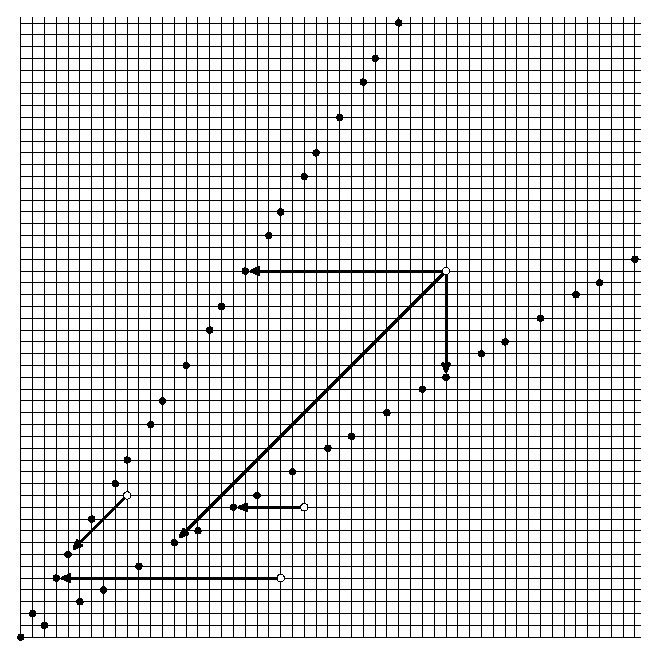
\includegraphics{mppics/pic-5}
\vskip-0mm
\caption{Проигрышные позиции и несколько выигрышных ходов.}
\label{pic:nim}
\end{figure}

Любая позиция с одной пустой кучей или с кучами одинакового размера автоматически выигрышная.
Не сложно понять, что самая простая проигрышная позиция это $\{1, 2\}$.
После этого можно увидеть, что $\{3, 5\}$, $\{4, 7\}$ и $\{6, 10\}$ также проигрышные.
Но где же закономерность?

Пусть $\{x_1 , y_1\}$, $\{x_2 , y_2\},\dots$ будут проигрышными позициями для первого игрока (не считая $\{0, 0\}$);
мы предполагаем что $x_i < y_i$ и $x_i < x_j$ при $i < j$.
Заметим, что $x_i \ne x_j$ для $i \ne j$, ведь если $x_i = x_j$, то Алекс мог бы сделать ход от большего из $y_i$ и $y_j$ к меньшему, оставляя Бет в проигрышной позиции --- противоречие.

Немного поразмыслив, приходим к выводу, что если известны все проигрышные позиции от $\{x_1 , y_1\}$ до $\{x_{n-1}, y_{n-1}\}$, то $x_n$ есть наименьшее положительное число, которого нет среди чисел из $\{x_1, \dots , x_{n-1}\} \z\cup \{y_1, \dots , y_{n-1}\}$, а $y_n = x_n + n$.
В этом случае $y_n$ больше любого числа из $\{x_1, \dots , x_{n-1}\} \cup \{y_1, \dots , y_{n-1}\}$.

Доказательство ведётся индукцией по $n$.
Мы уже знаем, что $x_n$ не может быть среди чисел в $\{x_1, \dots , x_{n-1}\} \cup \{y_1, \dots , y_{n-1}\}$, а также, что не может быть более одного $y_n$, который соответствует этому $x_n$.
Остаётся показать, что позиция $\{x_n, y_n\}$ проигрышная.

Если $\{x_n, y_n\}$ была бы выигрышной, то из неё можно было бы прийти в $\{x_i, y_i\}$ для некоторого $i < n$; но такой позиции нельзя достичь уменьшив меньшую кучу или уменьшив обе кучи на одинаковое число бобов, ведь это сделало бы разницу между двумя кучами $n$ или больше.
Также нельзя её достичь, уменьшив б\'{о}льшую кучу, ведь тогда был бы ещё один игрек для одного икса.
Таким образом, $\{x_n, y_n\}$ проигрышная.

Теперь можно получить список проигрышных позиций любой длины.
Из этого легко вывести стратегию Алекса.
Если он столкнётся с $\{x_i , y_i\}$, он убирает один или два боба и надеется на ошибку.
Если он видит $\{x_i , z\}$ для $z > y_i$, он уменьшает $z$ до $y_i$.
Если он видит $\{x_i , z\}$ с $x_i < z < y_i$, то есть разница $d = z - x_i < i$, он берет из обеих куч, чтобы дойти до $\{x_d , y_d\}$ (если $z = y_j$ для некоторого $j < i$, то у него также есть вариант уменьшить $x_i$ до $x_j$).
Если он видит $\{y_i , z\}$ с $y_i \le z$, то может уменьшить $z$ до $x_i$, а может иметь и другие варианты.


Однако, чтобы вычислить все проигрышные позиции, скажем до тысячи бобов в каждой куче потребуется значительное время.
Может можно найти более явное их описание?

Как мы уже знаем, $x_n$ лежит между $n$ и $2n$ для каждого $n$, ведь $x_n$ стоит сразу после всех $x_i$ и некоторых $y_i$ при $i < n$.
Разумно предположить, что $x_n$ примерно равно $rn$, для некоторого $r$ между $1$ и $2$.
Если это так, то $y_n$ примерно равно $rn + n = (r + 1)n$.

Если это подтвердится, то $n$ иксов между $1$ и $x_n$ примерно равномерно распределены, и, следовательно, доля $r/(r + 1)$ от их числа будет соответствующих игрекам ниже $x_n$.
Таким образом, у нас около $nr/(r + 1)$ игреков ниже $x_n$, и вместе с $n$ иксами, всего получается $x_n$ чисел; то есть
\[n+n\frac{r}{r+1}=nr,\]
что даёт нам $r + 1 = r^2$ или $r = (1 + \sqrt{5})/2$ --- знакомое \emph{золотое сечение}.

Наверное, теперь к вам на ум пришло блестящее наблюдение --- поскольку $r$ иррационально и $\tfrac1r+\tfrac1{r^2}=1$, числа $r$ и $r^2$($= r + 1$) подходят на роль $p$ и $q$ в решении «Надёжных мигалок» из главы 3.
Как мы знаем, любое положительное целое число представлено единственным способом как $\lfloor pm\rfloor$ для некоторого целого $m$, \emph{либо} как $\lfloor qn\rfloor$ для некоторого целого $n$.

А теперь уже возникает подозрение, что $x_n=\lfloor rn\rfloor$, а $y_n=\lfloor r^2 n\rfloor$.
Конечно же, эти значения обладают желаемыми свойствами:
каждое $x_n$ --- наименьшее положительное число, не из $x_1, \dots , x_{n-1}$ или $y_1, \dots, y_{n-1}$, иначе его было бы невозможно получить.
Остаётся проверить, что $\lfloor r^2 n\rfloor - \lfloor rn\rfloor = n$, но это легко, ведь $r^2 n - rn$ равно целому числу $n$,
поэтому и разница их целых частей обязана быть $n$ --- готово!

Забавы ради, давайте найдём ход Алекса из предложенных примеров.
Обратите внимание, что $12 000/r$ чуть меньше $7417$, и $7417r \z= 12 000{,}9581\dots$ так что $12 000$ это один из иксов, точнее $x_{7417}$.
Соответствующее значение $y_{7417}$ равно $\lfloor 7417r^2\rfloor = 19 417$, поэтому если в другой куче $20 000$ бобов, Алекс может выиграть, забрав из неё $20 000 \z- 19 417 = 583$ боба.
Если же в другой куче всего $19 000$ бобов, то Алекс может выиграть, уменьшив кучи одновременно до $\{x_{7000}, y_{7000}\} \z= \{11 326, 18 326\}$.

%\begin{addedbytheeditors}
%\textbf{Редакторам:} Добавил диаграмму.
%\end{addedbytheeditors}

\chapter{Новые встречи со старыми знакомыми}

\setlength{\epigraphwidth}{.53\textwidth}
\epigraph{Забыть ли дружбу прежних дней\\
И не грустить о ней?}{--- Роберт Бёрнс (1759---1796)}

Головоломки могут улучшаться с годами как вино, приобретая новые, захватывающие версии, а иногда и лучшие решения.
В этой главе представлены старые добрые многим знакомые головоломки.
Однако даже если вы очень хорошо знаете какие-то из них, 
вы обнаружите новые удивительные повороты!

Один из самых запоминающихся персонажей головоломок --- логик, любящий отдыхать на южных морях.
Если верить Мартину Гарднеру \cite{27}, он постоянно теряется и спрашивает дорогу у аборигенов.

\subsection*{Три аборигена на перекрёстке}\rindex{Три аборигена на перекрёстке}

Гарднеровский логик снова поехал на юг и, как обычно, стоит на развилке, желая узнать,  какая из двух дорог ведет в деревню.
На этот раз рядом с ним три аборигена, по одному из трёх племён:
племени правдолюбов,
племени лжецов
и племени случайно отвечающих.
Конечно же, логик не знает, к какому племени отнести каждого из аборигенов.
Ему разрешается задать только два вопроса с ответом «да» или «нет».
Каждый вопрос задаётся только одному аборигену.
Сможет ли он получить необходимую информацию?
А что если ему разрешено задать только \emph{один} вопрос с ответом «да» или «нет»?

\medskip

Перейдём к известной и изящной геометрической головоломке.
К моему стыду, она приведена с не вполне верным решением в моём предыдущем задачнике \cite{59}.

\subsection*{Новая встреча с тремя окружностями}\rindex{Новая встреча с тремя окружностями}

Назовём фокусом двух окружностей пересечение их общих внешних касательных.
Таким образом, если три окружности имеют разные радиусы (и ни одна не лежит в другой), то они определяют три фокуса (см. рис. \ref{pic:3circ}).
Докажите, что эти три фокуса лежат на одной прямой.

\begin{figure}[h!]
\centering
\includegraphics[scale=1]{pics/3circs}
\caption{Три окружности и их фокусы.}
\label{pic:3circ}
\end{figure}

\parit{Примечания.}
В моей предыдущей книге \cite{59} предлагалось построить три сферы с экваторами на данных окружностях, а затем рассмотреть плоскость, касающуюся этих трёх сфер.
Однако Джером Льюис, профессор информатики университета Южной Каролины в Апстейте, справедливо указал на то, что такой плоскости может и не быть!
Например, её нет, когда две окружности большие, а между ними находится меньшая.

Однако доказательство можно спасти, не отказываясь от основной идеи.
Попробуйте найти способ.

\medskip

Следующая задача --- отличный пример головоломок про знания о знаниях.

\subsection*{Самоубийцы Точкинска}\rindex{Самоубийцы Точкинска}

У каждого жителя Точкинска есть красная или синяя точка на лбу.
Если он когда-либо решит, что знает, какого цвета его точка, то покончит с собой.
Все точкинцы встречаются каждый день и видят друг друга.
Однажды приезжий сказал им что-то (что угодно не тривиальное) о числе синих точек.
Докажите, что рано или поздно все точкинцы покончат с собой.

\parit{Примечания.} Что-то \emph{нетривиальное} означает, что некоторое число синих точек делает это утверждение верным, а какое-то другое число --- неверным.
Однако мы не предполагаем, что приезжий сказал правду!
Увы, точкинцы легковерны --- они верят всему, что слышат, если только их собственные глаза не говорят обратное.

\medskip

Возможно, вы помните задачу об инфекции на шахматной доске --- прекрасную головоломку, в которой надо доказать, что нельзя заразить доску размера $n \times n$, начиная с менее чем $n$ заражённых клеток;
клетка заражается, если две или более из её соседей (по сторонам) заражены.
Доказательство, что $n$ заражённых клеток достаточно, было лёгкой частью; достаточно заразить клетки на главной диагонали.

А что если увеличить размерность?

\subsection*{Заражённые кубы}\rindex{Заражённые кубы}

Инфекция распространяется по $n^d$ единичным $d$-мерным кубам в кубе $n \times n \times \dots \times n$ следующим образом: если у единичного куба $d$ или более заражённых соседей, то он заражается.
(Соседями считаются кубы с общей гипергранью; в частности, у куба не может быть более $2d$ соседей.)

Докажите, что \emph{можно} заразить все кубы, начав с $n^{d-1}$ заражённых кубов.

\medskip

Задачи, где заключённые в красных или синих шляпах видят шляпы товарищей по несчастью и должны угадать цвет своей, произвели довольно много шума.
В версии, ставшей темой статьи в Нью-Йорк таймс \cite{50}, каждый заключённый мог выбрать, называть ему свой цвет или нет.
При этом все заключённые будут казнены, за исключением случая, когда все угадывающие правы и при этом нашёлся хотя бы один угадывающий.
Как обычно, заключённым было разрешено договориться заранее, но всякое общение прекращалось, как только они увидели шляпы.

Конечно же один заключённый может угадывать, а все остальные молчать --- 
это обеспечит 50\%-ю вероятность выживания. 
Может показаться, что лучшего добиться нельзя.
Однако есть гораздо лучшая стратегия --- $n$ заключённых смогут добиться того, чтобы вероятность казни была бы примерно $1/n$.

Для тех, кто считает такие задачи чересчур фантастичными, приготовьтесь:
скоро старые версии покажутся вам слишком реалистичными.

\subsection*{Шляпы и бесконечность}\rindex{Шляпы и бесконечность}\label{Шляпы и бесконечность}

На каждого из бесконечного множества заключённых, пронумерованных $1,2,\dots$, надета красная или синяя шляпа.
По сигналу все заключённые встают друг перед другом, так что каждый видит цвета всех шляп.
При этом никакое общение не позволяется.
Затем каждого заключённого отводят в сторону и спрашивают, какого цвета его шляпа.

Если ошиблось бесконечное число заключённых, то \emph{всех} казнят. 
У заключённых есть шанс сговориться заранее;
существует ли стратегия, которая обеспечит им выживание?

\parit{Примечания.}
Обратите внимание, что эта задача проще, чем описанная выше:
здесь нельзя молчать, нет никаких параметров и нет вероятности;
от вас требуется чистое решение.
Однако необходимо предположить, что каждый заключённый способен воспринять всю последовательность цветов шляп, которую он видит, и каким-то образом обработать всю эту информацию за конечное время, прежде чем высказать свою догадку.


\subsection*{Все правы или все неправы}\rindex{Все правы или все неправы}

На этот раз обстоятельства те же, но цель другая:
угадывания должны быть либо \emph{все верными}, либо \emph{все неверными}.
Существует ли выигрышная стратегия?

\parit{Примечания.}
Конечная версия этой задачи довольно лёгкая:
заключённые могут, например, заранее решить, что каждый будет угадывать цвет своей шляпы, предполагая, что общее число красных шляп чётно.
Если это на самом деле так, то все окажутся правы;
в противном случае все неправы.
Однако, если число красных шляп бесконечно, --- как определить, чётно ли оно?

\medskip

Вернёмся к конечному числу заключённых, но с числами вместо шляп.

\subsection*{Цифры на лбах}\rindex{Цифры на лбах}

На этот раз на лбу каждого из 10 заключённых написана цифра от 0 до 9 (например, все могут быть двойками).
В установленное время каждый будет поставлен перед всеми остальными, затем отведён в сторону, и его попросят угадать свою собственную цифру.

Для того чтобы избежать общей казни, хотя бы один из заключённых должен угадать правильно.
Как обычно, у заключённых есть возможность сговориться заранее.
Найдите для них стратегию, обеспечивающую выживание.

\subsection*{Заключённый дальтоник}\rindex{Заключённый дальтоник}

Заключённые из предыдущей головоломки вдруг узнают, что у одного из них (Шрека) зелёная кожа, а цифры будут написаны красным.
При этом другой заключённый (Майкл) страдает дальтонизмом, то есть не отличает красное от зелёного.
Поэтому Майклу придётся делать свои предположения только исходя из 8 видимых ему цифр.
Остальные заключённые, включая Шрека, по-прежнему смогут видеть все 9 цифр, кроме своей собственной.
Требуется доказать, что заключённые теперь уже не смогут гарантированно избежать казни.

\medskip

В последней из задач про заключённых числа встречаются со шляпами. 

\subsection*{Числа со шляпами}\rindex{Числа со шляпами}

На лбу каждого из $n$ заключённых написаны различные вещественные числа, так что каждый может видеть числа остальных, но не своё собственное.
Как обычно, после просмотра никакого общения не допускается, но затем каждый заключённый должен независимо выбрать себе шляпу --- либо красную, либо синюю.

Требуется, чтобы цвета шляп чередовались в порядке, определённом числами.

Игрокам разрешено сговариваться заранее.
Как им максимизировать вероятность успеха?

\medskip

Мы завершаем наши визиты к старым головоломкам одной задачей, которая берёт своё начало по крайней мере с середины девятнадцатого века, но не была решена до 2006 года.
Мы не будем просить вас доказывать правильность вашего решения (хотя, конечно, вы можете попробовать) --- для разгадки этой головоломки потребовались пять профессиональных математиков, и даже сейчас ответ известен только с точностью до постоянного множителя.
Однако угадывание конструкции --- отличная проверка вашей интуиции.

\subsection*{Кирпичная стенка}\rindex{Кирпичная стенка}\label{Кирпичная стенка}

На какое максимальное расстояние стенка из $n$ кирпичей может зайти за край стола?

\parit{Примечания.} Предполагается, что кирпичи --- однородные прямоугольные твёрдые тела длины 1 без трения;
их ставят горизонтально в общей вертикальной плоскости.
Однако не нужно предполагать, что на каждом уровне находится только один кирпич.

\section*{Источники и решения}

\subsection*{Трое аборигенов на перекрёстке}

Этот вариант зачачи про логика и аборигенов пришёл ко мне от двух матфизиков, Владаса Сидоравичюса и Сени Шлосмана.
Кажется, что случайный абориген путает все карты, однако задачу решить можно.

Сначала надо позаботиться о том, чтобы второй спрошенный абориген не был из случайного племени.
Это необходимо, так как за один вопрос дорогу не узнать, и при этом если второй абориген случайный, то вы не узнаете ничего больше.

С другой стороны, этого должно хватить, ведь далее можно использовать традиционный вопрос типа «А если бы я спросил вас, ведет ли первая дорога к деревне, вы бы сказали „да“?»

Чтобы достичь этой цели, вам нужно будет задать аборигену А что-то об оборигенах Б или В, а затем использовать ответ, чтобы выбрать между Б и В.
Вот вариант, который работает: «Верно ли, что Б ответит правду, с большей вероятностью чем В?»

Забавно, что если А ответит «да», то надо выбирать В, а если «нет», то выбираете Б!
Ведь если А говорит правду, вы хотите обратиться к тому, кто меньше всего склонен говорить правду, то есть к лжецу.
Если же А лгун, то вам нужен более правдивый из его спутников, а именно правдолюб.

Конечно же, если А --- случайный, то нет значения, к кого выбрать из Б и В вы обратитесь.

В колонках Мартина Гарднера отмечалось, что в первоначальной задаче с одним аборигеном логик может дойти до деревни даже если он забыл, что означает слово каждого на местном языке (предполжительно «да» и «нет»).
Читатели, желающие поразвлечься, могут попытаться аналогично изменить вышеуказанный протокол.

Если случайный абориген решает сказать «да» или «нет», подбрасывая монету в уме, то, конечно же, одного вопроса недостаточно.
Однако, если предположить, что он случайно выбирает между правдой и ложью, а затем отвечает логически,
то для этого случая Анупам Джайн из Университета Южной Калифорнии придумал следующий вопрос:

\begin{itemize}
 \item[] \emph{Если я выберу из двух ваших спутников того, чей ответ с наименьшей вероятностью будет совпадать с вашим, и спрошу его, ведёт ли первая дорога в деревню, он ответит ли он „да“?}
\end{itemize}

Утверждается, что если ответ «нет», то первая дорога --- правильная, в противном случае вторая.

Критический случай возникает, когда логик задает этот вопрос случайному отвечающему. Если случайный отвечающий решил солгать на этот вопрос, то ответ искреннего парня на вопрос будет наименее вероятно соответствовать его искренности. Искренний парень скажет «да», и так как случайный отвечающий решил солгать, он скажет противоположное и, таким образом, ответит «нет». Если случайный отвечающий решил сказать правду на этот вопрос, то искреннего парня ответ будет наименее вероятно соответствовать его искренности. Лжец скажет «нет», и так как случайный отвечающий решил сказать правду, он также скажет «нет».

Если логик обращается к человеку, говорящему правду, то это будет лжец, чья искренность наименее вероятно совпадет с его искренностью, и он скажет то, что сказал бы лжец: «нет».

Точно так же, если Дорога 2 - правильная дорога, все ответы будут «да».

\chapter{Серьёзные испытания}


\setlength{\epigraphwidth}{.80\textwidth}
\epigraph{Со временем разум достигнет более высокого уровня знаний, но не сможет понять, как он там оказался.
%There comes a time when the mind takes a higher plane of knowledge but can never prove how it got there.
}{--- Альберт Эйнштейн (1879---1955)}

Ну да, как будто предыдущие головоломки не были сложными, а тут ещё несколько непростых задач.
Хотя может случиться, что некоторые из них покажутся проще.
Ведь то, что ставит одного в тупик, бывает легко другому.


\subsection*{Торт-мороженое}\rindex{Торт-мороженое}\label{Торт-мороженое}

Перед нами цилиндрический торт-мороженое покрытый сверху шоколадной глазурью.
Мы последовательно отрезаем от него дольки с углом $x$, где $x$ произвольно,
каждый раз долька переворачивается и вставляется обратно в торт
(рис. \ref{pic:tort}).

Докажите, что после конечного числа таких операций вся глазурь снова окажется сверху!


\begin{figure}[htb!]
\centering
\includegraphics[scale=1]{pics/tort}
\caption{Разрез, переворот, и снова разрез.}
\label{pic:tort}
\end{figure}

\parit{Примечание.}
Я называю такие задачи \emph{как бы неверно услышанные}.
Да-да, угол $x$ может быть иррациональным. 
В этом случае вы никогда не отрежете одинаковый кусок дважды.
Придётся отрезать довольно много долек, но всё же хватит конечного числа.
К счастью, торт-мороженое самовосстанавливается.

\subsection*{Прыгание и перепрыгивание}\rindex{Прыгание и перепрыгивание}

Лягушка прыгает по длинной цепочке кувшинок;
на каждой кувшинке она подбрасывает монету, чтобы решить,
сделать ли ей двойной прыжок вперёд или же одинарный назад.
На какой доле кувшинок она побывает?

\subsection*{Три тени кривой}\rindex{Три тени кривой}\label{Три тени кривой}

Существует ли простая замкнутая кривая в трёхмерном пространстве, все три проекции которой на координатные плоскости являются деревьями?

\parit{Примечание.}
Это означает, что тени кривой в трёх координатных направлениях не содержат циклов.
На рис. \ref{pic:proj1} изображена кривая, которая почти подходит: две её тени являются деревьями, но третья содержит (и даже является) циклом.

\begin{figure}[htb!]
\centering
\includegraphics[scale=1]{pics/proj1}
\caption{Кривая у которой две проекции --- деревья, а третья --- нет.}
\label{pic:proj1}
\end{figure}

\subsection*{Игроки и победители}\rindex{Игроки и победители}

Тристану и Изольде предстоит очутиться в ситуации с очень ограниченной связью, в которой Тристан будет знать, какие две из 16 баскетбольных команд сыграли матч, а Изольда узнает, кто выиграл.
Сколько битов необходимо передать им друг другу, чтобы Тристан узнал, кто одержал победу?


{\sloppy

\parit{Примечание.}
Эта задача по \emph{коммуникационной сложности}.
Если Изольда знает, кто играл и кто выиграл, то ей достаточно отправить Тристану один бит, сообщив, скажем, выиграла ли команда, идущая первой по алфавиту.
Без этой информации она могла бы просто отправить четыре бита, чтобы определить победившую команду.
А можно ли обойтись меньшим числом битов?

}

\medskip

А вот ещё задача по коммуникационной сложности, но посложней.

\subsection*{Подсказка для Чарли}\rindex{Подсказка для Чарли}

Алиса и Боб знают да-нет ответы на все $n$ вопросов экзамена, который сдаёт Чарли.
Чарли нужен только ответ на $k$-й вопрос, но ни Алиса, ни Боб не знают значение $k$.
Вместо этого Алиса знает число $i$, Боб --- число $j$, такие, что $k = i + j \pmod n$.
При этом Чарли знает оба числа $i$ и $j$.

Если бы Алиса не могла передать никакой информации,
то Бобу пришлось бы отправить Чарли все ответы (всего $n$ битов), чтобы Чарли смог узнать нужный ему ответ.

Докажите, что если Чарли получит всего один бит от Алисы, то Бобу достаточно отправить всего $n/2$ битов.

\subsection*{Сближение по кривой}\rindex{Сближение по кривой}

\begin{figure}[htb!]
\centering
\includegraphics[scale=1]{pics/s-curve}
\caption{Кривая с обоими свойствами.}
\label{pic:s-curv}
\end{figure}

Плоская кривая на рис. \ref{pic:s-curv} обладает следующими свойствами:
(1) расстояние между её конечными точками больше, чем у любой другой пары точек на кривой (мы используем обычное евклидово расстояние на плоскости),
и
(2) взяв по карандашу в обе руки, можно поставить их кончики в концах кривой и двигать их вдоль кривой до встречи, так, чтобы \emph{в процессе расстояние между ними не увеличивалось}.

Существует ли кривая со свойством (1), но без свойства (2)?


\subsection*{Суммы и произведения}\rindex{Суммы и произведения}

В шляпе лежат все целые числа, большие 1, но меньшие 100.
Из неё достают два числа.
Саманта узнаёт их сумму, а Порфирио --- их произведение.
Далее, Саманта говорит:

--- Я знаю, что ты не знаешь этих чисел.

--- Теперь я их знаю, --- отвечает Порфирио.

--- Теперь и я знаю, --- говорит Саманта.

Что это были за числа?

\begin{figure}[htb!]
\centering
\includegraphics[scale=.95]{pics/korona}
\caption{Корона.}
\label{pic:korona}
\end{figure}

\begin{figure}[htb!]
\centering
\includegraphics[scale=.95]{pics/wreath}
\caption{Венок.}
\label{pic:wreath}
\end{figure}

\begin{figure}[htb!]
\centering
\includegraphics[scale=.95]{pics/treug}
\caption{Схлопнутый треугольник.}
\label{pic:treug}
\end{figure}

\subsection*{Складной многоугольник}\rindex{Сложенный многоугольник}\label{Сложенный многоугольник}

Какова минимальная площадь простого нечётноугольника, с единичными сторонами?

\parit{Примечание.}
Простой многоугольник это замкнутая ломаная без самопересечений, состоящая из конечного числа звеньев.
Многоугольник не обязан быть выпуклым,
например, он может выглядеть как один из многоугольников на рис. \ref{pic:korona},
\ref{pic:wreath} и \ref{pic:treug}.
Очевидно, что у многоугольника на рисунке \ref{pic:treug} площадь не менее площади равностороннего треугольника с единичными сторонами, то есть $\sqrt{3}/4$.
Несложно проверить, что и площадь короны на рис. \ref{pic:korona} ограничена тем же числом.
Но про венок на рис. \ref{pic:wreath} это уже не так очевидно.

Равносторонние \emph{чётно}угольники могут иметь произвольно малую площадь, например, складываясь в очень остроконечную звезду.
А что по поводу нечётноугольников --- могут ли они иметь площадь меньше $\sqrt{3}/4$?
Сможете ли вы это доказать или опровергнуть?


\section*{Источники и решения}

\subsubsection*{Торт-мороженое}

Эта замечательная головоломка досталась мне от французского аспиранта Тьерри Мора,
а тот узнал её от своего школьного учителя Томаса Лаффорга.
Головоломка (происхождения которой Лаффорг точно не знает) на самом деле включала в себя ещё один угол, определяющий зазор между дольками торта.
Даже в этом случае, глазурь ухитрится вернуться наверх после конечного числа операций;
упорные читатели могут в этом убедиться.
Наша формулировка (с нулевым зазором) уже достаточно удивительна и, думается, что достаточно сложна.

Если вы решили, что при иррациональном $x$ понадобится бесконечное число операций, то вы совсем не одиноки.
В конце концов, если $n$ операций достаточно, то $n$-ый разрез, должен пройти по границе области покрытой глазурью;
как же смогла эта линия оказаться там, где торт никогда не разрезался?

Однако она там окажется, причина в том, что когда долька переворачивается, её покрытая и непокрытая области  меняются не только местами, но и порядком.

В этой головоломке, как и во многих алгоритмических задачах, полезно переопределить операцию так, чтобы менялось только состояние (в данном случае, область покрытая глазурью), а не сама операция, которая пока что у нас меняется на каждом шагу.
В нашем случае достаточно добавить поворот торта после каждой операции так, чтобы разрез всегда приходился на одно и то же место.


\begin{figure}[htb!]
\centering
\includegraphics[scale=.9]{pics/tort2}
\caption{Разрезы и перевороты с вращением.}
\label{pic:tort2}
\end{figure}

Будем считать, что $0\degree$ --- направление на север,
$90\degree$ --- на восток и так далее.
Каждый раз будем разрезать по направлениям $0\degree$ и $-x$.
Затем кусок переворачивается через линию $0\degree$ и оказывается между $0\degree$ и $x$.
В это же время остальная часть торта поворачивается по часовой стрелке на угол~$x$.
На рис. \ref{pic:tort2} пунктирные линии показывают где проходят разрезы на первых четырёх шагах.

Чтобы понять дальнейшее рассуждение, проще всего думать, что $x$ чуть больше $360\degree/k$ для некоторого целого $k$.
В этом случае первый разрез по дольке произойдёт на $k$-м шаге, после того как торт развернётся на полный оборот.

Пусть $k$ --- наименьшее число долек, которое надо вырезать, чтобы добраться до конца торта.
Другими словами, $k$ --- наименьшее целое число, большее или равное $360\degree/x$.
Тогда $x \z= y + z$, где $y = 360\degree/k$ и 
\[0\le z <\frac{360\degree}{k-1}-\frac{360\degree}{k}=\frac{360\degree}{(k-1)k}.\]
Конечно же, если $z = 0$, то $x = y = 360\degree/k$, и тогда $k$ операций переведут всю глазурь на дно торта, а ещё $k$ вернут её наверх.
В противном случае, как мы увидим, невозможно достичь момента, когда вся глазурь окажется снизу.

По мере выполнения шагов, будут появляться граничные линии (между покрытой и непокрытой областями) под углами $0$, $x$, $2x$, $3x, \z\dots , (k - 1)x$, а затем $x - kz$, $2x - kz$, $3x - kz, \dots , (k - 1)x - kz$,
и затем они повторяются.
Действительно, легко проверить, что описанный набор $S$ граничных линий замкнут относительно операции разрез-переворот-поворот.
Одна такая операция переносит $ix$ в $(i + 1)x$, кроме $(k - 1)x$, который переносится в $x - kz$;
она же переносит $ix - kz$ в $(i + 1)x - kz$, кроме $(k - 1)x - kz$, который идёт в $x$.
Тем временем разрез $0\degree$ всё время остаётся на месте.
Отсюда следует, что набор граничных линий всегда является подмножеством $S$.

Уже можно заключить, что конечное число операций вернёт всю глазурь на верх, ведь у нас только $2k - 1$ областей торта между $2k - 1$ линиями из $S$.
Каждая область может быть покрыта или не покрыта глазурью, поэтому число достижимых конфигураций не превышает $2^{2k-1}$.
Значит процесс зациклится за не позже чем за $2^{2k-1}$ шагов.
Но обязательно ли мы вернёмся к начальной конфигурации (все области покрыты глазурью)?
Да, потому что операция обратима.
Если бы процесс зациклился на другой конфигурации $C$, то существовали бы две разные конфигурации, которые приводили бы к $C$, а это невозможно.

Однако несложно понять в точности, что и как происходит.
Между граничными линиями в $S$ есть $k$ областей с углом $x - kz$ --- назовём их $A_1$, $A_2, \dots , A_k$, и ещё $k - 1$ область с углом $kz$ --- назовём их $B_1$, $B_2, \dots , B_{k-1}$.
(На рис. \ref{pic:tort3} показан случай $k = 4$ при $x = 93{,}5\degree$.)

\begin{figure}[htb!]
\centering
\includegraphics[scale=1]{pics/tort3}
\caption{Области при $x = 93{,}5\degree$ и значит $z = 3{,}5\degree$.}
\label{pic:tort3}
\end{figure}

С начала процесса, $A$-области становятся не покрытыми глазурью, по порядку.
После $k$ операций все они становятся не покрытыми.
Затем они снова покрываются глазурью, снова по порядку, до тех пор, пока после $2k$ операций все покроются глазурью.
Тем временем $B$-области также становятся не покрытыми глазурью по порядку.
Поскольку их только $k - 1$, после $k - 1$ шагов все они станут не покрытыми, и все снова покроются после $2k - 2$ шагов.

Значит число шагов, необходимых чтобы покрыть глазурью оба типа областей, является наименьшим общим кратным $2k$ и $2k \z- 2$, то есть $2k(k - 1)$.
Значит потребуется $2k(k - 1)$ шагов, конечно если $x \z\ne 360\degree/k$ для некоторого целого $k$ ---
в этом случае $B$-области отсутствуют и достаточно $2k$ шагов.

Рассуждая таким же образом, заключаем, что если все области не покрыты глазурью после $n$ шагов,
то $n$ должно равняться нечётному числу домноженному на $k$
и в то же время нечётному числу домноженному на $k - 1$.
Поскольку ровно одно из чисел $k$ и $k - 1$ нечётно, $n$ чётно и нечётно одновременно,
что невозможно.
Значит, если есть $B$-области, то вся глазурь никогда не окажется снизу.

А вот реакция на эту головоломку одного очень известного математика:
«Трудно поверить, что вся глазурь вернётся наверх.
Но если уж это произойдёт, то я уверен, что в какой-то момент, вся глазурь окажется снизу!»

\begin{addedbytheeditors}
\textbf{Редакторам:} На картинке $x4z\to x-4z$
\end{addedbytheeditors}

\subsubsection*{Прыгание и перепрыгивание}

Эту на вид простую головоломку придумал Джеймс Б. Ширер --- математик из IBM,
она появилась на сайте головоломок IBM \cite[апрель 2007]{ponder-this}.
Головоломка вовсе не такая простая, но она колется парой полезных трюков.

Пронумеруем кувшинки по порядку.
Естественно начать с подсчёта вероятности $p$ того, что лягушка, стартуя с $1$, вернётся в какой-то момент в $0$.
Чтобы никогда не возвращаться, она должна совершить прыжок вперёд (вероятность $1/2$) и не вернуться обратно трижды (вероятность $1 - p^3$).
Таким образом, $(1 - p) = \tfrac12(1 - p^3)$.
Поделив на $(1 - p)/2$, получим, что $2 = 1 + p + p^2$, а это даёт $p = (\sqrt5 - 1)/2 \z\sim 0{,}618034$ --- знакомое золотое сечение.

Однако подсчитать вероятность того, что лягушка перескакивает конкретную позицию (скажем, $1$) так легко не получается.
Можно было бы начать вычисления с момента, когда лягушка первый раз попадает в $0$, ведь если это не произошло, то ей придётся попасть в~$1$.
Однако легче вычислить вероятность того, что во время конкретного прыжка лягушка перескакивает через кувшинку, которую она  не посещала и не посетит.

Для того чтобы это произошло, лягушка должна
(а) прыгать вперёд в данный момент,
(б) никогда не возвращаться обратно от того места, где она приземлилась,
и (в) не посещала ту кувшинку, через которую она прыгает, в прошлом.

Мы можем считать, что кувшинка, которую перепрыгивает лягушка, имеет номер 0.
Ключ в том, что если развернуть нумерацию и время, то событие (в) становится независимой копией события (б).
Иначе говоря, лягушка ведёт себя ровно также если обратить время и рассматривать кувшинки в обратном порядке ---
она равновероятно прыгает на два вперёд или на один назад.
Событие (в) означает, что достигнув $-1$, она не «вернётся» в $0$.

Таким образом, вероятность того, что все три события произойдут, составляет $1/2 \cdot (1 - p) \cdot (1 - p) = (1 - p)^2 / 2$.
Однако это ещё не вероятность того, что $0$ пропускается, а только вероятность того, что в данный момент лягушка перепрыгивает через пропущенную кувшинку.

Поскольку лягушка, в среднем, перемещается со скоростью $1/2$, она производит $(1 - p)^2$ пропущенных кувшинок на единицу пройденного пути.
Отсюда следует, что доля кувшинок, на которые она попадает, составляет $1 - (1 - p)^2 \z= (3\sqrt5 - 5) / 2 \sim 0{,}854102$.

\subsubsection*{Три тени кривой}

Эту головоломку мне подбросил Рик Кенион (Университет Британской Колумбии), который увидел её на двери Джорджа Бергмана в Бёркли. 
Бергман услышал её от Хендрика Ленстры из Бёркли и Университета Лейдена.
По словам Бергмана, Ленстра видел игрушку, состоящую из кубической пластиковой коробки с прорезями, образующими своего рода лабиринт на каждой грани, при этом каждая пара противоположных граней имела одинаковые прорези, так что стержень, перпендикулярный этим двум граням, мог бы одновременно проходить через два лабиринта.
Но вместо одного стержня был объект, который, по сути, состоял из трёх взаимно перпендикулярных стержней, соединённых в точке, при этом каждый стержень проходил через лабиринты на паре противоположных граней коробки.
Цель игры заключалась в том, чтобы добраться из одной позиции в другую.

\begin{figure}[t!]
\centering
\includegraphics[scale=1]{pics/tree3}
\caption{Кривая три тени которой деревья.}
\label{pic:tree3}
\end{figure}

Кстати, эту головоломку теперь можно купить.
%ссылка не работает??? http://bitsandpieces.com/ˆBrainteasersˆMetal+Puzzles/07-W7871.html. 
Её придумал Оскар ван Девентер --- блестящий голландский изобретатель, чьи механические головоломки часто воплощают увлекательные математические идеи.

Так или иначе, Ленстра обратил внимание на то, что лабиринт на каждой грани обязан быть деревом,
если бы он имел замкнутый цикл, то часть пластика вывалилась бы.
Тогда он задался вопросом, какова будет область доступных позиций для центральной точки трёх стержней.
Её проекция на каждую грань должна быть деревом, но может ли это множество само иметь цикл?
Если да, то такой цикл должен был проецироваться на каждую грань как дерево.
Так и возник вопрос.

Ленстра задумался над этим в феврале 1994 года, или около того.
Бергман расспрашивал об этом разных людей, но безуспешно.
Наконец, в сентябре 1995 года Кевин Буззард, в то время постдок в Бёркли, сообщил Бергману и Ленстре, что вопрос был известен ещё раньше в Кембридже (Англия), и нашёлся пример.
Буззарду этот пример показал Имре Лидер, комбинаторик из Кембриджского университета, который услышал о нём от Джона Рикарда, который его и придумал.
Рикард работал на математичеком отделении Кембриджа, но теперь программист.

Пример Рикарда, который обладает очень красивой шестикратной симметрией, изображён на рис. \ref{pic:tree3}.

\subsubsection*{Игроки и победители}

Эта задача ко мне пришла от Алона Орлицкого из Университета Калифорнии в Сан-Диего.
Она иллюстрирует силу коммуникации \emph{от студента к учителю}.

Тристан и Изольда могут заранее пометить команды четырёхзначными двоичными числами от 0000 до 1111 в алфавитном порядке. Затем, когда Тристан узнает, кто играл, он может отправить Изольде 00, 01, 10 или 11 передав \emph{первую позицию в которой отличаются две метки команды}, это может быть первый, второй, третий или четвёртый бит.
Изольде следует отправить обратно значение этого бита.

Например, если команда 0110 играла с командой 0011, и одержала победу,
то Тристан отправит Изольде «01», указывая, что метки играющих команд, отличаются во втором бите.
Изольда отправит обратно «1» --- значение второго бита победившей команды.

Эта схема требует отправки трёх битов, на один меньше, чем метод, при котором Изольда просто отправляет метку победившей команды.
Однако на самом деле этот бит даёт экспоненциальное улучшение!
Если у нас $n = 2^{2^k}$ команд, то один метод требует $2^k$ битов, а другой всего $k + 1$.


\begin{addedbytheeditors}
 \textbf{Редакторам:} Возможно «от студента к учителю» надо переводить иначе.
Кто-нибудь владеет терминологией сложности коммуникаций?
 \end{addedbytheeditors}

\subsubsection*{Подсказка для Чарли}

На самом деле это серьёзная задача по сложности коммуникаций.
Она была рассмотрена Лесом Валиантом из Гарварда в 70-х годах,
а сообщил мне о ней Амит Чакрабарти из Дартмутского колледжа.
Решения этой и более общей задачи приведены в статье Павла Пудлака, Войтеха Рёдля и Йижи Шгалла \cite{49}.

Пусть $x_1, \dots , x_n$ --- биты, представляющие ответы, где (допустим) $1 = \text{«да»}$ и $0 = \text{«нет»}$.
Индексы берутся по модулю $n$.
Алиса отправляет Чарли $x_{-i}$,
а Боб отправляет Чарли все значения $x_a + x_b$ для всех пар $(a, b)$, таких что $a + b = j$;
сумма битов берётся по модулю $2$.
Обратите внимание, что таких пар $n/2$ (после округления вверх, если $n$ нечётное).

Чарли знает $x_{-i}$, а также $x_{-i} + x_{i+j}$, сложив их, он получит $x_{i+j}$.

Выглядит просто, но догадаться сложно.

\begin{addedbytheeditors}
\textbf{Редакторам:} Вроде ответ $\lfloor n/2\rfloor$, но этого НЕ сказано.
Думаю надо добавить в скобки «; однако в этом случае, есть пара $(a,b)$, такая, что $a=b$ и её можно пропустить.»)
\end{addedbytheeditors}

\subsubsection*{Сближение по кривой}

Этим вопросом меня озадачил Оскар ван Девентер, тот, что уже упоминался выше.
Он думал использовать такую кривую в механической головоломке.
Такие кривые на самом деле существуют, сложнее найти пример для которого можно доказать, что он не обладает вторым свойством.

На рис. \ref{pic:ss-curve} показана такая кривая, которую по своим причинам ван Девентер называет \emph{неконкинкульной}.
%non-conquinculous

\begin{figure}[htb!]
\centering
\includegraphics[scale=1]{pics/ss-curve}
\caption{Кривая со свойством (1), но без сойства (2).}
\label{pic:ss-curve}
\end{figure}

Пунктирный круг на рисунке добавлен для того, чтобы сразу стало ясно то, что кривая удовлетворяет первому свойству.
Остаётся убедиться, что для неё второе свойство не выполнено.
Предположим обратное, и пусть $t$ --- первый момент времени, когда один карандаш пройдёт от белого квадрата до белой стрелки,
либо же другой пройдёт от серого квадрата, до серой стрелки.
Какое-то время \emph{до} момента $t$ два карандаша должны оказаться друг напротив друга, как белый и серый круги.
Но \emph{после} времени $t$ им придётся разойтись, чтобы сойтись вместе, и это приведёт к увеличению расстояния.

Но как найти такую кривую?
(Если вопрос пугает, то пропустите следующие три абзаца.)
Представьте себе, что кривая параметризована параметром $t$;
это означает, что существует непрерывная функция $C$ из $[0, 1]$ в плоскость такая, что $C(0)$ --- один конец кривой (скажем, левый), $C(1)$ --- другой её конец, и $C(t)$ описывает кривую когда $t$ идёт $0$ до $1$.
Успешное управление карандашами в соответствии со свойством (2) означает пару непрерывных функций $f$ и $g$ из $[0,1]$ в себя, где в момент времени $t$ карандаши расположены в точках $C(f(t))$ и $C(g(t))$.
Таким образом, $f (0) = 0$, $g(0) = 1$, $f (1) = g(1)$, и расстояние от $C(f (t))$ до $C(g(t))$ не убывает при увеличении $t$.
Вместе $f$ и $g$ описывают кривую от $(0,1)$ до линии $x = y$, в треугольнике с вершинами в $(0,1)$, $(0,0)$ и $(1,1)$.

Для того чтобы это стало невозможно, хотелось бы иметь \emph{двойственный путь} между прямыми $x = 0$ и $y = 1$, не заходящий на $x = y$, и соотвтестующий парам точек на локально минимальном расстоянии.
Если такая кривая нашлась, то она пересекается с нашей кривой $(f, g)$, а это влечёт подъём расстояния.

Этот двойственный путь соответсвует другому виду манипуляций с карандашами:
начинём с левого карандаша в левой конечной точке и правого карандаша где-то на кривой,
затем перемещаем обе точки в одном направлении вдоль кривой, пока правый карандаш не достигнет правой конечной точки.
Если при этом ни одну точку нельзя переместить относительно другой без увеличения расстояния между ними, то мы достигли цели.
На данной фигуре карандаши начинают с белого квадрата и серой стрелки, затем движутся вместе, пока не достигнут белой стрелки и серого квадрата, соответственно.

\medskip

В награду за этот пример ваш автор получил прототип механической головоломки, замечательной как и все творения ван Девентера.

\subsubsection*{Суммы и произведения}

Эта забавная головоломка всплывала на различных формах в течение многих лет; она появилась в колонке Мартина Гарднера для Scientific American в декабре 1979 года, но по какой-то причине не вошла в сборник задач этой колонки \cite{29}.
Кажется удивительным, что столь туманной информации может хватить.

Головоломка, по сути та же, что наша, была предложена независимо Стивом Феннером из Университета Южной Каролины и Биллом Готтесманом, разработчиком и производителем солнечных часов.
Ход рассуждений ниже предложен Готтесманом.

Для начала, обозначим число Порфирио через $P$, а число Саманты через $S$, и пусть $\{X, Y\}$
--- неизвестная пара.
Вначале Порфирио не знает ответа, значит числа $X$ и $Y$ не могут быть оба простыми,
ни простым и его квадратом,
ни простым и его кубом.
Более того, ни одно из них не может быть большим простым числом (больше чем $50$), так как в этом случае оно должно было бы быть одним из сомножителей~$P$.

Следовательно, поскольку Саманта заранее знает, что Порфирио не может знать ответ,
$S$ не может быть больше $53$ или же равно сумме двух простых чисел.
Это исключает все чётные числа --- гипотеза Гольдбаха, проверенная далеко за $53$, гласит, что каждое чётное число больше $2$ является суммой двух простых.
Остаются только некоторые из чисел, превышающие какое-то нечётное составное число на $2$, а именно
$11$, $17$, $23$, $27$, $29$, $35$, $37$, $41$, $47$ и $53$.
(Например, $51=34+17$ и число $34\times 17$ допускает единственное разложение на сомножители до $100$.
Поэтому $51$ не золотое, хотя и превышает на $2$ составное число $49$.)
Готтесман назвал эти числа \emph{золотыми}.
Не нужно беспокоиться о суммах простого числа и его квадрата или куба, так как они все чётные.

Из того, что Порфирио теперь уже знает $X$ и $Y$ (и из того, что сумма и произведение двух положительных целых чисел полностью их определяет), можно вывести, что множители всего одного раложения $P$ дают золотую сумму. 
Каждое золотое число $G$ даёт Саманте $(G - 3)/2$ возможных пар $\{X, Y\}$
(например, для $11$ можно собрать как $2 + 9$, $3 + 8$, $4 + 7$ или $5 + 6$); должно оказаться, что только одна из этих пар имеет произведение $P$ с желаемым свойством.
Если $G = 11$, то первые две пары выше уже позволяют Порфирию вывести $X$ и $Y$.
Для случая $2 + 9$, получаем $P = 18$, и оно раскладывается только как $2 \times 9$ (где $2 + 9 = 11$ является золотым) или как $3 \times 6$ (дающее на золотую сумму $S = 13$).
В случае $3 + 8$, получаем $P = 24$, оно раскладывается как $2 \times 12$ (а $14=2+12$ не золотое) или
$3 \times 8$ (и $11=3+8$ золотое) или $4 \times 6$ (а $10=4+6$ не золотое).
Таким образом, $G$ не может быть $11$.

Следующее золотое число, $17$, подходит!
Ровно одна пара слагаемых даёт $P$, у которого единственная золотая сумма множителей равна $17$, а именно $4$ и $13$ (поскольку $2 + 26 = 28$, не золотое).

Надо ещё перебрать остальные шесть пар слагаемых для $17$, чтобы убедиться, что ни одна из них не даёт подходящего $P$.
Это даёт надежду, что $X$ и $Y$ могут быть $4$ и $13$.
Остаётся проверить, что $\{4, 13\}$ --- единственный ответ.
Для этого придётся повторить весь процесс для остальных восьми золотых чисел, 
и мы убедимся, что ни одно из них не подходит.

Решение этой головоломки не достаточно изящно,
хоть я и объявил красоту необходимым требованием (для решённых головоломок).
Однако то, что услышав этот короткий разговор, можно восстановить числа не зная ни суммы ни произведения, должно служить небольшим вознаграждением.

\begin{addedbytheeditors}
\textbf{Редакторам:}
Я не понял зачем говорить о квадратах и кубах.
И не понял почему не золотые 23 и 29.
(И нет охоты понимать.)
Почему там стоит 53 --- 53 это первое простое после 50, а числа начинаются с 2 --- вроде должно быть 54?
(Последнее конечно не влияет на рассуждение.) 
\end{addedbytheeditors}

\subsubsection*{Сложенный многоугольник}

Эта головоломка пришла ко мне (как открытый вопрос) от Роберта Вейта из Юго-Восточного университета Индианы, который долго и тщетно пытался её решить.
Мне удалось найти (на мой взгляд) изящное решение, представленное ниже.
Позже выяснилось, что задачу уже решили К. Бёроцки, Г. Кертеша и Э. Макая \cite{9}.

Ответ такой: У каждого нечётноугольника с единчными сторонами площадь не меньше $\sqrt{3}/4$, причём равенство достигается только для треугольника.

Как такое можно доказать?
Утверждение тривиально для треугольников,
и естественно возникает искушение воспользоваться индукцией по числу сторон.
Как мы увидим,  многоугольник с четырьмя и более сторонами можно разрезать диагональю на два многоугольника с меньшим числом сторон у каждого.
Однако, вообще говоря, новые многоугольники не будут равносторонними.
Таким образом, нужно придумать индукционное предположение применимое к более широкому классу многоугольников, возможно, ко \emph{всем}.

Приведённое ниже индукционное предположение отлично работает, хоть и выглядит топорно.
Важно правильно подобрать параметр.

Обозначим через $\mathbb{O}^n$ множество всех целочисленных $n$-векторов нечётного веса, то есть 
\[\mathbb{O}^n=\left\{\,\vec x=(x_1,\dots,x_n)\in \mathbb{Z}^n\,\middle|\, \sum_ix_i\equiv 1\pmod 2\,\right\}.\]
Чтобы измерить насколько многоугольник $P$ близок к нечётноугольнику с единичными сторонами, мы воспользуемся параметром $u(P)$, назовём его \emph{несложимостью} $P$, определённым как
\[u(P)=1-\min_{\vec x\in \mathbb{O}^n} \left\{\sum_i |e_i-x_i|\right\}.\]
где  $e_1,\dots,e_n$ --- длины сторон $P$.
Заметим, что $u(P)\z\leqslant1$, и $u(P)\z=1$ если $P$ --- нечётноугольник с единичными сторонами, или даже любой многоугольник с целочисленными сторонами и нечётным периметром.
С другой стороны, $u(P)\leqslant 0$ если, например, две из сторон многоугольника $P$ имеют длину $\tfrac12$, или же если его периметр является чётным целым числом.

Многоугольник будет считаться \emph{хорошим}, если у него нет вырожденных вершин,
то есть нет вершин с внутренним углом $180\degree$.
Если $P$ имеет стороны длины больше~$1$, то из него можно получить (возможно нехороший) многоугольник $P^*$ со сторонами длины не более~$1$, подразбив каждую длинную сторону $P$.
При этом, можно добиться что бы $u(P^*)=u(P)$.

Теперь мы переходим к индукционному доказательству того, что площадь $A(P)$ любого многоугольника $P$ не меньше $\tfrac{\sqrt{3}}{4}u(P)$.
Отсюда немедленно последует, что площадь нечётноугольника с единичными сторонами не меньше  $\sqrt{3}/4$.

Ключ к доказательству --- \emph{субаддитивность} функции $u(P)$;
то есть $u(P)\leqslant u(Q)+u(R)$, где $P$ --- многоугольник (возможно нехороший) и диагональ, скажем $D$, делит его на многоугольники $Q$ и~$R$.

Докажем субаддитивность.
Пусть  $e_1,\dots,e_n$ --- длины сторон $P$, а его диагональ $D$ имеет длину $d$. 
Выберем $\vec x\in\mathbb{O}^n$ такой, что $u(P)\z=1-\sum_i |e_i-x_i|$.

Пусть $I$ --- множество индексов сторон $P$, которые также являются сторонами $Q$, а $J$ --- индексы сторон $R$.
Обозначим через $\vec x|I$ и $\vec x|J$ сужение $\vec x$ на стороны (кроме диагонали) $Q$ и $R$ соответственно;
можно предположить, что $\vec x|I$ имеет нечётный вес.
Пусть $d_0$ --- ближайшее к $d$ чётное целое число, а $d_1$ --- ближайшее к $d$ нечётное целое число, так что $|d_1-d_0|=1$.

Взяв $\vec x|I$ вместе с $D$-координатой $d_0$ для $Q$ и 
$\vec x|J$ вместе с $D$-координатой $d_1$ для $R$, получим
\begin{align*}
u(R)+u(Q)
&\leqslant
1-\sum_{i\in I}|e_i-x_i|-|d_0-d|
+
1-\sum_{i\in J}|e_i-x_i|-|d_1-d|
\leqslant
\\
&\leqslant2-\sum_{i}|e_i-x_i|-1=
\\
&=u(P),
\end{align*}
что и требовалось.

Теперь докажем главное утверждение для \emph{маленьких} треугольников.
А именно, если $T$ --- треугольник со сторонами не длинней $1$, то 
$A(T)\geqslant \tfrac{\sqrt{3}}{4}u(T)$.
Более того, равенство достигается только для равностороннего треугольника с единичными сторонами.

Пусть длины сторон треугольника равны $a$, $b$ и $c$.
Можно предположить, что целочисленный вектор, дающий $u(T)$, либо $(1, 0, 0)$, либо $(1, 1, 1)$.
Поскольку $a < b + c$, в первом случае имеем $u(T)\z=1-(1-a)-b-c<0$, и значит нечего доказывать.

Во втором случае,
$u(T)=1-(1-a)-(1-b)-(1-c)=2s-2$, где $s=\tfrac12(a+b+c)$ --- полупериметр треугольника.
Можно считать, что $s > 1$, иначе опять нечего доказывать.
В частности, каждое из чисел $a+b$, $b+c$ и $c+a$ больше $1$.

Мы утверждаем, что при данном $s$, треугольник $T$ имеет наименьшую площадь если две из его сторон единичные (а третья, соответственно, длины $2s - 2$).

Дабы это увидеть, зафиксируем $a$. 
По формуле Герона (её красивое доказательство можно найти в \cite{39}) получаем
\[\frac{A(T)^2}{s(s-a)}=(s-b)(s-c)=s^2-(b+c)s+bc.\]
Поскольку сумма $b + c$ постоянна, минимум достигается если $b = 1$ или $c = 1$.

Далее, переобозначив стороны, можно считать что $a = 1$.
Повторив рассуждение, получим уже две единичные стороны.
Иначе говоря, площадь $T$ не меньше площади треугольника со сторонами $1$, $1$, $2s - 2$, то есть \[\sqrt{s(s-1)(s-1)(2-s)}.\]

Поскольку $s\in(1,\tfrac32]$, получаем, что $s(2-s)\geqslant \tfrac34$.
Значит 
\[A(T)\ge \sqrt{\tfrac34(s-1)^2}=\tfrac{\sqrt{3}}2(s-1)=\tfrac{\sqrt{3}}4u(T),\]
и равенство достигается только при $s=\tfrac32$.

Перейдём к доказательству основного утверждения.
Предположим, оно неверно.
Тогда найдётся хороший многоугольник $P$ с минимальным числом сторон, скажем $n$, такой, что $A(P)<\tfrac{\sqrt{3}}4 u(P)$.
Если $n=3$, упорядочим треугольники лексикографически по ($\lceil c\rceil$, $\lceil b\rceil$, $\lceil a\rceil$), где 
$a\leqslant b\leqslant c$ --- длины сторон $P$, и потребуем, чтоб $P$ был минимальным в этом (частичном) порядке.

Предположим сначала, что $n>3$, и пусть $D$ --- любая внутренняя диагональ~$P$.
Такая диагональ найдётся, потому что если $P$ выпуклый, то любые две не соседние вершины можно соединить отрезком внутри $P$.
В противном же случае есть вершина $v$ с внутренним углом больше $180\degree$.
Если отсканировать внутренность $P$ из $v$, начиная с направления одной из сторон при $v$ и заканчивая другой,
то мы увидим более чем одну из оставшихся сторон.
Там где сканирование переходит от одной такой стороны к другой, мы увидим вершину, с которой и можно соединить $v$ диагональю.

Можно считать, что диагональ разбивает $P$ на хорошие многоугольники $Q$ и $R$, каждый с менее чем $n$ сторонами и, следовательно, каждый удовлетворяющий неравенству теоремы.
По субаддитивности, имеем
\[A(P)<u(P)\leqslant \tfrac{\sqrt{3}}4(u(Q)+u(R))\leqslant A(Q)+A(R)=A(P),\]
--- противоречие.

Остаётся рассмотреть случай $n=3$.
Пусть $A$ --- вершина противоположная стороне $a$, и так далее.
Из рассмотрения маленького треугольника, мы знаем что $\lceil c\rceil>1$.
Если $\lceil b\rceil<\lceil c\rceil$, проведём диагональ от $C$ к любой новой вершине $P^*$;
длина этой диагонали меньше, чем $b$, так как углы, прилегающие к длинной стороне, острые.
Оба треугольника, на которые эта диагональ разбивает $P^*$, лежат ниже $P$ в лексикографическом порядке, применив субаддитивность, приходим к противоречию.

В случае если $\lceil c\rceil=\lceil b\rceil>1$, выберем $P^*$ так, чтобы на стороне $b$ (соответственно на стороне $c$) на расстоянии $1$ от вершины $C$ (соответственно от вершины $B$) была новая вершина $U$ (соответственно $V$).
Проведём две диагонали, одну от $U$ к $V$% (длиной $d$)
, и другую от $V$ к $C$% (длиной $e$)
.
Снова, применив субаддитивность, заключаем, что один из трёх полученных треугольников $BCV$, $CVU$ и $VUA$, должен быть контрпримером.
Однако все эти треугольники предшествуют $P$ в лексикографическом порядке, и это противоречие завершает доказательство.

Обратите внимание, что индукция, вместе со строгим неравенством для маленьких треугольников, влечёт строгость неравенства для любого хорошего многоугольника $P$, если только $P$ не равносторонний треугольник с единичными сторонами.

Уф!

\chapter{Не решённые и только-что решённые}


\setlength{\epigraphwidth}{.80\textwidth}
\epigraph{Мы должны знать --- мы узнаем!
}{--- Давид Гильберт (1862---1943)}

Плохая новость: эта глава может вас сломать.
Но есть и хорошая новость: нерешённая задача совсем не значит, что она неразрешима.
Например, две из нерешённых головоломок моей предыдущей книги были недавно решены.
Первая была особенно известной, и с ней произошло нечто поистине удивительное.

\subsection*{Ангел и дьявол Конвея}\rindex{Ангел и дьявол Конвея}

Ангел летает над бесконечной шахматной доской и время от времени
должен садиться на клетку.
Он может пролететь не более 1000 ходов короля до очередного приземления.

Пока ангел в небе, дьявол, живущий под доской, может уничтожить любую клетку на свой выбор.
На уничтоженную клетку ангел приземлиться не сможет уже никогда.

Сможет ли дьявол добиться того, чтоб ангелу было некуда приземлиться?

\medskip

Покажется невероятным совпадением, что эта открытая тридцать лет задача была внезапно решена независимо и почти одновременно
\emph{четырьмя} людьми из четырёх разных стран \cite{10, 20, 40, 43}.

При этом идеи были по большей части схожими и не опирались на недавно разработанные методы.
Более того, все доказательства строились на наблюдениях, сделанных самим Джоном Конвеем ещё в 1970-х.
Четверо решивших были:
Андраш Мате из Университета имени Этвёша Лоранда в Будапеште,
Брайан Боудич из Университета Саутгемптона,
Оддвар Клостер из SINTEF ICT в Осло
и Питер Гакс из Бостонского университета.

Было давно известно, что ангела силы $p=1$ (который перемещается на один ход короля) можно победить.
Мате и Клостер показали, что ангел силы $p=2$ выигрывает;
Боудич доказал, что ангелу достаточно силы $p=4$,
а Гакс --- что \emph{какой-то} силы $p$ достаточно.

Доказательства оказались достаточно простыми, так что Бела Боллобаш из Кембриджского университета и Университета Мемфиса смог разобрать их на восхитительном часовом докладе в Университете Иллинойса.
Далее следует выжимка из его доклада и статьи Мате, показывающая, что ангел силы 5 выигрывает.

Мы хотим показать, что если ангел выигрывает (в несколько более сильном смысле) против несколько более слабого противника, называемого \emph{добрым дьяволом}, то он сможет выиграть и против изначального (\emph{злого}) дьявола.
Как мы увидим, против доброго дьявола работает удивительно простая стратегия.

Доброму дьяволу запрещено уничтожать клетку, на которую ангел мог бы приземлиться ранее; 
другими словами, нельзя уничтожить клетки на расстоянии не больше $p$ от любой клетки ранее посещённой ангелом.
При этом доброго дьявола мы считаем победившим, если ему удаётся запереть ангела на ограниченной части плоскости (иначе ангел может просто перепрыгивать с одной из ранее посещенных им клеток на другую).

Ангел может выиграть в изначальной игре, если для любого $n$ он сможет уйти на расстояние $n$ --- это легко проверить.
Нам надо показать, что если такое можно проделать с добрым дьяволом, то можно и со злым.

Предположим, что у злого дьявола \emph{есть} стратегия, удерживающая ангела на расстоянии не более $n$ от начальной клетки.
Давайте покажем, как добрый дьявол сможет сделать то же самое.
По данной последовательности ходов ангела построим \emph{сокращённую} последовательность следующим образом.
Пусть $A_1$ --- самая ранняя клетка, посещённая ангелом, с которой он мог бы прыгнуть на последнюю клетку $A_0$.
Удалим все ходы между $A_1$ и $A_0$.
Далее пусть $A_2$ --- самая ранняя клетка, посещённая ангелом, с которой он мог бы прыгнуть прямо на~$A_1$.
Удалим все ходы между $A_2$ и $A_1$.
Продолжая таким образом, мы получаем сокращение исходной последовательности $A_k$, $A_{k-1}, \dots, A_1$, $A_0$, в котором ангел не совершает прыжки на те клетки, которые мог бы посетить раньше.

\begin{figure}[bt!]
\centering
\includegraphics[scale=1]{pics/angel}
\caption{Стена отмечена чёрным, ангел --- жирным шрифтом, добрый дьявол --- курсивом.}
\label{pic:angel}
\end{figure}

Теперь заставим доброго дьявола реагировать на данную последовательность ходов ангела так, как это сделал бы злой дьявол в ответ на сокращённую последовательность, с одним изменением --- если требуется съесть недозволенную клетку (или нужная клетка уже съедена), то вместо этого добрый дьявол съедает любую дозволенную.
Легко показать, что если данная последовательность работает против доброго дьявола (то есть ангелу не приходится садиться на съеденную клетку), то сокращение этой последовательности срабатывает против злого.
То есть если ангел сможет уйти на расстояние $n$, играя против доброго дьявола, то он сможет сделать то же самое и против злого, а значит, сможет выиграть.

Таким образом, мы свели задачу к убеганию от доброго дьявола, а сделать последнее очень просто ---
ангел может даже позволить себе бегать, не прыгая, по лабиринту из несъеденных клеток.
Он начинает на клетке, нижний левый угол которой находится в начале координат,
и мысленно рисует стену вдоль оси $y$.
Каждый раз, когда добрый дьявол съедает клетку, ангел мысленно обводит её стеной.
На каждом ходу ангел бежит касаясь стены левой рукой.
В основном он бежит на север, но иногда ему приходится бежать на юг, чтобы обойти какой-то участок стены.
Однако силы $5$ хватает для того, чтобы продвигаться на север в среднем на 1 клетку за ход.
В частости, ангел силы $5$ сможет уйти произвольно далеко.
Проделав дополнительную работу, можно убедиться, что хватит и силы $2$.
На рис. \ref{pic:angel} показан возможный путь ангела силы~$2$.

Стратегия ангела, описанная выше, конечно же, \emph{не сработает} против злого дьявола, который может, например, подготовить ловушку для ангела далеко по оси $y$ --- дьявол заманит ангела в конец полуострова, окружённого морем съеденных клеток, а затем отрежет его от берега.
Добрый дьявол не может так сделать, ведь ему нельзя уничтожить вход на полуостров после того, как ангел туда прошёл.

Хотя построение выше довольно прямолинейно, объяснить как стратегия против доброго дьявола превращается в стратегию против злого довольно трудно.
Возможно, что поэтому головоломка не решалась так долго, а ещё это подверждает, что сокращения --- мощный инструмент.

\begin{addedbytheeditors}
Решение Оддвара Клостера \cite{40} более конструктивно.
Мы опишем его идею, полное доказательство можно найти в оригинальной статье.

Во многом стратегия решения схожа с приведённой, но нам \emph{не} потребуется добрый дьявол.
Как и раньше ангел бежит вдоль воображаемой стены, держа её слева от себя.
Изначально стена идёт вдоль оси $y$, но она будет обновляться после каждого хода дьявола.

Каждый раз, когда дьявол съедает клетку, ангел обследует доску вокруг продолжения пути, выясняя, нет ли там ловушек.
Если необходимо, он изменяет несколько отрезков стены так, чтобы за стену попало побольше съеденных клеток.
(Если бы дьявол не ел клетки справа от стены, то ангел шёл бы всё время на север.)
То, что раз попало за стену, остаётся там навсегда.
Этот процесс надо организовать таким образом, чтобы после каждого обновления пути правая клетка каждого будущего сегмента пути почти всегда оставалась несъеденной.
Тогда ангел сможет двигаться бесконечно, обновляя путь.

Неформально, правило обновления можно описать так:
ангел стремится сделать будущую часть пути как можно короче, допуская увеличение её длины, если он обходит справа одну съеденную клетку на каждые два добавленных отрезка.
При соблюдении этого условия он хочет оставить за стеной как можно больше съеденных клеток.
%Каждый раз, когда дьявол съедает клетку, ангел перебирает всевозможные изменения линии стены.
%При этом рассматриваются только такие перемещения, в которых сдвиг $k$ съеденных клеток влево увеличит длину путь ангела не более чем на $2k$, а из всех таких выбирается то, которое перемещает наибольшее количество клеток.
%%Затем ангел делает два хода короля вдоль стены, держа её слева от себя.
%(Если бы дьявол не блокировал новые клетки, ангел шел бы на север бесконечно долго.)
%Если при этом в пути ангела встречаются "слепые кишки", по ним можно не ходить.
\pr
\end{addedbytheeditors}


\medskip

Следующей головоломке ещё далеко до полного решения,
однако до недавнего времени про неё вовсе ничего не было доказано.

\subsection*{Затор}\rindex{Затор}

Вершины бесконечной решётки на плоскости выбираются независимо с
фиксированной вероятностью $p\in (0,1)$.
В каждую из выбранных вершин
помещают автомобиль, направленный либо на север, либо на восток;
в каждом случае направление выбирается независимо подбрасыванием монеты.

Движение регулируется светофорами, которые включают поочерёдно:
«зелёный-восточный» и «зелёный-северный».
При включённом
зелёном-восточном каждый автомобиль, направленный на восток, правая
соседняя вершина от которого не занята, перемещается в эту вершину;
остальные (в том числе заблокированные другим восточным автомобилем),
остаются на месте.

Когда включается зелёный-северный, каждый незаблокированный
автомобиль, направленный на север, переезжает на следующий перекрёсток в
северном направлении.

Эксперименты показывают, что если $p$ меньше определённого
критического значения $p_0$, то автомобили постепенно разъедутся
(при этом каждый автомобиль будет иметь предельную скорость,
равную скорости автомобиля, который вовсе не блокируется).
Но когда
$p> p_0$, происходит обратное: автомобили попадают в безнадёжный
затор, то есть каждый автомобиль совершает лишь конечное число переездов
и останавливается навсегда.

Эту модель движения транспорта на перекрёстке двух широких односторонних улиц представили О. Бихам, А. А. Миддлтон и Д. Левин в 1992 году \cite{6}.
Её странное поведение привлекло много внимания.
%библиографию можно найти по ссылке http://cui.unige.ch/spc/Bibliography/traffic.html.
%недоступная и незархивированя ссылка

\begin{figure}[htb!]
\centering
\includegraphics[scale=1]{pics/gridlock}
\caption{Свободное движение слева и затор справа.}
\label{pic:gridlock}
\end{figure}

На рис. \ref{pic:gridlock} изображено как выглядят свободные и заторные конфигурации под конец, это то, что обычно появлялось в экспериментах, проводимых Раисой Де Соуза \cite{15}, ныне она преподаёт в Университете Калифорнии в Дэвисе.

Весной 2005 года в Исследовательском институте математических наук в Бёркли Омер Ангел, Эндер Холройд и Джеймс Мартин сделали первый существенный шаг: они доказали существование фазы затора.
Другими словами, при достаточно высокой плотности машин каждая машина совершит лишь конечное число переездов.
Мы не приводим доказательство, но оно весьма изобретательно использует теорию перколяций, и с ним очень стоит ознакомиться \cite{2}.

\medskip

Конечно же, каждый раз, когда решается одна математическая задача, появляются три новые.
Уверен, что следующие красавицы достойны любви и внимания.

\subsection*{Упаковка прямоугольников}\rindex{Упаковка прямоугольников}

Дан конечный набор точек в квадрате, включающий его нижний левый угол.
Разрешается выбрать набор непересекающихся прямоугольников, лежащих в квадрате, левые нижние вершины которых образуют данный набор точек.
Можно ли выбрать прямоугольники так, чтобы их общая площадь была не меньше половины площади всего квадрата?

\begin{figure}[hbt!]
\centering
\includegraphics[scale=1]{pics/square}
\caption{Прямоугольники покрывают больше половины площади.}
\label{pic:square}
\end{figure}

\medskip

Эту сбивающую с толку задачу я услышал больше десяти лет назад от Билла Паллиблэнка (математика и администратора) из IBM, который не помнил, откуда она к нему попала.
С тех пор задача всплывала то там, то сям, но мне не удалось найти более ранний источник.
В июне 2004 года она появилась на веб-странице головоломок IBM \cite{ponder-this}, но так и осталась нерешённой.
Я даже не могу доказать то, что прямоугольники могут покрыть 1\% площади квадрата.

На рис. \ref{pic:square} изображена конфигурация точек вместе с подходящим набором прямоугольников.

\subsection*{Произведения и суммы}\rindex{Произведения и суммы}

Можно ли раскрасить неотрицательные целые числа $\{0,1,2,\dots\}$ конечным числом цветов так, чтобы сумма $x+y$ и произведение $xy$ любых двух целых чисел были разных цветов?

\medskip

Эта задача была предложена Дэвидом Гэлвином, постдоком из Университета Пенсильвании.
Вроде как известен набор из шести чисел, таких, что любые два из них являются произведением и суммой некоторой пары, так что для раскраски потребуется по крайней мере шесть цветов.
С другой стороны, известно, что не существует произвольно больших наборов с указанным свойством.

\begin{addedbytheeditors}
Ответ отрицателен даже для более сильной формулировки --- в любой раскраске конечным числом цветов найдётся монохроматическая тройка $(x,x+y,xy)$.
Это доказал Джоэл Морейра в своей диссертации \cite{moreira}.
\pr
\end{addedbytheeditors}


\medskip

Следующая загадка связана с разновидностью карточной игры в пьяницу, придуманной Борисом Алексеевым из Университета Джорджии.
В неё активно играла команда США недавней математической олимпиады.

\subsection*{Разновидность пьяницы}\rindex{Разновидность пьяницы}

Двум игрокам сдают по некоторому числу карт, сначала \emph{в открытую} (рубашкой вниз).
На каждой карте написано целое число, все числа различны.
В каждом раунде игроки одновременно выкладывают по карте;
старшая карта сбрасывается, а младшая передаётся другому игроку.
Проигрывает тот у кого кончились карты.

При увеличении числа сдаваемых карт,
какова предельная вероятность того, что у одного из игроков будет выигрышная стратегия?

\medskip

Борис (как и я) подозревает, что эта вероятность стремится к нулю,
но мне не кажется, что в этой простой игре будет легко разобраться.
%но анализ этой простой вариации игры в пьяницу кажется сложным.

% From Peter: I don't know what, exactly, I had in mind with the name "Peer Pressure." A better name would have been "War Variant." 
% Игра "War" это вариант «Пьяницы».

\medskip

А вот неожиданная загадка от Стива Хедетниеми из Университета Клемсона:

\subsection*{Покрытие ферзями}\rindex{Покрытие ферзями}

Пусть $f(n)$ --- минимальное число ферзей, которые можно расставить на доске размера $n \times n$ так, чтобы каждая клетка была под ферзём или под боем ферзя.
Верно ли, что $f(n + 1) \geqslant f(n)$ при всех~$n$?

\medskip

Есть уйма головоломок о расстановке шахматных фигур (обычно ферзей или коней) на доске $n \times n$.
Ферзей обычно стараются расставить как можно большее, чтоб ни один не бил другого.
Однако нам нужно наименьшее число ферзей, контролирующих всю доску.
Трудно поверить, что для контроля меньшего числа клеток может понадобиться больше ферзей, однако на большей доске есть больше мест, откуда ферзь может контролировать свои владения, и это нужно учитывать!

\medskip

А вот увлекательная, но на самом деле довольно серьёзная головоломка, которая уже многие годы сбивает с толку специалистов по оптимизации.

\subsection*{Встреча}\rindex{Встреча}

Двое приятелей потеряли друг друга в огромном торговом центре. %The Mall of America (аббревиатура: MOA, с англ. — «Молл Америки») — торговый центр, расположенный в Миннесоте в пригороде Миннеаполиса, неподалеку от аэропорта Миннеаполис/Сент-Пол. Он был открыт в 1992 году и является одним из крупнейших торговых центров мира.
На поиск друг друга в одном магазине у них уходит по 15 минут,
при этом время перемещения от одного магазина к другому ничтожно мало
(торговый центр --- удобно устроенный огромный многоэтажный квадрат).
Они не договорились о месте встречи и не определили заранее, кто будет искать, а кто останется на месте.
Как им следует действовать, чтобы минимизировать ожидаемое время поиска?

\medskip

Если один из них ищет, а другой ждёт на месте, то в среднем потребуется проверить $n/2$ магазинов, здесь $n$ --- число магазинов в торговом центре (предполагается, что оно большое).
Однако наши правила запрещают протокол, нарушающий симметрию;
нельзя, например, чтоб младший искал, а старший сидел на месте.
Если оба ищут, то в среднем потребуется $n$ шагов, до того как они окажутся в одном и том же магазине в одно и то же время и найдут друг-друга.

В 1976 году этот вопрос был (иначе) сформулирован Стивом Альперном из Лондонской школы экономики.
О нём и некоторых других вопросах можно почитать на веб-сайте Ричарда Вебера из Кембриджского университета \cite{weber}.
Вебер и Э. Дж. Андерсон предложили алгоритм, согласно которому каждый из приятелей бросает изогнутую монетку, решая с вероятностью около $0{,}2475$ оставаться на месте или же проверять магазины в случайном порядке, а в случае неудачи повторять процесс каждые 15 минут.
Это приводит к успеху в среднем за $0{,}8289n$ шагов.
Пока никто не придумал ничего лучшего, может быть, что лучшего добиться нельзя.

%\begin{addedbytheeditors}
%\textbf{Редакторам:} Добавил «через каждые 15 минут,»
%\end{addedbytheeditors}


\subsection*{Подкрученный прямоугольник}\rindex{Подкрученный прямоугольник}

Вы, наверное, знаете, что ленту Мёбиуса можно получить из бумажной полоски, склеив её концы с подкруткой на пол оборота.
А какой длины нужна полоска?
Иными словами, какие пропорции прямоугольника оптимальны для склейки ленты Мёбиуса, без растяжения или сгибания?

Дмитрий Фукс и Сергей Табачников представили эту головоломку \cite[Лекция 14]{19} вместе с доказательством, что отношение длины к ширине не может быть меньше $\pi/2 \sim 1{,}57$, и примером для любого отношения больше $\sqrt{3} \sim 1{,}73$.
Однако точный ответ неизвестен.

\begin{addedbytheeditors}
Задача решена Ричардом Шварцем \cite{schwartz}; отношение обязано превосходить $\sqrt{3}$.
\pr
\end{addedbytheeditors}


\subsection*{Торговые автоматы}\rindex{Торговые автоматы}

Несколько торговых автоматов в местной игровой зоне работают случайным образом,
иногда выдавая несколько штук жевательных резинок за раз, а иногда не выдавая ничего.
Однако в среднем каждый автомат выдаёт одну штуку за раз.
Какова максимально возможная вероятность того, что все $n$ автоматов за раз выдадут больше чем $n$ жевательных резинок?

\medskip

Эта головоломка (сформулированная в терминах независимых случайных величин) принадлежит Ури Фейге из Microsoft Research.
Кажется оптимальным заставить каждый автомат выдавать $n + 1$ жевательную резинку с вероятностью $1/(n + 1)$,
а иначе ни одной.
В этом случае мы получим больше, чем $n$ жевательных резинок, если хоть один автомат сработает.
Это происходит с вероятностью
\[1-(1-\tfrac1{n+1})^{n+1},\]
которая близка к $1 - 1/e \sim 63\%$, при больших $n$.
Пока никто не придумал ничего лучшего.
Сам Фейге доказал, что вероятность получить более чем $n$ жевательных резинок не может превысить $12/13$.

Ну разве может такая задача быть трудной?

\subsection*{Круги на плоскости}\rindex{Круги на плоскости}

Дано множество открытых единичных кругов, которое тысячекратно покрывает плоскость;
то есть, каждая точка плоскости покрывается как минимум тысячью кругами.
Докажите, что круги можно раскрасить в красный и синий цвета так,
чтобы красные и синие круги по отдельности покрывали всю плоскость.

\medskip

Эту замечательную задачу придумал Янош Пах из Нью-Йоркского университета (он же и главный специалист в этом вопросе).
В своей статье \cite{46} он доказал, что для любого симметричного многоугольника $P$ и любого положительного целого числа $r$ существует число $k$, такое что любое $k$-кратное покрытие плоскости параллельными переносами $P$ можно разбить на $r$ покрытий.
Но если многоугольник заменить на круг, то даже при $r = 2$ неизвестно, найдётся ли такое $k$.

Я считаю, что должно хватить $k = 4$.
А вы, что скажете?


\appendix
\chapter{Послесловие}


\setlength{\epigraphwidth}{.83\textwidth}
\epigraph{Я надеюсь, что потомки благосклонно отнесутся ко мне не только за то, что я объяснил, но и за то, что я намеренно пропустил, дабы удовольствие открытия досталось другим.}{--- Рене Декарт (1596---1650), Геометрия}


Верите вы Декарту или нет, не стоит верить мне, если я скажу, что намеренно пропустил кое-что дабы вы нашли это сами.
Однако в мой задачник не попало \emph{ужасно много} отличных увлекательных головоломок, а ещё больше их предстоит придумать.
Среди приведённых ссылок многие доступны онлайн; там эти головоломки стоит поискать,
и конечно вы можете придумать свои собственные.

Головоломки не замена математическому образованию, но они помогают запомнить идеи, которые вы выучили, а ещё развлекают и развивают ум.
Этот задачник преследует ещё и дополнительную цель:
помешать математической интуиции заниматься самолюбованием.

Во всяком случае, мне это помогает.

\begin{flushright}
Питер Уилкнер\\
28 февраля 2007
\end{flushright}


{
\small

\printindex

}

{

\sloppy

\printbibliography[heading=bibintoc]


\fussy

}


\newpage

{

\tableofcontents

}

\end{document}
